% ----------------------------------------------------------------------
%              Latex PhD template for the University of Deusto
% ----------------------------------------------------------------------

\documentclass[twoside,12pt]{Latex/Classes/PhDthesisPSnPDF}

\usepackage{ifthen}
\usepackage{framed}
%\usepackage{slashbox}
\usepackage{arydshln}
\usepackage{comment}

\usepackage{subfigure}
\usepackage{float}
\usepackage[official]{eurosym}
\usepackage{url}

\usepackage[pdftex]{graphicx}
\usepackage{verbatim}
\usepackage{amsmath}

\usepackage{amsfonts}
\usepackage{listings}

\usepackage{algorithm}
\usepackage{algorithmic}

%\ifpdf
%\usepackage{minted}
%\usepackage{multirow}
%\fi

\usepackage{pifont}
\usepackage{rotating}
\usepackage{multirow}

%% The amssymb package provides various useful mathematical symbols
\usepackage{amssymb}
%% The amsthm package provides extended theorem environments
\usepackage{amsthm}
\theoremstyle{definition}
\newtheorem{defn}{Definition} % definition numbers are dependent on theorem numbers

\theoremstyle{constraint}
\newtheorem{cons}{Constraint} % constraint numbers are dependent on theorem numbers

\newcommand{\Epsilon}{E}
\newcommand{\Tau}{T}
\newcommand{\todo}[1]{\textcolor{red}{@TODO: #1}}

\newcommand{\myfig}[1]{\hbox{Figure \ref{#1}}}
\newcommand{\mytab}[1]{\hbox{Table \ref{#1}}}
\newcommand{\mysec}[1]{\hbox{Section \ref{#1}}}
\newcommand{\mycha}[1]{\hbox{Chapter \ref{#1}}}

\newcommand{\primeraletra}{periodico} % normal, epica, periodico

\ifthenelse{\equal{\primeraletra}{normal}}{
     \newcommand{\letra}[2]{#1#2}
}{
\ifthenelse{\equal{\primeraletra}{epica}}{
    \usepackage{yfonts,color}
    \newcommand{\letra}[2]{\yinipar{\color{red}#1}#2}
}{
\ifthenelse{\equal{\primeraletra}{periodico}}{

    \usepackage{lettrine}
    \newcommand{\letra}[2]{\lettrine[lines=4]{\color{BrickRed}#1}{#2}}
}{
  % TODO ERROR
}
}
}

% Macros help you summarise frequently repeated Latex commands.
% Here, they are placed in an external file /Latex/Macros/MacroFile1.tex
% An macro that you may use frequently is the figuremacro (see introduction.tex)
%---------------------------------------------------------------
% Macros
% version 3 by Igor Ruiz-Agundez 2011
% version 2 by Jakob Suckale 2007
% version 1 by Harish Bhanderi 2002
%---------------------------------------------------------------

% This file contains macros that can be called up from connected TeX files
% It helps to summarise repeated code, e.g. figure insertion (see below).

%---------------------------------------------------------------
% Figures
%---------------------------------------------------------------


% Makes the \InsertFig macro compatible both with one or two columns
\makeatletter
\newlength \figwidth
\if@twocolumn
  \setlength \figwidth {\columnwidth}
\else
  \setlength \figwidth {\textwidth}
\fi
\makeatother

% \InsertFig allows inserting figures
% Parameters
% 1 --> Filename
% 2 --> Label for referencing
% 3 --> Title describing the figure (caption)
% 4 --> Description of the figure
% 5 --> Figure width, range [0,1]. If parameter is left blank the figure size is not change
% 6 --> Any other option for \includegraphics
% Usage:
% \InsertFig{}{}{}{}{}{}
%
\newcommand{\InsertFig}[6]{%
	\ifthenelse{\isempty{#5}}%
	{% if #1 is empty
		\begin{figure}[htbp!]
		\centering
		\includegraphics[#6]{#1}%
		\caption{#3}{\textbf{#4}}
		\label{#2}
		\end{figure}    
	}
	{% if #1 is not empty
		\begin{figure}[htbp!]
		\centering
		\includegraphics[width=#5\figwidth,#6]{#1}%
		\caption{#3}{\textbf{#4}}
		\label{#2}
		\end{figure}
	}
}

%% Simple version of \InsertFig
%\newcommand{\InsertFig}[5]{
%  \begin{figure}[htbp]
%   	\centering
%    \includegraphics[width=#4\textwidth,#5]{#1}%
%    \caption{#3}
%    \label{#2}
%  \end{figure}
%}



% insert a centered figure with caption
% parameters 1:filename, 2:label, 3:title, 
\newcommand{\figuremacro}[3]{
	\begin{figure}[htbp]
		\centering
		\includegraphics[width=1\textwidth]{#1}
		\caption[#3]{\textbf{#3}}
		\label{#2}
	\end{figure}
}


% insert a centered figure with caption and description
% parameters 1:filename, 2:label, 3:title, 4:description
\newcommand{\figuremacroD}[4]{
	\begin{figure}[htbp]
		\centering
		\includegraphics[width=1\textwidth]{#1}
		\caption[#3]{\textbf{#3} - #4}
		\label{#2}
	\end{figure}
}

% insert a centered figure with caption and description AND WIDTH
% parameters 1:filename, 2:label, 3:title, 4:description, 5: textwidth
% textwidth 1 means as text, 0.5 means half the width of the text
\newcommand{\figuremacroDW}[5]{
	\begin{figure}[htbp]
		\centering
		\includegraphics[width=#5\textwidth]{#1}
		\caption[#3]{\textbf{#3} - #4}
		\label{#2}
	\end{figure}
}

% inserts a figure with wrapped around text; only suitable for NARROW figs
% o is for outside on a double paged document; others: l, r, i(inside)
% text and figure will each be half of the document width
% note: long captions often crash with adjacent content; take care
% in general: above 2 macro produce more reliable layout
\newcommand{\figuremacroN}[3]{
	\begin{wrapfigure}{o}{0.5\textwidth}
		\centering
		\includegraphics[width=0.48\textwidth]{#1}
		\caption[#2]{{\small\textbf{#2} - #3}}
		\label{#1}
	\end{wrapfigure}
}




% Estas definiciones son para el comando \InsertFigBox
\newlength{\anchoFigura}
\newlength{\anchoFloat}
\addtolength{\fboxsep}{2\fboxsep}
%\renewcommand{\capfont}{\normalfont\normalcolor\sffamily\small}
%\renewcommand{\caplabelfont}{\normalfont\normalcolor\sffamily\bfseries\small}

% El comando \InsertFigBox nos permite insertar figuras en un marco
% Los parametros son:
% 1 --> Fichero de la imagen
% 2 --> Etiqueta (label) para referencias
% 3 --> Texto a pie de imagen
% 4 -> Porcentaje del ancho de página que ocupará la figura (de 0 a 1)
% 5 --> Opciones que queramos pasarle al \includegraphics
\newcommand{\InsertFigBox}[5]{%
  \setlength{\anchoFloat}{#4\textwidth}%
  \addtolength{\anchoFloat}{-4\fboxsep}%
  \setlength{\anchoFigura}{\anchoFloat}%
  \begin{figure}%
    \begin{center}%
      \Ovalbox{%
        \begin{minipage}{\anchoFloat}%
          \begin{center}%
            \includegraphics[width=\anchoFigura,#5]{#1}%
            \caption{#3}%
            \label{#2}%
          \end{center}%
        \end{minipage}
      }%
    \end{center}%
  \end{figure}%
}



%---------------------------------------------------------------
% Misc
%---------------------------------------------------------------

% predefined commands by Harish
\newcommand{\PdfPsText}[2]{
  \ifpdf
     #1
  \else
     #2
  \fi
}


%---------------------------------------------------------------
% Locales
%---------------------------------------------------------------


%%
%% Para quitar traducciones raras (Cuadros)
%% A de usarse cada vez que se seleccione el idioma
%%
\newcommand{\MejorarTraducciones}{%
       \renewcommand{\listtablename}{Índice de tablas}
       \renewcommand{\tablename}{Tabla}
       \renewcommand{\lstlistingname}{Lista}
}%



%---------------------------------------------------------------
% Source code
%---------------------------------------------------------------


%%
%% Para escribir extractos de codigo
%%
%% Las tabulaciones se substituyen por dos espacios
%\fvset{tabsize=2}
%% Creamos un nuevo environment de fancyvrb para los ejemplos enmarcados
%\DefineVerbatimEnvironment{VerbEj}{BVerbatim}{fontsize=\small,samepage=true,commandchars=\\\{\}}
%% Colo de fondo
%\definecolor{grisfondo}{gray}{0.9}
%% Environment para extractos de codigo
%\newenvironment{codigo}%
%{\VerbatimEnvironment\begin{Sbox}\begin{VerbEj}}%
%{\end{VerbEj}\end{Sbox}\setlength{\fboxsep}{8pt}\begin{center}\fcolorbox{black}{grisfondo}{\TheSbox}\end{center}}
%
%% Otro formato más bonito para código fuente
%\newcommand{\codigofuente}[3]{%
%  \lstinputlisting[language=#1,caption={#2}]{#3}%
%}





\hypersetup{
    colorlinks=false,
    pdfborder={0 0 0},
}

\hyphenation{man-te-ni-mien-to es-ce-na-rios iLab iLabs Web-Lab Deus-to}

%: ----------------------------------------------------------------------
%:                  TITLE PAGE: name, degree,..
% ----------------------------------------------------------------------
% below is to generate the title page with crest and author name

% if output to PDF then put the following in PDF header
\ifpdf  
    \pdfinfo { /Title  (PhD)
               /Creator (TeX)
               /Producer (pdfTeX)
               /Author (Gorka Azkune)
               /CreationDate (D:YYYYMMDDhhmmss)  %format D:YYYYMMDDhhmmss
               /ModDate (D:YYYYMMDDhhmm)
               /Subject (xyz)
               /Keywords (keyword1, keyword2, keyword3) }
    \pdfcatalog { /PageMode (/UseOutlines)
                  /OpenAction (fitbh)  }
\fi


% Title of the dissertation
\title{Enhancing the Completeness and Accuracy of Knowledge-Based Activity Models through Incremental Data-Driven Learning}


% ----------------------------------------------------------------------
% This section below defines front covert (external and internal)
% Shield logo
\crest{
\includegraphics[width=2cm]{Deusto_Shield}}
% Full logo
%\crest{
\includegraphics[width=6cm]{UDeusto}}
\university{Universidad de Deusto}
\degree{Tesis doctoral presentada por }
\author{Gorka Azkune} 
\collegeordept{dentro del Programa de Doctorado en Ingenier\'ia para la Sociedad de la Informaci\'on y Desarrollo Sostenible}
\textadvisor{Dirigida por }
\advisor{Dr. Diego L\'opez-de-Ipi\~na y Dr. Liming Chen}
\textsignaturecandidate{El doctorando}
\textsignatureadvisor{Los directores}
\cityofbirth{Bilbao}
%\degreedate{\monthname \ \the\year}
\degreedate{Abril de 2013}


% ----------------------------------------------------------------------
       
% turn of those nasty overfull and underfull hboxes
\hbadness=10000
\hfuzz=50pt


%: --------------------------------------------------------------
%:                  FRONT MATTER: dedications, abstract,..
% --------------------------------------------------------------

\begin{document}

\selectlanguage{british}

% sets line spacing: TODO: quitar esto
%\renewcommand\baselinestretch{1.2}
%\baselineskip=18pt plus1pt

% Watermark
%\watermark{DRAFT	DRAFT	DRAFT	DRAFT	DRAFT	DRAFT	DRAFT	DRAFT	DRAFT}


%: ----------------------- generate cover page ------------------------

\maketitle  % command to print the title page with above variables

% Title back
% Thesis Titleback ---------------------------------------------------

\thispagestyle{empty}

\hfill

\vfill

\medskip

\noindent
\textit{
\title
}




Author: Gorka Azkune

Advisor: Dr. Diego L\'opez-de-Ipi\~na

Co-advisor: Dr. Liming Chen

\vfill

\vfill

\noindent
%The following web-page address contains up to date information about this dissertation and related topics: \\
%\url{http://paginaspersonales.deusto.es/porduna/phd/}


\noindent
Text printed in Bilbao

% TODO final date
\noindent
First edition, 
% Moth and year
% \monthname \ \the\year
January\ 2015

\vspace{1cm}
\hrule
\bigskip

% \cleardoublepage command ends the current page and causes all figures and tables that have so far appeared in the input to be printed. In a two-sided printing style, it also makes the next page a right-hand (odd-numbered) page, producing a blank page if necessary. 
\cleardoublepage

%%: ----------------------- cover page back side ------------------------
%% Your research institution may require reviewer names, etc.
%% This cover back side is required by Dresden Med Fac; uncomment if needed.
%
%\newpage
%\vspace{10mm}
%1. Reviewer: Name
%
%\vspace{10mm}
%2. Reviewer: 
%
%\vspace{20mm}
%Day of the defense:
%
%\vspace{20mm}
%\hspace{70mm}Signature from head of PhD committee:
%
%
%\cleardoublepage

% ----------------------------------------------------------------------






%: ----------------------- abstract ------------------------

% Your institution may have specific regulations if you need an abstract and where it is to be placed in the document. The default here is just after title.


% The original template provides and abstractseparate environment, if your institution requires them to be separate. I think it's easier to print the abstract from the complete thesis by restricting printing to the relevant page.
% \begin{abstractseparate}
%   
% Thesis Abstract -----------------------------------------------------


%\begin{abstractslong}    %uncommenting this line, gives a different abstract heading


\begin{abstracts}        %this creates the heading for the abstract page
\selectlanguage{british}
% Put your abstract or summary here.

Human activity recognition is one of the key competences for human adaptive technologies. The idea of such technologies is to adapt their services to human users, so being able to recognise what human users are doing is an important step to adapt services suitably. 

One of the most promising approaches for human activity recognition is the knowledge-driven approach, which has already shown very interesting features and advantages. Knowledge-driven approaches allow using expert domain knowledge to describe activities and environments, providing efficient recognition systems. However, there are also some drawbacks, such as the usage of generic and static activity models, i.e. activities are defined by their generic features - they do not include personal specificities - and once activities have been defined, they do not evolve according to what users do.

This dissertation presents an approach to using data-driven techniques to evolve knowledge-based activity models with a user's behavioural data. The approach includes a novel clustering process where initial incomplete models developed through knowledge engineering are used to detect action clusters which describe activities and aggregate new actions. Based on those action clusters, a learning process is then designed to learn and model varying ways of performing activities in order to acquire complete and specialised activity models. The approach has been tested with real users' inputs, noisy sensors and demanding activity sequences. Results have shown that the 100\% of complete and specialised activity models are properly learnt at the expense of learning some false positive models.

\end{abstracts}

\begin{resumen}        %this creates the heading for the abstract page
\selectlanguage{spanish}

\hyphenation{Deus-to ge-ne-ra-les me-ca-nis-mos mo-de-lar}

% Solucionar el hyphenation en español!!!
% Pon tu resumen aquí.

%Resumen en espa\~nol aqu\'i

El reconocimiento de actividades realizadas por humanos es una de las competencias clave para las tecnologías cuyo objetivo es adaptarse a los humanos. La principal idea de dichas tecnologías es adaptar los servicios que ofrecen a sus usuarios, por lo que ser capaz de identificar lo que el usuario hace en cada momento es muy importante para adaptar los sevicios de forma adecuada.

Uno de los sistemas más prometedores para reconocer las actividades humanas es el llamado sistema basado en el conocimiento, que ya ha demostrado varias propiedades interesantes y ventajas importantes. Los sistemas basados en el conocimiento permiten usar el conocimiento de expertos para describir las actividades y los entornos en los que se llevan a cabo, ofreciendo sistemas de reconocimiento eficientes. Sin embargo, dichos sistemas también presentan algunos inconvenientes, como son el uso de modelos de actividad genéricos y estáticos. Es decir, por un lado las actividades se definen por sus características generales, y por ello no son capaces de incorporar información personal, y por otro, una vez que las actividades se han definido, no hay mecanismos para hacer que evolucionen a medida que los usuarios cambian.

Esta tesis doctoral presenta un sistema de modelado que usa técnicas basadas en datos para hacer evolucionar modelos de actividad basados en el conocimiento usando los datos generados por un usuario. El sistema de modelado se basa en un algoritmo nuevo de \textit{clustering} donde se usan modelos incompletos iniciales creados por técnicas basadas en el conocimiento para detectar grupos de acciones que describen actividades y poder añadir así nuevas acciones. Sobre estos grupos de acciones se despliega un proceso de aprendizaje para aprender y modelar distintas formas de realizar actividades. De este modo, se obtienen modelos completos y especializados de las actividades definidas inicialmente. El sistema de modelado se ha probado con información de usuarios reales, sensores defectuosos y secuencias exigentes de actividades. Los resultados muestran que se pueden aprender el 100\% de los modelos de actividad completos y especializados, con el inconveniente de aprender también algunos modelos falsos.


\end{resumen}

\begin{laburpena}        %this creates the heading for the abstract page
 \selectlanguage{basque} 
 % Idatzi hemen zure laburpena
 
 %Laburpena euskaraz hemen
 
 Giza-jarduerak igartzeko gaitasuna mugarrietako bat da gizakiengana egokitzen diren teknologiak garatzerako orduan. Teknologia horien helburua zerbitzuak gizakien behar eta nahietara egokitzea da, eta horretarako, giza-erabiltzailea momentuoro egiten ari dena igartzeko gai izatea oso garrantzitsua da.
 
 Giza-jarduerak igartzeko egin diren sistemen artean, etorkizun oparoenetako bat duen sistema ezagutzan oinarriturikoa da. Ezagutzan oinarrituriko sistemek jada hainbat abantaila eta ezaugarri interesgarri erakutsi dituzte. Beren muinean dago adituen ezagutza erabili ahal izatea giza-jarduerak eta inguruneak deskribatzeko, eta modu horretara, jarduerak igartzeko sistema eraginkorrak eskaintzen dituzte. Hala ere, sistema horiek badituzte beren desabantailak ere. Hala nola, jarduera ereduak orokorrak izan ohi dira, hots, jarduerak beren ezaugarri orokorren medioz deskribatzen direnez, ez dituzte ezaugarri pertsonalak erabiltzen, eta gainera jarduerak behin definituz gero, ez dira denboran zehar eguneratzen.
 
 Tesi honetan giza-jarduerak modelatzeko sistema berri bat aurkezten da. Erabiltzaileek sortutako datuak erabiliz eta datuetan oinarritutako teknikak aplikatuz, ezagutzan oinarritutako jarduera ereduak eguneratzako sistemak aurkezten dira. Sistemaren oinarrietako bat \textit{clustering} algoritmo berri bat da. Bere bitartez, ezagutzan oinarrituriko hasierako eredu osatugabeak erabiltzen dira giza-jarduerak deskribatzen dituzten ekintza multzoak detektatu eta ekintza berriak gehitzeko. Ekintza multzo horien gainean, ikasketa prozesu bat jartzen da martxan, jarduera bat egiteko modu ezberdinak ikasi eta modelatzeko. Modu horretara, jarduera eredu oso eta espezializatuak ikas daitezke. Modelatze sistema benetako erabiltzaileen informazioa, sentsore zaratatsuak eta jarduera sekuentzia konplexuak erabiliz probatu da. Emaitzek erakusten duten arabera, jarduera eredu oso eta espezializatuak ikas daitezke \%100eko arrakasta tasekin, nahiz eta eredu faltsu batzuk ere ikasten diren prozesuan.
 
\end{laburpena}



%\end{abstractlongs}


% ---------------------------------------------------------------------- 

% \end{abstractseparate}


%: ----------------------- tie in front matter ------------------------

% The frontmatter text starts here
\frontmatter

% Thesis Dedictation ---------------------------------------------------

\begin{dedication} %this creates the heading for the dedication page

\textit{Ama eta Nagoreri}

\end{dedication}

% ----------------------------------------------------------------------



% Thesis Abstract -----------------------------------------------------


%\begin{abstractslong}    %uncommenting this line, gives a different abstract heading


\begin{abstracts}        %this creates the heading for the abstract page
\selectlanguage{british}
% Put your abstract or summary here.

Human activity recognition is one of the key competences for human adaptive technologies. The idea of such technologies is to adapt their services to human users, so being able to recognise what human users are doing is an important step to adapt services suitably. 

One of the most promising approaches for human activity recognition is the knowledge-driven approach, which has already shown very interesting features and advantages. Knowledge-driven approaches allow using expert domain knowledge to describe activities and environments, providing efficient recognition systems. However, there are also some drawbacks, such as the usage of generic and static activity models, i.e. activities are defined by their generic features - they do not include personal specificities - and once activities have been defined, they do not evolve according to what users do.

This dissertation presents an approach to using data-driven techniques to evolve knowledge-based activity models with a user's behavioural data. The approach includes a novel clustering process where initial incomplete models developed through knowledge engineering are used to detect action clusters which describe activities and aggregate new actions. Based on those action clusters, a learning process is then designed to learn and model varying ways of performing activities in order to acquire complete and specialised activity models. The approach has been tested with real users' inputs, noisy sensors and demanding activity sequences. Results have shown that the 100\% of complete and specialised activity models are properly learnt at the expense of learning some false positive models.

\end{abstracts}

\begin{resumen}        %this creates the heading for the abstract page
\selectlanguage{spanish}

\hyphenation{Deus-to ge-ne-ra-les me-ca-nis-mos mo-de-lar}

% Solucionar el hyphenation en español!!!
% Pon tu resumen aquí.

%Resumen en espa\~nol aqu\'i

El reconocimiento de actividades realizadas por humanos es una de las competencias clave para las tecnologías cuyo objetivo es adaptarse a los humanos. La principal idea de dichas tecnologías es adaptar los servicios que ofrecen a sus usuarios, por lo que ser capaz de identificar lo que el usuario hace en cada momento es muy importante para adaptar los sevicios de forma adecuada.

Uno de los sistemas más prometedores para reconocer las actividades humanas es el llamado sistema basado en el conocimiento, que ya ha demostrado varias propiedades interesantes y ventajas importantes. Los sistemas basados en el conocimiento permiten usar el conocimiento de expertos para describir las actividades y los entornos en los que se llevan a cabo, ofreciendo sistemas de reconocimiento eficientes. Sin embargo, dichos sistemas también presentan algunos inconvenientes, como son el uso de modelos de actividad genéricos y estáticos. Es decir, por un lado las actividades se definen por sus características generales, y por ello no son capaces de incorporar información personal, y por otro, una vez que las actividades se han definido, no hay mecanismos para hacer que evolucionen a medida que los usuarios cambian.

Esta tesis doctoral presenta un sistema de modelado que usa técnicas basadas en datos para hacer evolucionar modelos de actividad basados en el conocimiento usando los datos generados por un usuario. El sistema de modelado se basa en un algoritmo nuevo de \textit{clustering} donde se usan modelos incompletos iniciales creados por técnicas basadas en el conocimiento para detectar grupos de acciones que describen actividades y poder añadir así nuevas acciones. Sobre estos grupos de acciones se despliega un proceso de aprendizaje para aprender y modelar distintas formas de realizar actividades. De este modo, se obtienen modelos completos y especializados de las actividades definidas inicialmente. El sistema de modelado se ha probado con información de usuarios reales, sensores defectuosos y secuencias exigentes de actividades. Los resultados muestran que se pueden aprender el 100\% de los modelos de actividad completos y especializados, con el inconveniente de aprender también algunos modelos falsos.


\end{resumen}

\begin{laburpena}        %this creates the heading for the abstract page
 \selectlanguage{basque} 
 % Idatzi hemen zure laburpena
 
 %Laburpena euskaraz hemen
 
 Giza-jarduerak igartzeko gaitasuna mugarrietako bat da gizakiengana egokitzen diren teknologiak garatzerako orduan. Teknologia horien helburua zerbitzuak gizakien behar eta nahietara egokitzea da, eta horretarako, giza-erabiltzailea momentuoro egiten ari dena igartzeko gai izatea oso garrantzitsua da.
 
 Giza-jarduerak igartzeko egin diren sistemen artean, etorkizun oparoenetako bat duen sistema ezagutzan oinarriturikoa da. Ezagutzan oinarrituriko sistemek jada hainbat abantaila eta ezaugarri interesgarri erakutsi dituzte. Beren muinean dago adituen ezagutza erabili ahal izatea giza-jarduerak eta inguruneak deskribatzeko, eta modu horretara, jarduerak igartzeko sistema eraginkorrak eskaintzen dituzte. Hala ere, sistema horiek badituzte beren desabantailak ere. Hala nola, jarduera ereduak orokorrak izan ohi dira, hots, jarduerak beren ezaugarri orokorren medioz deskribatzen direnez, ez dituzte ezaugarri pertsonalak erabiltzen, eta gainera jarduerak behin definituz gero, ez dira denboran zehar eguneratzen.
 
 Tesi honetan giza-jarduerak modelatzeko sistema berri bat aurkezten da. Erabiltzaileek sortutako datuak erabiliz eta datuetan oinarritutako teknikak aplikatuz, ezagutzan oinarritutako jarduera ereduak eguneratzako sistemak aurkezten dira. Sistemaren oinarrietako bat \textit{clustering} algoritmo berri bat da. Bere bitartez, ezagutzan oinarrituriko hasierako eredu osatugabeak erabiltzen dira giza-jarduerak deskribatzen dituzten ekintza multzoak detektatu eta ekintza berriak gehitzeko. Ekintza multzo horien gainean, ikasketa prozesu bat jartzen da martxan, jarduera bat egiteko modu ezberdinak ikasi eta modelatzeko. Modu horretara, jarduera eredu oso eta espezializatuak ikas daitezke. Modelatze sistema benetako erabiltzaileen informazioa, sentsore zaratatsuak eta jarduera sekuentzia konplexuak erabiliz probatu da. Emaitzek erakusten duten arabera, jarduera eredu oso eta espezializatuak ikas daitezke \%100eko arrakasta tasekin, nahiz eta eredu faltsu batzuk ere ikasten diren prozesuan.
 
\end{laburpena}



%\end{abstractlongs}


% ---------------------------------------------------------------------- 


% Thesis Acknowledgements ------------------------------------------------


% Opening of the acknowledgements

%Sort version
%this creates the heading for the acknowlegments
\begin{acknowledgements}      
%Long version
%uncommenting this line, gives a different acknowledgements heading
%\begin{acknowledgementslong} 
PhD Advisors (Diego and Luke), Aitor Almeida.

Colleagues of the lab.

Family and friends.


\begin{flushright}
\textit{Eskerrik asko,}

Gorka Azkune

% Moth and year
December 2014
%\monthname \ \the\year



% Signature figure

%\begin{figure}[htbp!]
%\end{figure}
%\includegraphics{signature}%



\end{flushright}



%Closing of the acknowledgements
%Sort version
\end{acknowledgements}
% Long version
%\end{acknowledgementslong}

% ------------------------------------------------------------------------




% As abstract contains various languages we set the main language again
\selectlanguage{british}


%: ----------------------- contents ------------------------

\setcounter{secnumdepth}{5} % organisational level that receives a numbers
\setcounter{tocdepth}{5}    % print table of contents for level 3


%%You can also add extra lines to the ToC or to force extra unnumbered section headings to be included. For example, if you wanted to add an entry called Preface, and you didn't want the Preface to be numbered, you'd use these commands:
%\ subsection*{Preface}
%\addcontentsline{toc}{subsection}{Preface} 

\tableofcontents            % print the table of contents
% levels are: 0 - chapter, 1 - section, 2 - subsection, 3 - subsection

%: ----------------------- list of figures/tables ------------------------

\listoffigures	% print list of figures
\listoftables  % print list of tables


%: ----------------------- glossary ------------------------

% Tie in external source file for definitions: /0_frontmatter/glossary.tex
% Glossary entries can also be defined in the main text. See glossary.tex

% this file is called up by thesis.tex
% content in this file will be fed into the main document

% Glossary entries are defined with the command \nomenclature{1}{2}
% 1 = Entry name, e.g. abbreviation; 2 = Explanation
% You can place all explanations in this separate file or declare them in the middle of the text. Either way they will be collected in the glossary.

% required to print nomenclature name to page header
\markboth{\MakeUppercase{\nomname}}{\MakeUppercase{\nomname}}

% ----------------------- contents from here ------------------------
%

%
%
%% acronyms

\nomenclature{AC}{Activity Clustering}
\nomenclature{ADL}{Activities of Daily Living}
\nomenclature{AML}{Activity Model Learner}
\nomenclature{API}{Application Programming Interface}
\nomenclature{CHMM}{Coupled Hidden Markov Model}
\nomenclature{COM}{Continuous varied Order Multi Threshold}
\nomenclature{CRF}{Conditional Random Field}
\nomenclature{CSV}{Comma Separated Value}
\nomenclature{DBN}{Dynamic Bayesian Network}
\nomenclature{DL}{Description Logic}
\nomenclature{EAM}{Extended Activity Model}
\nomenclature{EC}{Event Calculus}
\nomenclature{GCP}{Google conditional Probabilities}
\nomenclature{GNU}{GNU's Not Unix}
\nomenclature{GPS}{Global Positioning System}
\nomenclature{HMM}{Hidden Markov Model}
\nomenclature{HTML}{Hyper Text Markup Language}
\nomenclature{HTTP}{Hyper Text Transfer Protocol}
\nomenclature{IAM}{Initial Activity Model}
\nomenclature{ID}{Identifier}
\nomenclature{IEEE}{Institute of Electrical and Electronics Engineers}
\nomenclature{ILSA}{Independent Lifestyle Assistant}
\nomenclature{IO}{Input/Output}
\nomenclature{JSON}{JavaScript Object Notation}
\nomenclature{KL}{Kullback-Leibler}
\nomenclature{LDS}{Linear Dynamical System}
\nomenclature{NN}{Nearest Neighbour}
\nomenclature{OWL}{Web Ontology Language}
\nomenclature{PEAT}{Planning and Execution Assistant and Trainer}
\nomenclature{RDF}{Resource Description Framework}
\nomenclature{RFID}{Radio Frequency Identification}
\nomenclature{SA³}{Semantic Activity Annotation Algorithm}
\nomenclature{SMC}{Sequential Monte Carlo}
\nomenclature{SVM}{Support Vector Machine}








%\begin{multicols}{2} % \begin{multicols}{#columns}[header text][space]
%\begin{footnotesize} % scriptsize(7) < footnotesize(8) < small (9) < normal (10)

%\printnomenclature[1.5cm] % [] = distance between entry and description

\printnomenclature[1.5cm] % [] = distance between entry and description

\label{sec:glossary} % target name for links to glossary

%\end{footnotesize}
%\end{multicols}




%: --------------------------------------------------------------
%:                  MAIN DOCUMENT SECTION
% --------------------------------------------------------------

% the main text starts here with the introduction, 1st chapter,...
\mainmatter

%\renewcommand{\chaptername}{} % uncomment to print only "1" not "Chapter 1"
\pagestyle{fancy}

%: ----------------------- subdocuments ------------------------

% Parts of the thesis are included below. Rename the files as required.
% But take care that the paths match. You can also change the order of appearance by moving the include commands.

%: ----------------------- introduction ------------------------


% this file is called up by thesis.tex
% content in this file will be fed into the main document

%: ----------------------- introduction file header -----------------------
\begin{savequote}[50mm]
If I have seen further it is by standing on the shoulders of giants.
\qauthor{Isaac Newton}
\end{savequote}

\chapter{Related Work}
\label{cha:soa}

% the code below specifies where the figures are stored
\ifpdf
    \graphicspath{{2_state_of_the_art/figures/PDF/}{2_state_of_the_art/figures/PNG/}{2_state_of_the_art/figures/}}
\else
    \graphicspath{{2_state_of_the_art/figures/EPS/}{2_state_of_the_art/figures/}}
\fi

%\letra{D}{escribe} how the state of the art has been structured in this chapter, referencing sections and commenting on their contents. Justify the topics covered by the chapter.

\letra{H}{uman} activity recognition is a broad research area which can be analysed from many different points of view. The objective of this chapter is to provide a high-level picture of the current status of the research topic, to then describe more in detail the concrete approaches that are related to the work presented in this dissertation. 

First of all, Section \ref{sec:soa:har} introduces the concept of \textit{Human Activity Recognition}, shows its main applications and provides a high-level taxonomy of activity recognition approaches. Section \ref{sec:soa:sensor} describes in detail the category in which this dissertation fits regarding the monitoring approach: \textit{Sensor-Based Activity Recognition}. Based on the specific sensors used for activity monitoring, Section \ref{sec:soa:monitoring} presents a more detailed taxonomy for the category of sensor-based activity recognition. On the other hand, the following sections analyse the main currents of activity modelling, which is the focus of this dissertation: Section \ref{sec:soa:datadriven} presents \textit{Data-Driven Approaches}, while Section \ref{sec:soa:knowledgedriven} describes in detail \textit{Knowledge-Driven Approaches}. A summary and comparison of both activity modelling currents is provided in Table \ref{tab:soa:comparison}. Some recent work has settled the basis to combine both currents, giving as result the \textit{Hybrid approaches}, as shown in Section \ref{sec:soa:hybrid}. This dissertation is another step in order to achieve hybrid approaches that can combine effectively the best features of knowledge- and data-driven approaches. The chapter finalises with Section \ref{sec:soa:summary}, where a concise summary is provided alongside with some conclusions.
\section{Context and Motivation}
\label{sec:intro:context}

%Describe the context of activity recognition, enhancing why it is needed and how it has been approached. Explain briefly how knowledge-driven systems work and which are their drawbacks to claim that this dissertation aims at overcoming one of those drawbacks: static activity models.

% Distinguish between activity modelling and recognition; Modelling is not an one-off activity but an iterative multi-phase process; Modelling and recognition are interweaved, both improved incrementally; Add an image where this cycle is shown (Chen's presentation)

Independently from the approach used to implement activity recognition systems, it is usually the case where activity modelling and recognition are carried out separately. Activity modelling is very important for activity recognition, since it provides the models which have to be recognised in the sensor datasets generated by humans while they perform activities. While data-driven approaches obtain those models directly from user generated data, knowledge-driven approaches obtain them by means of knowledge engineering techniques. However, both approaches share usually the same assumption, i.e. activity modelling is performed once and afterwards, the generated models are used for activity recognition. 

% People tend to change the way they perform activities, executing different action sequences for the same activities; this is specially true for elderly people, whose cognitive impairments may be associated with their habit changes

Assuming the static nature of activity models does not fit to the reality. People tend to change the way they perform the same activities in time. Hence, the same activity models cannot be used forever. From the point of view of data-driven activity modelling approaches, implementing dynamic activity models is not a problem, as incremental learning techniques can be used \cite{Rashidi2011}. Moreover, as activity models are learned directly from user generated data, personalised activity models are naturally obtained. Two of the positive features of data-driven modelling are thus dynamic and personalised models. But those virtues pose also some drawbacks: activity models are not generic so they cannot be applied to other users and activity models are usually incomprehensible for humans which make their usage for other applications much harder.

% Talk about knowledge-driven approaches and show how the activity models obtained by knowledge engineering techniques are usually static; focus specially on actions, which are the key elements for recognition

On the other hand, knowledge-driven modelling produces generic and human understandable models, since activities are modelled by their intrinsic features and relations rather than from data, and activity models are expressed using logical and descriptive formalisms \cite{Chen2012a}. However, those models are usually static, i.e. once they have been defined they do not evolve. In addition to it, obtaining personalised models is very complicated because experts cannot know in advance all the personal features of a concrete user. 

% To have dynamic knowledge-driven activity modelling, a new process is proposed: (i) domain experts provide initial activity models, (ii) inhabitants produce sensor datasets while performing activities, (iii) a learning system improves the initial activity models and presents them to the domain expert, (iv) domain expert validates models and adds them to the knowledge-base

It is quite clear then that both activity modelling approaches have complementary advantages and disadvantages. An approach excels where the other fails. It seems natural thus to try to combine both approaches in order to develop a better activity modelling process where generic and personalised models can be obtained and those models evolve in time with user generated data. 

\begin{figure}[htbp]
\centering
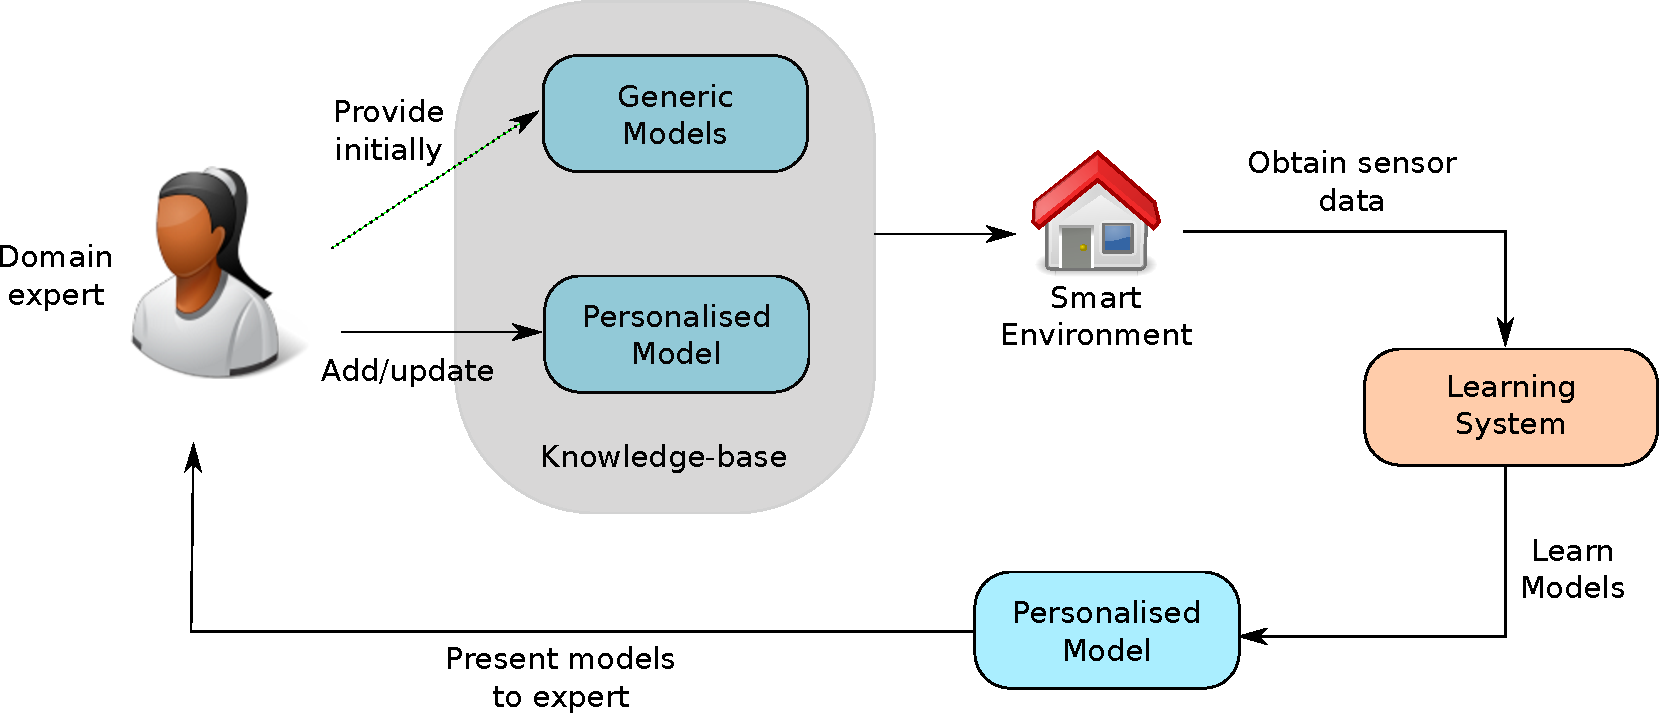
\includegraphics[width=\textwidth]{activity_modelling.pdf}
    \caption{The continuous activity model process to obtain dynamic and personalised models from generic expert provided models.}
    \label{fig-activity-modelling}
\end{figure}

In this dissertation, a continuous activity modelling process is presented, where domain experts provide initially generic activity models using knowledge engineering tools, to afterwards run data-driven learning algorithms on user generated data to learn personalised models. Such personalised models will be presented to the expert, who can add or update them in the knowledge-base. This loop is continuously repeated in time to achieve dynamic and personalised models based on initially provided generic models and user generated data. Figure \ref{fig-activity-modelling} shows a diagram with the described process.

The described activity modelling process uses generic knowledge-driven activity models provided by a domain expert, achieving thus generic and understandable activity models. To solve the problem of personalised models, user generated data is used in a learning process to produce knowledge-driven personalised models. This means that data-driven learning techniques are used to capture personal features of generic activities and obtain understandable personalised activity models. Such models, after expert validation, are added to the knowledge-base to use them subsequently in activity recognition systems. Repeating this process continuously, dynamic activity models are obtained, which evolve in time as users change - or not - their habits.

% One of the key elements of this process is the learning system, which has to learn new actions for already defined activities -> this is the target of the thesis; provide an example (MakeCoffee) with its image

When modelling activities, two major aspects are considered: the actions carried out to perform the activity and the descriptive features of the activity \cite{Chen2014}. Actions refer to object interactions. For example, to prepare a coffee a user might have coffee and a cup to drink the coffee. This sequence can be modelled as the action sequence of \textit{hasCoffee} and \textit{hasContainer}, which are obtained from the interactions with the respective objects monitored by sensors. Descriptive properties of an activity refer to the time when the activity has been performed, its duration, the concrete set of objects used and their order. Both aspects of an activity model, i.e. actions and descriptive properties, may vary from person to person. 

As far as learning personalised descriptive properties for knowledge-driven models regards, Chen et al. already combined data-driven and knowledge-driven approaches in \cite{Chen2014}. However, to the best of our knowledge, a similar work to learn specific actions for activity models has not been published yet. In fact, Chen et al. assume in their work that the actions in the \textit{seed} activity models provided by domain experts can be used for any user. This means that every user has to execute the same actions to perform a concrete activity.

In this dissertation, the problem of learning actions for given activities is analysed. It cannot be generally assumed that every user executes the same actions to perform a concrete activity. Imagine, for instance, that a user prepares a coffee and adds sugar to it. To make it simple, the activity model for this user could contain the actions \textit{hasCoffee}, \textit{hasContainer}, \textit{hasWater} and \textit{hasFlavour}. But there is another user who does not like any flavourant, so she prepares coffee by means of actions \textit{hasCoffee}, \textit{hasContainer} and  \textit{hasWater}. As it can be seen, both activity models are different as far as actions regard, but both of them are valid models for the activity of making a coffee. 

To develop a proper activity modelling process, learning actions is a key feature. It has been observed that generic activity models provided by a domain expert have the necessary actions to perform an activity, but not sufficient actions for personalised models. Those activity models can be used to further learn new actions for different users and thus generate new personalised activity models. Let us illustrate our hybrid activity modelling approach with an example. Figure \ref{fig-objective} shows an initial generic activity model for the MakeCoffee activity, which is composed by the actions \textit{hasCoffee} and \textit{hasContainer}. These are the necessary actions for every person to perform a MakeCoffee activity, which highlight the indispensable actions of making a coffee, i.e. the use of coffee and a container to place the coffee in. Nevertheless, some users might add some milk and sugar, others cream etc. The idea of our approach is to create high-level activity models with only these indispensable actions - generic models -, and then use the data generated by a specific user performing the activity to learn those new actions which also configure the personal way of making coffee. In the case of Figure \ref{fig-objective}, where the initial activity model will only include coffee and container, the system would learn that MakeCoffee is performed in two ways by the user: in the first one, the user adds milk (\textit{hasMilk}) and sugar (\textit{hasFlavour}), while in the second one only sugar is added (\textit{hasFlavour}). Hence two specialised and complete activity models of MakeCoffee can be learned. This way, experts, initially, only have to provide generic but incomplete activity models with necessary actions. Afterwards the learning system can analyse a user's behavioural data and learn the specialised and complete models to enrich the knowledge-base, thus improving initial activity models.

Running the proposed learning process periodically with new data generated by a concrete user, a dynamic activity modelling system is achieved. As a user evolves regarding the way she performs certain activities, the learning approach learns new versions of the initial activity models. Hence, activity models can be adapted to users' varying behaviours.

\begin{figure}[htbp]
\centering
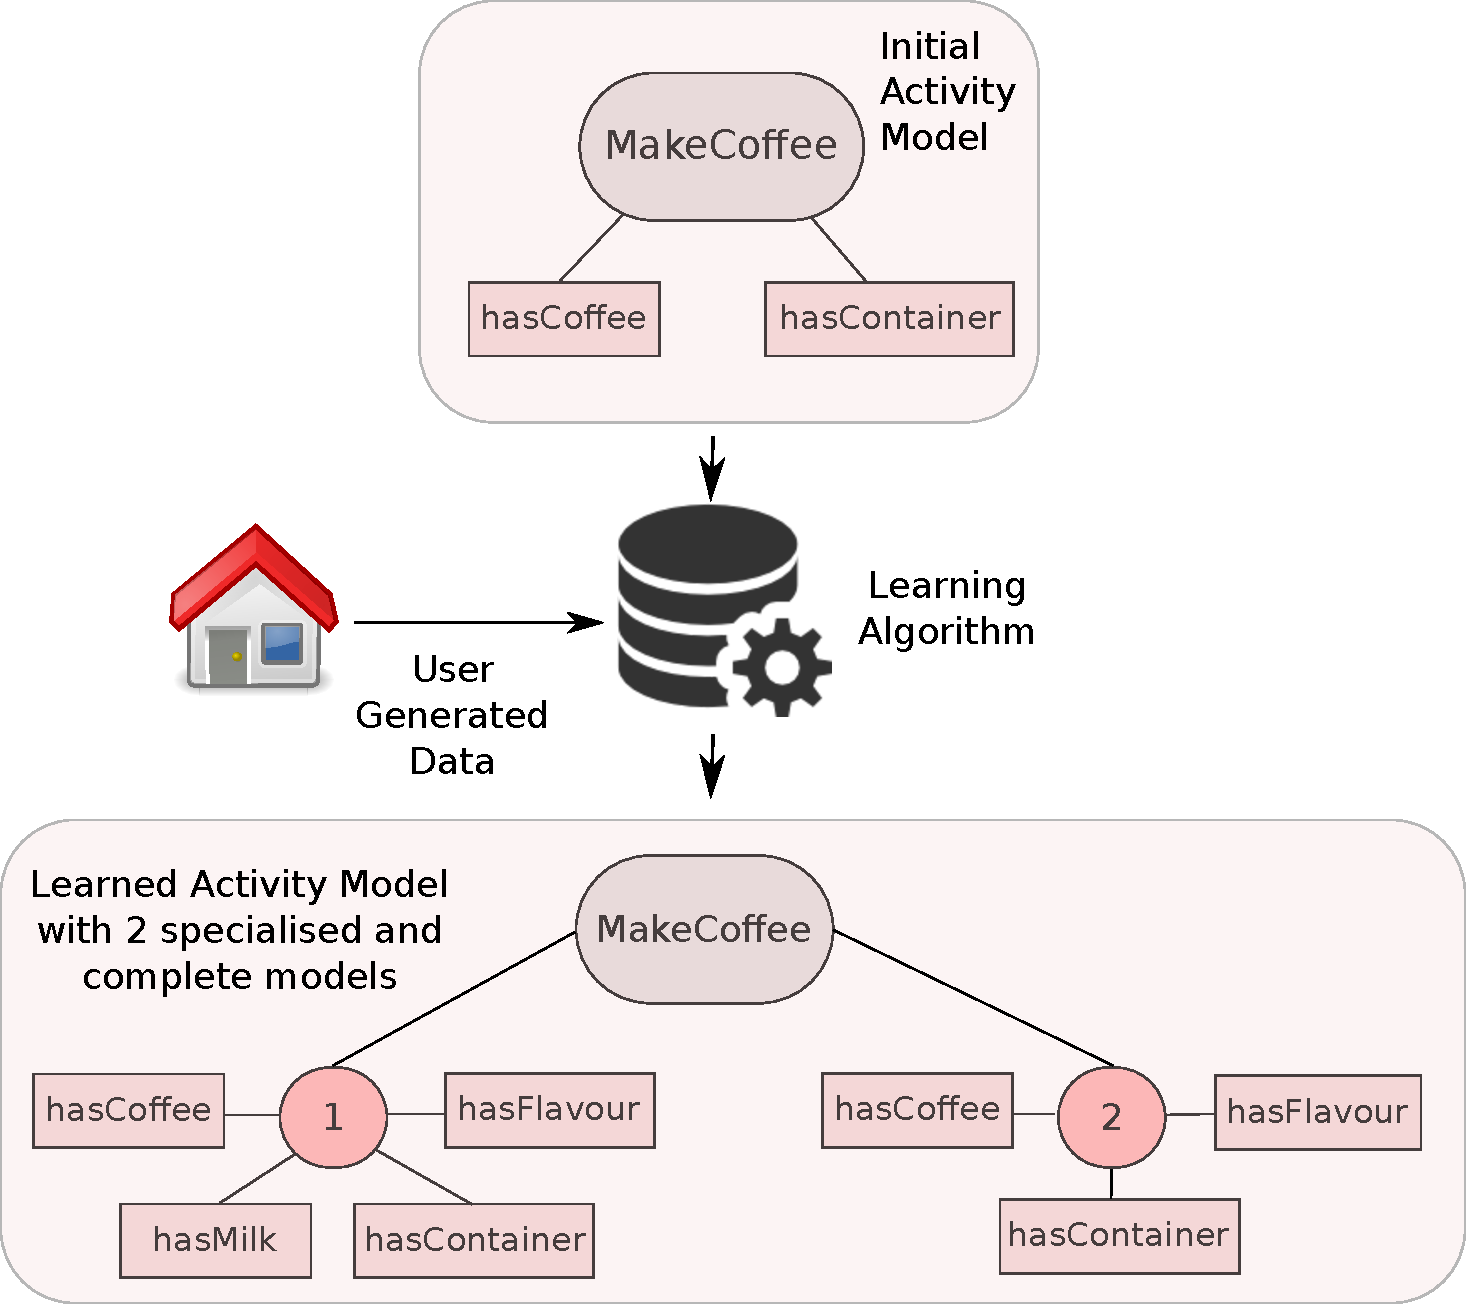
\includegraphics[width=9cm]{objective.pdf}
    \caption{Illustrative example of the objective of the dissertation: using the initial incomplete model for MakeCoffee and user generated data, the learning algorithm learns 2 specialised and complete models.}
    \label{fig-objective}
\end{figure}

Notice that the proposed modelling approach does not only learn new actions for initial activity models, but it also learns sub-activities of already defined activities. In the example depicted in Figure \ref{fig-objective}, the two specialised models are two sub-activities of the MakeCoffee activity, namely MakeBlackCoffee and MakeCoffeeWithMilk. This feature makes possible for the expert to define activities in a higher level of abstraction and let the system learn different sub-activities to generate specialised knowledge. 

As a summary, this dissertation is focused on making another step towards dynamic and personalised activity models for knowledge-driven activity recognition systems. A learning system to obtain complete and specialised activity models from generic but incomplete expert provided models has been developed. This step allows implementing activity modelling approaches that use expert knowledge to have generic activity models applicable to every user, and learn new actions for concrete users achieving personalised and dynamic activity models. 
\section{Motivation}
\label{sec:intro:motivation}

Why is this dissertation interesting? Justify it.


\section{Hypothesis, Objectives and Limitations}
\label{sec:intro:hypothesis}

%Write the hypothesis.

Based on the current state of activity modelling and recognition, the hypothesis of this dissertation is:

\vspace{0.5cm}

\noindent\fbox{
    \parbox{\textwidth}{
    \begin{hypo}
Using domain experts' previous knowledge as generic but incomplete activity models and data-driven learning techniques on user generated data, it is possible to learn accurately new actions to obtain personalised activity models for every user. 
\end{hypo}
}
}

\vspace{0.5cm}

To be able to validate this hypothesis the general goal of this dissertation is:

\vspace{0.5cm}

\noindent\fbox{
    \parbox{\textwidth}{
\begin{goal}
To design and implement a learning system that uses generic but incomplete activity models to analyse unlabelled sensor datasets generated by several users while performing some concrete activities and acquire personalised models which contain new actions.
\end{goal}
}
}

\vspace{0.5cm}


%Decompose hypothesis in smaller goals and objectives.

This general objective can be achieved by addressing the following more specific problems:

\begin{enumerate}
 \item To study the current state of the art on knowledge- and data-driven activity modelling and recognition.
 \item To choose a knowledge representation formalism and design proper structures to represent domain experts' knowledge.
 \item To design and implement a multiple step learning algorithm which uses previous knowledge and user generated data to obtain personalised activity models.
 \item To identify the most suitable evaluation methodology for the learning system.
 \item To validate the obtained results quantitatively, with the objective of capturing the 100\% of real activity models performed by a user. 
\end{enumerate}

The resulting learning system should also fulfil the following requirements:

\begin{enumerate}
 \item User independence: the learning system should be able to acquire personalised models for any user.
 \item Use the same generic activity models for every user: to show that incomplete activity models provided by experts are really generic, the same models have to be used for every user.
 \item Environment-independent: the knowledge representation formalism and the learning algorithm should be defined to cope with different environments. As such, representing new locations and objects of a different environment should be straightforward.
\end{enumerate}

%Describe constraints and limitations.

The work presented in this dissertation does not deal with the following conditions:

\begin{enumerate}
 \item Unknown activities: this dissertation does not propose any method to identify and learn unknown activities. Personalised models of already defined activities are learned, thus leaving the integration of other techniques to learn unknown activities for future work.
 \item Multiple users being monitored: it is assumed that only one user will be monitored in a particular experiment and dataset. Considering multi-user monitoring approaches is out of the scope of this research work.
 \item Concurrent and interwoven activities: users are not allowed to perform activities concurrently, i.e. once they start an activity, they have to finish it before starting another activity. Concurrent and interwoven activities pose challenges that will not be addressed in this dissertation.
 \item Online learning: the learning system will not be able to work online. Datasets will be processed offline using batch training systems.
\end{enumerate}




\section{Methodology}
\label{sec:intro:methodology}

A research strategy has been defined in order to achieve the statement and derived goals presented
in Section \ref{sec:intro:hypothesis}. The strategy is defined as follows:

\begin{enumerate}
    \item Update knowledge by reviewing the literature in the area of activity modelling and recognition, knowledge engineering, machine learning and data mining. This analysis has been reinforced by attending specialised scientific conferences.
    \item Critically evaluate existing activity modelling and recognition solutions, analysing their scope and limitations and identifying weak areas where contributions to the state of the art can be done.
    \item Design and develop the different modules of the activity model learner, incrementally adopting more complex and efficient solutions.
    \item Test developed modules through experiments and analyse results to enhance the performance of the system.
    \item Attend conferences and workshops to present partial results and validate them with the scientific community.
    \item Experimentation and evaluation of the prototype at each particular stage.
    \item Network with experts at conferences, project meetings and consortia (the author is an active member of the SONOPA project\footnote{http://www.sonopa.eu/} - SOcial Networks for Older adults to Promote an Active Life -). Contact for particular details by e-mail or by visiting other research groups (the author was a visiting researcher in De Montfort University for 6 weeks in 2014).
    \item Redesign the activity model learner system with feedback from all this network, as well as the literature.
    \item Select an appropriate evaluation methodology and evaluate consequently the activity model learner system.
    \item Dissemination of the results obtained during the research process.
\end{enumerate}

This methodology is illustrated in \myfig{fig-methodology}, as a cyclic process which starts with the review of the state of the art and finishes with the publications and the final prototype.

\begin{figure}[htbp]
\centering
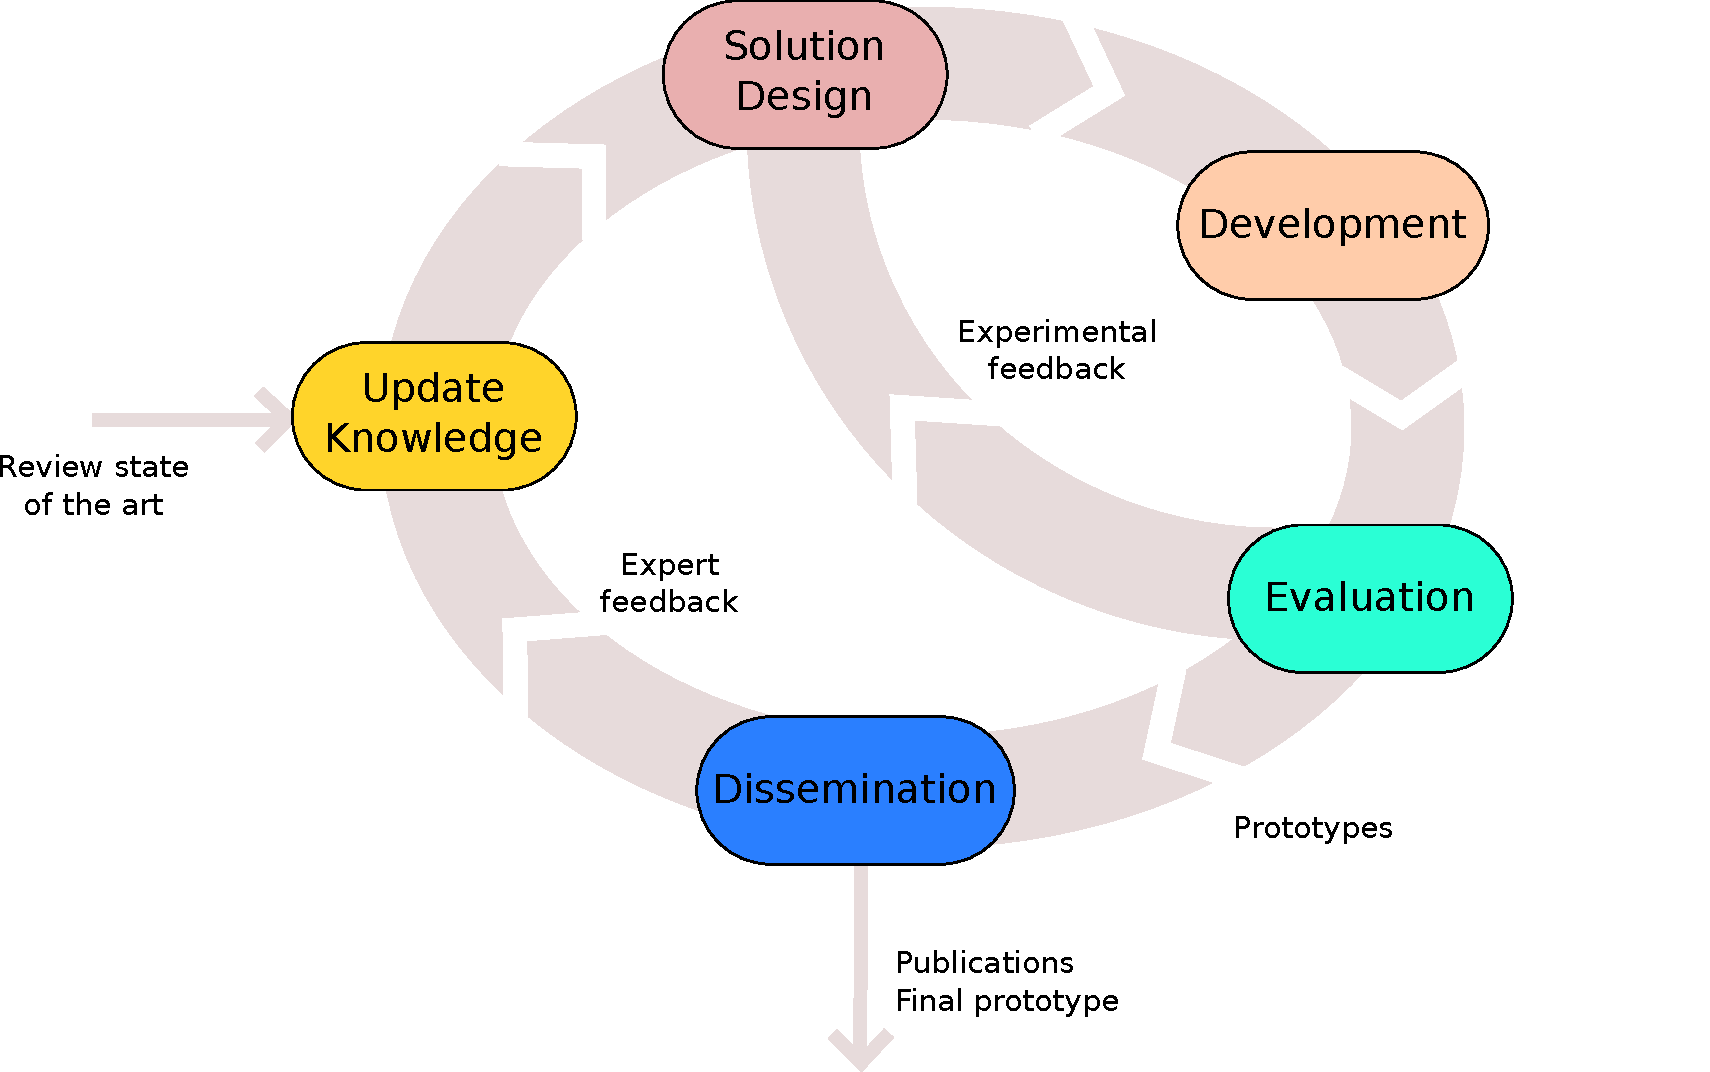
\includegraphics[width=\textwidth]{ball_methodology.pdf}
    \caption{Followed research methodology.}
    \label{fig-methodology}
\end{figure}



\section{Contributions}
\label{sec:intro:contributions}

%The following major and minor contributions can be found in this dissertation:
The following scientific contributions can be found in this dissertation:

\begin{itemize}
  \item A two-step activity clustering algorithm which uses generic but incomplete activity models and context knowledge to recognise action clusters that form an activity and aggregate new actions. The activity clustering algorithm idea is introduced in Chapter \ref{cha:archi} and it is explained thorough Chapter \ref{cha:clustering}.
  \item A learning algorithm that uses activity clusters to learn personalised activity models for every defined activity. This learning algorithm is first presented in Chapter \ref{cha:archi} and further developed in Chapter \ref{cha:learner}.
  \item A hybrid evaluation methodology for activity modelling and recognition, based on surveys to users and simulation tools. This evaluation methodology is fully described and applied in Chapter \ref{cha:evaluation}. The details of the methodology can be found in Section \ref{subsec:evaluation:hybrid}.
\end{itemize}

In order to deliver those scientific contributions, a technical contribution has also be posed in this dissertation:

\begin{itemize}
 \item A synthetic dataset generator tool: a special simulation tool for sensor dataset generation designed and developed to apply the hybrid evaluation methodology to the activity modelling approach. The software tool is described in Chapter \ref{cha:evaluation}, concretely in Section \ref{subsubsec:evaluation:synthetic}.
\end{itemize}



%: ----------------------- related work ------------------------


% this file is called up by thesis.tex
% content in this file will be fed into the main document

%: ----------------------- introduction file header -----------------------
\begin{savequote}[50mm]
If I have seen further it is by standing on the shoulders of giants.
\qauthor{Isaac Newton}
\end{savequote}

\chapter{Related Work}
\label{cha:soa}

% the code below specifies where the figures are stored
\ifpdf
    \graphicspath{{2_state_of_the_art/figures/PDF/}{2_state_of_the_art/figures/PNG/}{2_state_of_the_art/figures/}}
\else
    \graphicspath{{2_state_of_the_art/figures/EPS/}{2_state_of_the_art/figures/}}
\fi

%\letra{D}{escribe} how the state of the art has been structured in this chapter, referencing sections and commenting on their contents. Justify the topics covered by the chapter.

\letra{H}{uman} activity recognition is a broad research area which can be analysed from many different points of view. The objective of this chapter is to provide a high-level picture of the current status of the research topic, to then describe more in detail the concrete approaches that are related to the work presented in this dissertation. 

First of all, Section \ref{sec:soa:har} introduces the concept of \textit{Human Activity Recognition}, shows its main applications and provides a high-level taxonomy of activity recognition approaches. Section \ref{sec:soa:sensor} describes in detail the category in which this dissertation fits regarding the monitoring approach: \textit{Sensor-Based Activity Recognition}. Based on the specific sensors used for activity monitoring, Section \ref{sec:soa:monitoring} presents a more detailed taxonomy for the category of sensor-based activity recognition. On the other hand, the following sections analyse the main currents of activity modelling, which is the focus of this dissertation: Section \ref{sec:soa:datadriven} presents \textit{Data-Driven Approaches}, while Section \ref{sec:soa:knowledgedriven} describes in detail \textit{Knowledge-Driven Approaches}. A summary and comparison of both activity modelling currents is provided in Table \ref{tab:soa:comparison}. Some recent work has settled the basis to combine both currents, giving as result the \textit{Hybrid approaches}, as shown in Section \ref{sec:soa:hybrid}. This dissertation is another step in order to achieve hybrid approaches that can combine effectively the best features of knowledge- and data-driven approaches. The chapter finalises with Section \ref{sec:soa:summary}, where a concise summary is provided alongside with some conclusions.
\section{Human Activity Recognition}
\label{sec:soa:har}

%Talk about human activity recognition as a research topic. Explain in what application it has been used, how and for what and different sensor approaches used. Make clear that this dissertation will be based on sensor-based activity recognition.

Human activity recognition has become a key research topic in diverse areas, including pervasive and mobile computing \cite{Weiser1991} \cite{Choudhury2008}, surveillance-based security \cite{Poppe2010}, \cite{Akdemir2008}, \cite{Weinland2011}, context-aware computing \cite{Laerhoven2001}, \cite{Wren2006}, ambient assisted living \cite{Philipose2004}, \cite{Cook2009}, \cite{Kasteren2008}, \cite{Chen2012a} and social robotics \cite{Fong2003a}. The recent increase in interest in activity recognition can be attributed to the intensive thrusts from the latest technology development and application demands. The progress in sensor technologies has been substantial over the past decade, especially low-power, low-cost, high-capacity and miniaturised sensors, wired and wireless communication networks \cite{Pantelopoulos2010}, \cite{Alemdar2010}, \cite{Ding2011}. In parallel, data processing techniques have also shown important advances, based on higher computational capabilities of devices and the development of novel algorithms. The progress and maturity of these supporting technologies have pushed the research focuses of the aforementioned areas to shift from low-level data collection and transmission towards high-level information integration, context processing and activity recognition and inference. 

At the same time, activity recognition has been demanded by a growing number of solutions for real-world problems and applications. For example, surveillance and security try to make use of activity recognition technologies to address the threats of terrorists \cite{Akdemir2008}. Ambient assisted living aims to exploit activity monitoring, recognition and assistance to support independent living and ageing in place. Other emerging applications, such as intelligent meeting rooms \cite{Mikic2000} and smart hospitals \cite{Sanchez2008}, are also dependent on activity recognition in order to provide multimodal interactions, proactive service provision, and context aware personalised activity assistance. 

As a result of the technology push and application pull, activity recognition has built its own space in the academic world. As such, research related to activity recognition has become regular topics in mainstream international conferences in related areas such as the AAAI Conference on Artificial Intelligence\footnote{http://www.aaai.org/}, Computer Vision and Pattern Recognition\footnote{http://www.cvpr201x.org/}, International Joint Conference on Artificial Intelligence\footnote{http://ijcai.org/}, International Joint Conference on Pervasive and Ubiquitous Computing\footnote{http://ubicomp.org/}, International Conference on Pervasive Computing and Communications\footnote{http://www.percom.org/} and International Joint Conferences on Ambient Intelligence\footnote{http://www.ami-conferences.org/}. In order to try to channel the research towards future applications, a substantial number of projects and initiatives have been undertaken. Good examples are \textit{The Ambient Assisted Living Joint Programme}\footnote{www.aal-europe.eu}, \textit{The House of the Future}\footnote{http://architecture.mit.edu/house\_n}, \textit{The Gator-Tech Smart House}\footnote{http://www.icta.ufl.edu/gt.htm} or \textit{The iDorm project}\footnote{http://cswww.essex.ac.uk/iieg/idorm.htm}.  %In addition, a growing number of workshops have been dedicated to activity recognition research from different research angles and communities. For example, in 2011 alone eight workshops were specifically devoted to activity recognition research, including IWFAR [24], HAU3D [25], SAGAware [26], PAIR [27], GAPRec [28] and others [29][30][31]. The interest and enthusiasm for this topic is still increasing.

Apart from potential applications, activity recognition has gained research interest because it is a multidisciplinary and complex process. Activity recognition can be roughly characterised by four basic tasks. These tasks include:
\begin{enumerate}
 \item Selection and deployment of appropriate sensors to objects and environments in order to monitor and capture a user’s behaviour along with the state change of the environment.
 \item To collect, store and process perceived information through data analysis techniques and/or knowledge representation formalisms at appropriate levels of abstraction.
 \item To create computational activity models in a way that allows software systems/agents to conduct reasoning and manipulation.
 \item To select or develop reasoning algorithms to infer activities from sensor data.
\end{enumerate}

Each individual task can be tackled by a great variety of methods, technologies and tools. It is often the case that the selection of a method used for one task is dependent on the method of another task. As such, activity recognition has been classified in the following ways according to \cite{Chen2012}. The first classification criterion focuses on the sensors used for activity monitoring, while the second one pays attention to activity modelling techniques:

\begin{enumerate}
 \item \textbf{Vision-based vs. sensor-based activity recognition:} In terms of the type of sensor that is used for activity monitoring, activity recognition can be generally classified into two categories. The first is referred to as vision-based activity recognition, which is based on the use of visual sensing facilities such as video cameras to monitor an actor’s behaviour and environmental changes. The generated sensor data are video sequences or digitized visual data. The approaches in this category exploit computer vision techniques, including feature extraction, structural modelling, person and object recognition, movement segmentation, action extraction and movement tracking to analyse visual observations for pattern recognition. The second category is referred to as sensor-based activity recognition, which is based on the use of emerging sensor network technologies for activity monitoring (Section \ref{sec:soa:sensor}). The generated sensor data from sensor-based monitoring are mainly time series of state changes and/or various parameter values that are usually processed through data fusion, probabilistic or statistical analysis methods and formal knowledge technologies for activity recognition. Sensor-based activity monitoring can be further classified into two categories: (i) wearable sensor-based activity monitoring, where sensors are attached to an actor under observation, and (ii) dense sensing-based activity monitoring, where sensors are attached to objects that constitute the activity environment. Wearable sensors, including modern smartphones, often use inertial measurement units and RFID tags to gather an actor’s behavioural information. This approach is effective for recognising physical movements such as physical exercises. In contrast, dense sensing infers activities by monitoring human-object interactions through the usage of multiple multi-modal miniaturised sensors.

 \item \textbf{Data-driven vs. knowledge-driven activity recognition:} The information obtained through activity monitoring has to be structured and processed to recognise activities. For that purpose, activity models play a critical role. In particular, the mechanisms activities are recognised are closely related to the nature and representation of activity models. Generally speaking, activity models can be built using one of two methods. The first is to learn activity models from pre-existent large-scale datasets of users’ behaviours using data mining and machine learning techniques. This method involves the creation of probabilistic or statistical activity models, followed by training and learning processes. As this method is driven by data, and the ensued activity inference is based on probabilistic or statistical classification, it is often referred to as data-driven or bottom-up approaches (in the rest of this dissertation, data-driven will be used to refer to this category). The advantages of the data-driven approaches are the capabilities of handling uncertainty and temporal information \cite{Brand1997}. However, this method requires large datasets for training and learning, and suffers from the data scarcity or the “cold start” problem. It is also difficult to apply learnt activity models from one person to another. As such this method suffers from the problems of scalability and reusability. Data-driven approaches are described in detail in Section \ref{sec:soa:datadriven}. The other method for building activity models is to exploit rich prior knowledge in the domain of interest to construct activity models directly using knowledge engineering and management technologies. This usually involves knowledge acquisition, formal modelling and representation. Activity models generated in this method are normally used for activity recognition or prediction through formal logical reasoning, e.g., deduction, induction or abduction. As such, this method is referred to as knowledge-driven or top-down approach (knowledge-driven will be used from now on). Knowledge-driven approaches have the advantages of being semantically clear, logically elegant and easy to get started. But they are weak in handling uncertainty and temporal information and the models could be viewed as static and incomplete. For a complete review of knowledge-driven approaches, see Section \ref{sec:soa:knowledgedriven}. With the purpose of combining the advantages of those two methods, hybrid approaches have recently emerged (Section \ref{sec:soa:hybrid}). 
\end{enumerate}

The situation generated by both classification criteria is represented in Figure \ref{fig-classification}, providing a high-level view of activity recognition systems' taxonomy.

\begin{figure}[htbp]
\centering
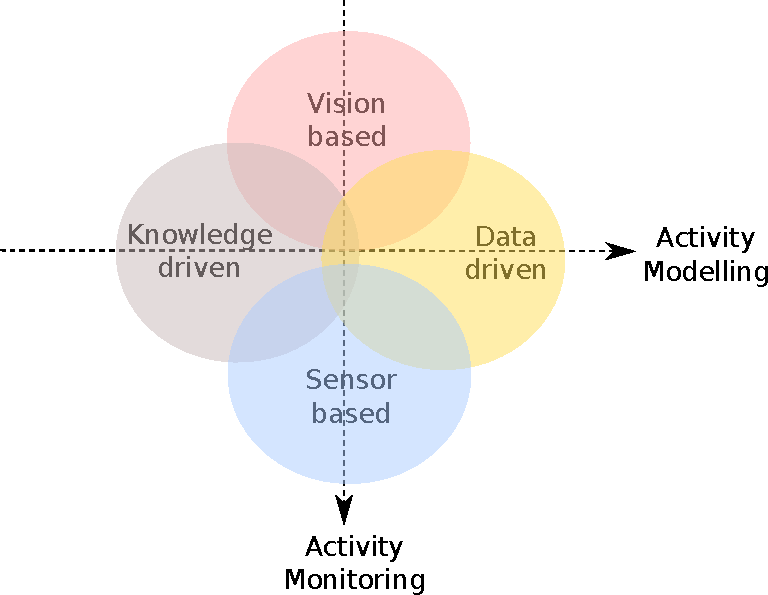
\includegraphics[width=11cm]{activity_taxonomy-m.pdf}
    \caption{A high-level taxonomy of activity recognition systems, spanned by two axis: monitoring and modelling approach.}
    \label{fig-classification}
\end{figure}
 
Vision-based activity recognition has been a research focus for a long period of time due to its important role in areas such as surveillance, robot learning and security. However, as this dissertation is based on sensor-based approaches, an exhaustive review of vision-based systems is not provided. Detailed up to date reviews can be found in \cite{Poppe2010}, \cite{Moeslund2006}, \cite{Yilmaz2006}, \cite{Weinland2011} and \cite{Turaga2008}. Even though all those surveys cover different topics, together they have provided an extensive overview on the vision-based approach. It is concluded from those contributions that while visual monitoring is intuitive and information-rich, vision-based activity recognition suffers from issues relating to privacy and ethics \cite{Yilmaz2006} as cameras are generally perceived as recording devices.

Compared to the number of surveys in vision-based activity recognition, and considering the wealth of literature in sensor-based activity recognition, there is a lack of extensive review on the state of the art of sensor-based activity recognition. This may be because the approach only recently became feasible when the sensing technologies matured to be realistically deployable in terms of the underpinning communication infrastructure, costs and sizes. An exception to this rule is the survey published by Chen et al. \cite{Chen2012}, which can be considered as the reference work for any sensor-based activity recognition approach. 

\section{Sensor-Based Activity Recognition}
\label{sec:soa:sensor}

For the upcoming discussions about activity monitoring, modelling and recognition, it is useful to distinguish human behaviours at different levels of granularity. For physical behaviours, the terms “action” and “activity” are commonly used in activity recognition communities. In some cases they are used interchangeably and in other cases they are used to denote behaviours of different complexity and duration. In the latter cases the term “action” is usually referred to as simple ambulatory behaviour executed by a single person and typically lasting for short durations of time. Examples of actions include bending, retrieving a cup from a cupboard, opening a door, putting a teabag into a cup and so forth. On the other hand, the term “activities” here refers to complex behaviours consisting of a sequence of actions and/or interleaving or overlapping actions. They could be performed by a single human or several humans who are required to interact with each other in a constrained manner. They are typically characterized by much longer temporal durations, such as making tea or two persons making meals. For the rest of this dissertation, the second case will be adopted. As such, ``actions'' will be considered short-time simple executions, while ``activities'' will be described by a sequence of actions.

The first approaches that implemented the idea of using sensors for activity monitoring and recognition appeared in the late 90s. The \textit{Neural Network House} \cite{Mozer1998}, in the context of home automation, can be considered a pioneer in this area, alongside with a number of location-based applications aiming to adapt systems to users’ whereabouts \cite{Leonhardt1998}, \cite{Golding1999}, \cite{Ward1997}. The approach was soon found to be more useful and suitable in the area of ubiquitous and mobile computing – an emerging area in the late 90s, due to its easy deployment. As such, extensive research has been undertaken to investigate the use of sensors in various application scenarios of ubiquitous and mobile computing, leading to considerable work on context-awareness \cite{Schmidt1999}, \cite{Randell2000}, \cite{Gellersen2002}, smart appliances \cite{Schmidt2001}, \cite{Laerhoven2001} and activity recognition \cite{Laerhoven2001a}, \cite{Foerster2000}, \cite{Lee2002}. Those initial research works usually made use of wearable sensors, either dedicated sensors attached to human bodies or portable devices like mobile phones, with application to ubiquitous computing scenarios such as providing context-aware mobile devices. Activities being monitored in these researches are mainly physical activities like motion, walking and running. These early works lay a solid foundation for wearable computing and still inspire and influence today’s research.

In the early 2000s, a new sensor-based approach that uses sensors attached to objects to monitor human activities appeared. This approach, which was later dubbed as the “dense sensing” approach, performs activity recognition through the inference of user-object interactions \cite{Bao2004}, \cite{Patterson2003}. The approach is particularly suitable for dealing with activities that involve a number of objects within an environment, or instrumental Activities of Daily Living (ADL) \cite{Chan2008}, \cite{Nugent2009}. Research on this approach has been heavily driven by the intensive research interests and huge research effort on smart home based assisted living, such as the EU’s Ambient Assisted Living program. In particular, sensor-based activity recognition can better address sensitive issues in assisted living such as privacy, ethics and obtrusiveness than conventional vision-based approaches. This combination of application needs and technological advantages has stimulated considerable research activities in a global scale, which gave rise to a large number of research projects, where a plethora of impressive works on sensor-based activity recognition have been developed \cite{Kern2003}, \cite{Mantyjarvi2001}, \cite{Philipose2004}, \cite{Patterson2005}, \cite{Buettner2009}, \cite{Wren2006}, \cite{Gu2009}, \cite{Patterson2003}, \cite{Liao2007}.

While substantial research has been undertaken, and significant progress has been made, the two main approaches, wearable sensors based and dense sensing based activity recognition are currently still focuses of study. The former is mainly driven by the ever-popular pervasive and mobile computing while the latter is predominantly driven by smart environment applications such as ambient assisted living. Interests in various novel applications are still increasing and application domains are rapidly expanding.

\section{Sensor and Activity Monitoring}
\label{sec:soa:monitoring}

Thanks to the rapid development in electronics, a wide range of sensors, including contact sensors, RFID, accelerometers, audio and motion detectors, to name but a few, are available for activity monitoring. These sensors are different in types, purposes, output signals, underpinning theoretical principles and technical infrastructure. However, they can be classified into two main categories in terms of the way they are deployed in activity monitoring applications. These are wearable sensors and dense sensors, and are described in detail in the following sections.

\subsection{Wearable sensor-based activity monitoring}

Wearable sensors generally refer to sensors that are positioned directly or indirectly on human body. These kinds of sensors can be worn by humans, so they are named wearable sensors. They generate signals when the user performs actions and activities. As a result, they can monitor features that are descriptive of the person’s physiological state or movement. Wearable sensors can be embedded into clothes, eyeglasses, belts, shoes, wristwatches, mobile devices or positioned directly on the body. They can be used to collect information such as body position and movement, pulse, and skin temperature. Researchers have found that different types of sensor information are effective for classifying different types of activities. As wearable sensors are not directly related to this dissertation, some references are shown for further reading, classified by the sensors used:

\begin{enumerate}
 \item Inertial measurement units: those sensors are composed by accelerometers and gyroscopes and are probably the most frequently used wearable sensor for activity monitoring. Inertial measurement units provide information about acceleration and speed of the units while moving. In consequence, they are appropriate to monitor human movements and actions and activities related to body motion, such as physical exercise. Some  examples of the usage of inertial measurement units are provided in \cite{Bao2004}, \cite{Lukowicz2004}, \cite{Lee2002} and \cite{Mantyjarvi2001}.
 \item GPS sensors: specially used for monitoring outdoor location-based activities, such as in \cite{Patterson2003}, \cite{Ashbrook2003} and \cite{Liao2007a}.
 \item Biosensors: to monitor activities through vital signs, e.g. \cite{Sung2004}, \cite{Harms2008} and \cite{Finni2007}.
\end{enumerate}

Wearable sensor-based activity monitoring suffers from limitations. Most wearable sensors need to run continuously and be operated hands-free. This may have difficulties in real world application scenarios. Practical issues include the acceptability or willingness to use wearable sensors and the viability and ability to wear them. Technical issues include the size, ease of use, battery life and effectiveness of the approach in real-world scenarios. A way to overcome such problems is to make use of existing gadgets that have already been carried in a daily basis like smartphones as intelligent sensors for activity monitoring, recognition and assistance. This practice has been in place for a while \cite{Gellersen2002}, \cite{Schmidt2001} and is expected to gain large-scale uptake given the latest development and affordability of such palm-held electronic devices. Recently, a new and promising class of wearable sensors have appeared in the market, namely the Google Glasses\footnote{https://www.google.com/glass/start/} (see Figure \ref{fig-google-glass}). Those special glasses include a camera, a small eye-screen, headphones and a computing unit. It is expected that the irruption of such glasses will bring to market more similar options. The potential of these kinds of devices for activity monitoring and recognition is still to be explored. 

Obviously wearable sensors are not suitable for monitoring activities that involve complex physical motions and/or multiple interactions with the environment. In some cases, sensor observations from wearable sensors alone are not sufficient to differentiate activities involving simple physical movements (e.g., making tea and making coffee). As a result, dense sensing based activity monitoring has emerged, which is described below.

\begin{figure}[htbp]
\centering
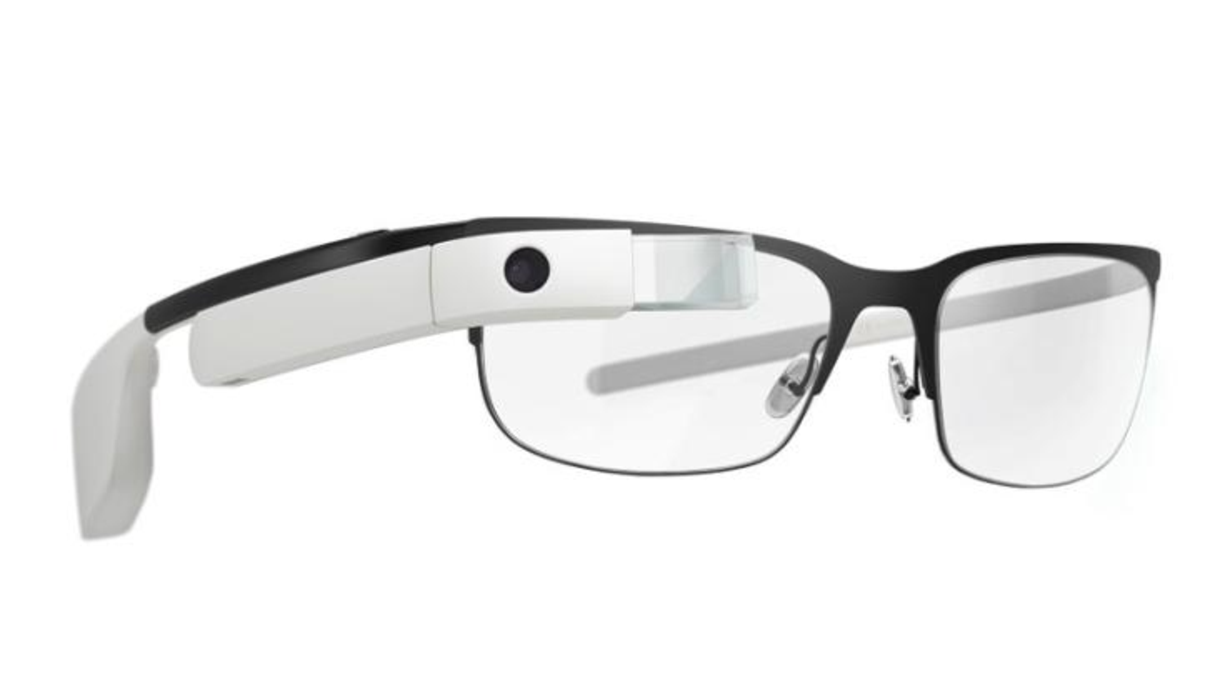
\includegraphics[width=9cm]{google-glass.pdf}
    \caption{The Google Glass wearable, with its processing unit, camera, headphones and screen.}
    \label{fig-google-glass}
\end{figure}

\subsection{Dense sensing-based activity monitoring}

Dense sensing-based activity monitoring is based on attaching sensors to objects that a user manipulates while performing activities. Hence activity monitoring is carried out by detecting user-object interactions. The approach is based on real-world observations that activities are characterised by the objects that are manipulated during their performance. A simple indication of an object being used can often provide powerful clues about the activity being undertaken. As such it is assumed that activities can be recognised from sensor data that monitors human interactions with objects in the environment. By dense sensing, the way and scale with which sensors are used is characterised. Using dense sensing a large number of sensors, normally low-cost low-power and miniaturised, are deployed in a range of objects or locations within an environment for the purpose of monitoring movement and behaviour. Following the dense sensing paradigm, sensors are moved from human bodies to human-populated environments.

The dense sensing paradigm has been widely used for creating ambient intelligent applications such as smart homes, because sensors are embedded within environments. The pre-eminence of dense sensing in ambient assisted living (AAL), via the smart home paradigm, can be seen in \cite{Chan2008}, \cite{Nugent2009} or \cite{Helal2005}. Sensors in a smart home can monitor an inhabitant’s movements and environmental events so that activities can be inferred based on the sensor observations, thus providing just-in-time context-aware assistance. For instance, a switch sensor in the bed can strongly suggest sleeping or relaxing, and pressure mat sensors can be used for tracking the movement and position of people within the environment.

Since the introduction of the idea in early 2000s \cite{Bao2004}, \cite{Patterson2003}, extensive research has been undertaken to investigate the applicability of the approach in terms of sensor types, modalities and applications. For example, Tapia et al. \cite{Tapia2004} use environmental state-change sensors to collect information about interaction with objects and recognise activities that are of interest to medical professionals such as toileting, bathing, and grooming. Wilson et al. \cite{Wilson2005} use four kinds of anonymous and binary sensors, motion detectors, break-beam sensors, pressure mats, and contact switches for simultaneous tracking and activity recognition. Wren et al. \cite{Wren2006} employ networks of passive infrared motion sensors to detect presence and movement of heat sources. With this captured data they can recognise low-level activities such as walking, loitering, and turning, as well as mid-level activities such as visiting and meeting. Srivastava et al. \cite{Srivastava2001} exploit wireless sensor network to develop smart learning environment for young children. Hollosi et al. \cite{Hollosi2010} use voice detection techniques to perform acoustic event classification for monitoring in Smart Homes. Simple object sensors are adopted in \cite{Aipperspach2006}.

Given the abundance of different types and modalities of sensors, sensors have been used in different ways and combinations for dense sensing activity monitoring in many application scenarios. It is impossible to claim that one sensor deployment for a specific application scenario is superior to the other. The suitability and performance is usually down to the nature of the type of activities being assessed and the characteristics of the concrete applications. 

Generally speaking, wearable sensor-based activity monitoring receives more attention in mobile computing while dense sensing is more suitable for intelligent environment enabled applications. It is worth pointing out that wearable sensors and dense sensing are not mutually exclusive. In some applications they have to work together. For example, RFID (Radio Frequency Identification) based activity monitoring requires that objects are instrumented with tags and users wear an RFID reader affixed to a glove or a bracelet. Philipose and Fishkin \cite{Philipose2004}, \cite{Fishkin2005} developed two devices, iGlove and iBracelet, working as wearable RFID readers that detect when users interact with unobtrusively tagged objects. Patterson et al. \cite{Patterson2005} performed fine-grained activity recognition (i.e., not just recognising that a person is cooking but determining what they are cooking) by aggregating abstract object usage. Hodges et al. \cite{Hodges2007} proposed to identify individuals from their behaviour based on their interaction with the objects they use in performing daily activities. Buettner et al. \cite{Buettner2009} recognise indoor daily activities by using an RFID sensor network. In most cases wearable sensors and dense sensing are complementary and can be used in combination in order to yield optimal recognition results. For example, Gu et al. \cite{Gu2009} combine wearable sensors and object sensors for collecting multimodal sensor information. Through a pattern-based method, they recognise sequential, interleaved and concurrent activities.

Dense sensing activity monitoring has also some drawbacks. One of the most obvious ones is the need to install a lot of sensors in human populated environments, which may involve considerable infrastructure changes (install pressure mats or movement sensors), or the problem of adding sensors to any new object introduced in the environment (attach contact sensors to glasses bought in the supermarket). The practical feasibility of the approach is probably linked to introducing sensors in the production steps of objects and building phases of the environments. Another drawback is the simple information provided by the sensors, which cannot be enough if very detailed activities have to be recognised. A contact sensor may indicate an interaction between a human and an object, but it cannot provide any information about how the object is being used by the human. 
\section{Data-Driven Approaches}
\label{sec:soa:datadriven}

In terms of the techniques and methods used for activity modelling and recognition, abstracting from specific activity monitoring systems, data-driven activity modelling is one of the most successful approaches. Data-driven activity modelling can be generally classified into two main categories: generative and discriminative. The generative approach attempts to build a complete description of the input or data space, usually with a probabilistic model such as a Bayesian Network. In contrast, the discriminative approach only models the mapping from inputs (data) to outputs (activity labels). Discriminative approaches include many heuristic (rule-based) approaches, neural networks, conditional random fields and linear or non-linear discriminative learning (e.g. support vector machines). Results using each of those methods are covered in the following.

\subsection{Generative modelling}

The simplest possible generative approach is the Na\"ive Bayes classifier, which has been used with promising results for activity recognition \cite{Bao2004} \cite{Brdiczka2007} \cite{Cook2009} \cite{Tapia2004} \cite{Kasteren2007} \cite{Maurer2006a}. Na\"ive Bayes classifiers model all observations (e.g. sensor readings) as arising from a common causal source: the activity, as given by a discrete label. The dependence of observations on activity labels is modelled as a probabilistic function that can be used to identify the most likely activity given a set of observations. Despite the fact that these classifiers assume conditional independence of the features, the classifiers yield good accuracy when large amounts of sample data are provided. Nevertheless, Na\"ive Bayes classifiers do not explicitly model any temporal information, usually considered important in activity recognition.

The Hidden Markov Model (HMM) is probably the most popular generative approach that includes temporal information. A HMM is a probabilistic model with a particular structure that makes it easy to learn from data, to interpret the data once a model is learned, and is both easy and efficient to implement. It consists of a set of hidden (latent) states coupled in a stochastic Markov chain, such that the distribution over states at some time depends only on the values of states at a finite number of preceding times. The hidden states then probabilistically generate observations through a stochastic process. HMMs made their impact initially through use in the speech recognition literature, where latent states correspond to phoneme labels, and observations are features extracted from audio data. HMMs have more recently been adopted as a model of choice in computer vision for modelling sequential (video) data (see \cite{Gavrila1999} \cite{Moeslund2006} for surveys and \cite{Galata1999} \cite{Starner1995} for early examples). HMMs use a Markov chain over a discrete set of states. A closely relative of the HMM uses continuous states, a model usually referred to as a linear dynamical system (LDS). State estimation in LDSs is better known as a Kalman filter. LDSs have been used with inputs from a variety of sensors for physiological condition monitoring \cite{Quinn2009} in which a method is also introduced to deal with unmodelled variations in data, one of the major shortcomings of the generative approach.

HMMs form the basis of statistical temporal models. They are, in fact, a special case of the more general Dynamic Bayesian Networks (DBNs), which are Bayesian networks in which a discrete time index is explicitly represented. Inference and learning in DBNs is simply an application of network propagation in Bayesian networks. DBNs usually make a Markovian assumption, but explicitly represent conditional independence in the variables, allowing for more efficient and accurate inference and learning. A well known early use of DBNs for activity monitoring was in the \textit{Lumi\'ere} project, where a Microsoft Windows user’s need for assistance was modelled based on their activities on the screen \cite{Horvitz1998}.

A simple DBN extension of HMMs is the coupled HMM for recognition of simultaneous human actions (e.g. pedestrian motions \cite{Brand1997}). Coupled Hidden Markov Models (CHMMs) have two Markovian chains, each modelling a different stream of data, with a coupling between them to model their inter-dependence. Oliver et al. \cite{Oliver2004} learn a multi-layer model of office activity to choose actions for a computational agent. The model uses multimodal inputs, making only very slight use of computer vision. The Assisted Cognition project \cite{Kautz2002} has made use of DBNs, in particular for Opportunity Knocks \cite{Liao2007a}, a system designed to provide directional guidance to a user navigating through a city. This system uses a three level hierarchical Markov model represented as a DBN to infer a user’s activities from GPS sensor readings. Movement patterns, based on the GPS localization signals, are translated into a probabilistic model using unsupervised learning. From the model and the user’s current location, future destinations and the associated mode of transportation can be predicted. Based on the prediction, the system has the ability to prompt the user if an error in route is detected.

Wilson and Atkeson use DBNs to simultaneously track persons and model their activities from a variety of simple sensors (motion detectors, pressure sensors, switches, etc.) \cite{Wilson2005}. DBNs were also used in the iSTRETCH system, a haptic robotic device to assist a person with stroke rehabilitation \cite{Kan2011}. The DBN models the person’s current behaviours, their current abilities, and some aspects of their emotional state (e.g. their responsiveness, learning rate and fatigue level). The person’s behaviours correspond to how long they take for each exercise, what type of control they exhibit and whether they compensate. These behaviours are inferred from sensors on the device and in the person’s chair.

Even though they are simple and popular, HMMs and DBNs have some limitations. A HMM is incapable of capturing long-range or transitive dependencies of the observations due to its very strict independence assumptions (on the observations). Furthermore, without significant training, a HMM may not be able to recognise all of the possible observation sequences that can be consistent with a particular activity.

\subsection{Discriminative modelling}

A drawback of the generative approach is that enough data must be available to learn the complete probabilistic representations that are required. In this section, an alternative approach for modelling is discussed, in which the focus is on solving the classification problem, rather than on the representation problem. The complete data description of a generative model induces a classification boundary, which can be seen by considering every possible observation and applying the classification rule using inference. The boundary is thus implicit in a generative model, but a lot of work is necessary to describe all the data to obtain it. A discriminative approach, on the other hand, considers this boundary to be the primary objective.

Perhaps the simplest discriminative approach is Nearest Neighbour (NN), in which a novel sequence of observations is compared to a set of template sequences in a training set, and the most closely matching sequences in the training set vote for their activity labels. This simple approach can often provide very good results. Bao and Intille investigated this method along with numerous other base-level classifiers for the recognition of activities from accelerometer data \cite{Bao2004}. They found that the simple NN approach is outperformed by decision trees, a related method, where the training data is partitioned into subsets according to activity labels and a set of rules based on features of the training data. The rules can then be used to identify the partition (and hence the activity label) corresponding to a new data sample. Maurer et al. \cite{Maurer2006a}, employed decision trees to learn logical descriptions of activities from complex sensor readings from a wearable device (the eWatch). The decision tree approach offers the advantage of generating rules that are understandable by the user, but it is often brittle when high precision numeric data is collected. Stikic and Schiele use a clustering method in which activities are considered as a “bag of features” to learn template models of activities from data with only sparse labels \cite{Stikic2009}. 

For the classification problem, the points closest to the boundary are the ones that give more information about the boundary itself. Points lying far apart the boundary should not be taken into account then. There are several discriminative approaches that effectively take advantage of this fact. The challenge is therefore to find these “hard” data points (the ones closest to the boundary). These data points will be known as the “support vectors”, and actually define the boundary. A support vector machine (SVM) is a machine learning technique to find these support vectors automatically. A recent example of an SVM in use for activity modelling is presented by Brdiczka et al. \cite{Brdiczka2009} where a model of situations is learned automatically from data by first learning roles of various entities using SVMs and labelled training data, then using unsupervised clustering to build ’situations’ or relations between entities, which are then labelled and further refined by end users. The key idea in this work is to use a cognitive model (situation model) based on cognitive theory motivated by models of human perception of behaviour in an environment. The CareMedia project \cite{Chen2005} also uses an SVM to locate and recognise social interactions in a care facility from multiple sensors, including video and audio. The fusion of video and audio allowed 90\% recall and 20\% precision in identifying interactions including shaking hands, touching, pushing and kicking. The CareMedia project’s goals are to monitor and report behaviour assessments in a care home to caregivers and medical professionals.

Ravi et al. also found that SVMs performed consistently well, but also investigated meta-level classifiers that combined the results of multiple base-level classifiers \cite{Ravi2005}. Features extracted from worn accelerometers are extracted and classified using five different base-level classifiers (decision tables, decision trees, k-NN, SVM and Na\"ive Bayes). The meta-level classifiers are generated through a variety of techniques such as boosting, bagging, voting, cascading and stacking. For recognising a set of eight activities including standing, walking, running, going up/down stairs, vacuuming and teeth brushing, they found that a simple voting scheme performed the best for three easier experimental settings, whereas boosted SVM performed best for the most difficult setting (test/training separation across users and days)

In practice, many activities may have non-deterministic natures, where some steps of the activities may be performed in any order, and so are concurrent or interwoven. A conditional random field (CRF) is a more flexible alternative to the HMM that addresses such practical requirements. It is a discriminative and generative probabilistic model that represents the dependence of a hidden variable $y$ on an observed variable $x$ \cite{Sutton2007}. Both HMMs and CRFs are used to find a sequence of hidden states based on observation sequences. Nevertheless, instead of finding a joint probability distribution $p(x,y)$ as the HMM does, a CRF attempts to find only the conditional probability $p(y|x)$. A CRF allows for arbitrary, non-independent relationships among the observation sequences, hence the added flexibility. Another major difference is the relaxation of the independence assumptions, in which the hidden state probabilities may depend on the past and even future observations. A CRF is modelled as an undirected acyclic graph, flexibly capturing any relation between an observation variable and a hidden state. CRFs are applied to the problem of activity recognition in \cite{Vail2007} where they are compared to HMMs, but only in a simple simulated domain. Liao et al. use hierarchical CRFs for modeling activities based on GPS data \cite{Liao2007}. Hu and Yang use skip-chain CRFs, an extension in which multiple chains interact in a manner reminiscent of the CHMM, to model concurrent and interleaving goals \cite{Hu2008}, a challenging problem for activity recognition. Mahdaviani and Choudhury show how semi-supervised CRFs can be used to learn activity models from wearable sensor data \cite{Mahdaviani2008}.

\subsection{Other approaches}

There are many approaches in the literature which cannot be clearly classified into discriminative or generative categories, but rather use a combination of both. The Independent Lifestyle Assistant (ILSA) is an example, as it uses a combination of heuristic rules and statistical models of sequential patterns of sensor firings and time intervals to help a person with planning and scheduling \cite{Guralnik2002}. PEAT (the Planning and Execution Assistant and Trainer) is a cognitive assistant that runs on a mobile device, and helps compensate for executive functional impairment. PEAT uses reactive planning to adjust a user’s schedule based on their current activities. Activity recognition in PEAT is based on what the user is doing, and on data from sensors on the mobile device. These are fed into a HMM, the outputs of which are combined with the reactive planning engine \cite{Modayil2008}.

Other work has investigated how activities can be modelled with a combination of discriminative and generative approaches \cite{Lester2005}, how common sense models of everyday activities can be built automatically using data mining techniques \cite{Pentney2008} \cite{Pentney2007}, and how human activities can be analysed through the recognition of object use, rather than the recognition of human behaviour \cite{Wu2007}. This latter work uses DBNs to model various activities around the home, and a variety of radio frequency identification (RFID) tags to bootstrap the learning process. Some authors have attempted to compare discriminative and generative models \cite{Bao2004} \cite{Ravi2005}, generally finding the discriminative models yield lower error rates on unseen data, but are less interpretable. Gu et al. use the notion of emerging patterns to look for frequent sensor sequences that can be associated with each activity as an aid for recognition \cite{Gu2009}. Omar et al. present a comparative study of a variety of classification methods for analysing multi-modal sensor data from a smart walker \cite{Omar2010}.

% Rashidi and Cook's work could go here
One of the biggest problems of data-driven approaches, regardless their category, is the need of large-scale labelled data bases. This problem arises because activity recognition is posed as a supervised learning problem. However, due to the required effort and time for annotating activity data bases, supervised methods do not scale up well in practice. Annotating activity data imposes a burden on annotators and users and often introduces a source of error in the process. Rashidi and Cook show how to overcome the problem of depending on labelled activity data bases in \cite{Rashidi2011}, improving the approach in \cite{Rashidi2013}. They use a non-labelled data base, where they extract activity clusters using unsupervised learning techniques. More concretely, they develop a new activity discovery method named COM, which stands for Continuous, varied Order, Multi Threshold. COM not only discovers discontinuous patterns and their variations, but is able to better handle real life data by dealing with different frequencies/sensor problem. All patterns discovered by COM are then used as inputs for a hierarchical agglomerative clustering algorithm. The clustering algorithm aims at grouping those sensor patterns which are similar in terms of their structure. An activity structure is defined as the start time, duration and region or location. Those clusters are finally used to train a boosted HMM, which is shown to be able to recognise discovered activities. 

Rashidi and Cook bring a new paradigm to data-driven activity recognition in their works, showing the real possibility of using an unsupervised model and avoid data base annotation problems. However, their approach still suffers some other traditional problems of data-driven approaches. Firstly, even though they do not use labelled data bases, they do not overcome the ``cold start'' problem, since they have to collect data in order to discover activities and train HMMs. Besides, as other data-driven approaches, they have many difficulties when generalising what they have discovered and learned from previous users, since every user has his/her own ways of performing activities. The price to pay for avoiding labelled data bases is that the approach cannot set activity granularity and that discovered activities do not have any semantic meaning. The first problem refers to the impossibility of deciding at design phase what kind of activities will be recognised. For example, if a user usually washes dishes after preparing meal, COM will discover this sequence as a typical activity. However, the discovered activity is actually a sequence of two lower-grain activities. The second problem refers to the fact that discovered activities are only sequences of sensors with their location and time information, but without any semantic meaning. A human expert is needed afterwards to interpret discovered activities and label them with semantic tags. Notice that this \textit{a posteriori} labelling step may be difficult since activity granularity is not set. 

% Finish with advantages and drawbacks of those approaches

\subsection{Summary of data-driven approaches}

Data-driven approaches have been extensively used for activity recognition. Their advantages and disadvantages are very well known by the scientific community (a summary and comparison to knowledge-driven approaches can be found in Table \ref{tab:soa:comparison}):

\subsubsection*{Advantages}
\begin{itemize}
 \item Uncertainty modelling: as probabilistic and statistical activity modelling is used, data-driven approaches are very good modelling sensor uncertainty. As sensors do not provide certain information and are exposed to failures, modelling uncertainty is a very important feature for real-world deployments.
 \item Temporal information modelling: modelling approaches such as DBNs, HMMs and similar implicitly model temporal information of activities, such as time lapses between two sensor readings, activity duration or activity start time. Time information can be learned from data in a natural way.
 \item Introduce heuristics: discriminative approaches make possible introducing heuristics about activity models. Heuristics can be used to insert basic knowledge about activities and avoid making activity models totally dependent on data.
 \item Dynamic activity models: as learning is a continuous process, activity models evolve as the user changes its habits. As such, activity models are dynamic.
 \item Personal activity models: learning activity models directly over user data, makes activity models personalised. This means that activity models capture the particular way of performing an activity by a user.
\end{itemize}

\subsubsection*{Disadvantages}
\begin{itemize}
 \item ``Cold start'' problem: data is needed to model activities. The dependency with data arises the ``cold start'' problem, since data-driven techniques cannot work immediately after deployment. A data collecting and activity model training process is required for every user.
 \item Lack of reusability: as activity models are directly learned from concrete user data, they cannot generally be used for other users. The main problem is that data-driven approaches cannot build generic activity models, only personal activity models.
 \item Dataset annotation problems: if annotated datasets are needed (supervised learning approaches), scalability becomes a real problem, since the effort required for annotation is huge and annotation methods are prone to errors. If annotated datasets are not used (unsupervised approach), activity granularity and activity semantics is lost. 
\end{itemize}


\section{Knowledge-Driven Approaches}
\label{sec:soa:knowledgedriven}

It has been observed that for most activities the list of objects required for a particular activity is limited and functionally similar. Knowledge-driven activity modelling is motivated by those observations. The idea is that even if the activity can be performed in different ways the number and type of involved objects do not vary significantly. For example, it is common sense that the activity “make coffee” consists of a sequence of actions involving a coffee pot, hot water, a cup, coffee, sugar and milk; the activity “brush teeth” contains actions involving a toothbrush, toothpaste, water tap, cup and towel. On the other hand, as humans have different life styles, habits or abilities, they may perform various activities in different ways. For instance, one may like strong white coffee and another may prefer a special brand of coffee. Even for the same type of activity (e.g., making white coffee), different individuals may use different items (e.g., skimmed milk or whole milk) and in different orders (e.g., adding milk first and then sugar, or vice versa). Such domain-dependent activity-specific prior knowledge provides valuable insights into how activities can be constructed in general and how they can be performed by individuals in specific situations.

Similarly, knowledge-driven activity recognition is founded upon the observations that most activities, in particular, routine activities of daily living and working, take place in a relatively specific circumstance of time, location and space. The space is usually populated with events and entities pertaining to the activities, forming a specific environment for specific purposes. For example, brushing teeth is normally undertaken twice a day in a bathroom in the morning and before going to bed and involves the use of toothpaste and a toothbrush; meals are made in a kitchen with a cooker roughly three times a day. The implicit relationships between activities, related temporal and spatial context and the entities involved (objects and people) provide a diversity of hints and heuristics for inferring activities.

Knowledge-driven activity modelling and recognition intends to make use of rich domain knowledge and heuristics for activity modelling and pattern recognition. The rationale is to use various methods, in particular, knowledge engineering methodologies and techniques, to acquire domain knowledge. The captured knowledge can then be encoded in various reusable knowledge structures, including activity models for holding heuristics and prior knowledge in performing activities, and context models for holding relationships between activities, objects and temporal and spatial contexts. Comparing to data-driven activity modelling that learns models from large-scale datasets and recognises activities through data intensive processing methods, knowledge-driven activity modelling avoids a number of problems, including the requirement for large amounts of observation data, the inflexibility that arises when each activity model needs to be computationally learned, and the lack of reusability that results when one person’s activity model is different from another’s. 

Knowledge structures can be modelled and represented in different forms, such as schemas, rules or networks. This will decide the way and the extent to which knowledge is used for further processing such as activity recognition, prediction and assistance. In terms of the manner in which domain knowledge is captured, represented and used, knowledge-driven approaches to activity modelling and recognition can be roughly classified into three main categories as presented in the following sections.

\subsection{Mining-based approach}

The objective of a mining-based approach is to create activity models by mining existing activity knowledge from publicly available sources. More specifically, given a set of activities, the approach seeks to discover from the text corpuses a set of objects used for each activity and extract object usage information to derive their associated usage probabilities. The approach essentially views an activity model as a probabilistic translation between activity names (e.g., “make coffee”) and the names of involved objects (e.g., “mug”, “milk”). As the correlations between activities and their objects are common-sense prior knowledge (e.g., most of us know how to carry out daily activities), such domain knowledge can be obtained from various sources such as how-tos (e.g., those at \textit{ehow.com} or \textit{wikihow.com}), recipes (e.g., from \textit{epicurious.com}), training manuals, experimental protocols, and facility/device user manuals.

A mining-based approach consists of a sequence of distinct tasks. Firstly it needs to identify activities of concern and relevant sources that describe these activities. Secondly, it uses various methods, predominantly information retrieval and analysis techniques, to retrieve activity definitions from specific sources and extract phrases that describe the objects used during the performance of the activity. Then algorithms, predominantly probabilistic and statistic analysis methods such as co-occurrences and association are used to estimate the object-usage probabilities. Finally, the mined object and usage information is used to create activity models such as a HMM that can be used further for activity recognition. 

Mining-based activity modelling was initially investigated by researchers from Intel Research \cite{Wu2007} \cite{Wyatt2005}. Perkowitz et al. \cite{Perkowitz2004} proposed the idea of mining the Web for large-scale activity modelling. They used the QTag tagger to tag each word in a sentence with its part of speech (POS) and a customized regular expression extractor to extract objects used in an activity. They then used the Google Conditional Probabilities (GCP) APIs to determine automatically the probability values of object usage. The mined object and their usage information are then used to construct DBN models through Sequential Monte Carlo (SMC) approximation. They mined the website \textit{ehow.com} for roughly 2300 directions on performing domestic tasks (from “boiling water in the microwave” to “change your air filter”), and the website \textit{ffts.com} and \textit{epicurious.com} for a further 400 and 18,600 recipes respectively, generating a total 21,300 activity models. Using the DBN activity models they have performed activity recognition for a combination of real user data and synthetic data. While initial evaluation results were positive, the drawback was that there are no mechanisms to guarantee the mined models capturing completely the sequence probabilities and the idiosyncrasy of certain activities. The inability to capture such intrinsic characteristics may limit the model's accuracy in real deployments.

Wyatt et al. \cite{Wyatt2005} followed Perkowitz’s approach by mining the Web to create DBN activity models. However, this group extended the work in three aspects, aiming to address the idiosyncrasies and to improve model accuracy. To cover the wide variety of activity definition sources, they mined the Web in a more discriminative way in a wider scope. They did this by building a specialised genre classifier trained and tested with a large number of labelled Web pages. To enhance model applicability, they used the mined models as base activity models and then exploited the Viterbi Algorithm and Maximum Likelihood to learn customized activity parameters from unsegmented, unlabelled sensor data. In a bid to improve activity recognition accuracy they also presented a bootstrap method that produced labelled segmentations automatically. Then they used the Kullback-Leibler (KL) divergence to compute activity similarity.

A difficulty in connecting mined activities with tagged objects \cite{Perkowitz2004} \cite{Wyatt2005} is that the activity models may refer to objects synonymously. For example, both a “mug” and “cup” can be used for making tea; both a “skillet” and “frying pan” may be used for making pasta. This leads to a situation that one activity may have different models with each having the same activity name but different object terms. To address this, Tapia et al. \cite{Tapia2006} proposed to extract collections of synonymous words for the functionally-similar objects automatically from WordNet, an online lexical reference system for the English language. The set of terms for similar objects is structured and represented in a hierarchical form known as the object ontology. With the similarity measure provided by the ontology, an activity model will not only cover a fixed number of object terms but also any other object terms that are in the same class in the ontology. 

Another shortcoming of early work in the area \cite{Perkowitz2004} \cite{Wyatt2005} is that the segmentation is carried out in sequential order based on the duration of an activity. As the duration of performing a specific activity may vary substantially from one to another, this may give rise to applicability issues. In addition, in sequential segmentation one error in one segment may affect the segmentations of the subsequent traces. To tackle this, Palmes et al. \cite{Palmes2010} proposed an alternate method for activity segmentation and recognition. Instead of relying on the order of object use, they exploited the discriminative trait of the usage frequency of objects in different activities. They constructed activity models by mining the Web and extracting relevant objects based on their weights. The weights are then utilised to recognise and segment an activity trace containing a sequence of objects used in a number of consecutive and non-interleaving activities. To do this, they proposed an activity recognition algorithm, KeyExtract, which uses the list of discriminatory key objects from all activities to identify the activities present in a trace. They further proposed two heuristic segmentation algorithms, MaxGap and MaxGain, to detect the boundary between each pair of activities identified by KeyExtract. Boundary detection is based on the calculation, aggregation, and comparison of the relative weights of all objects sandwiched in any two key objects representing adjacent activities in a trace. Though the mining based approach has a number of challenges relating to information retrieval, relation identification and the disambiguation of term meaning, nevertheless, it provides a feasible alternative to model large amount of activities. Initial research has demonstrated the approach is promising. 

Mining-based approaches are similar to data-driven approaches in that they all adopt probabilistic or statistical activity modelling and recognition. But they are different from each other in the way that the parameters of the activity models are decided. The mining-based approaches make use of publicly available data sources avoiding the “cold start” problem. Nevertheless they are weak in dealing with idiosyncrasies of activities. On the other hand, data-driven approaches have the strength of generating personalised activity models, but they suffer from issues such as “cold start” and model reusability for different users.

\subsection{Logic-based approaches}

A logic-based approach views an activity as a knowledge model that can be formally specified using various logical formalisms. From this perspective, activity modelling is equivalent to knowledge modelling and representation. As such, systematic knowledge engineering methodologies and techniques are used for domain knowledge acquisition and formal construction of activity structures. Knowledge representation formalisms or languages are used to represent these knowledge models and concrete knowledge instances, thus enabling inference and reasoning. In this way, activity recognition and other advanced application features such as prediction and explanation can be mapped to knowledge-based inference such as deduction, induction and abduction. 

Logic-based approaches are composed of a number of distinct tasks. Even though each task can be undertaken in different ways the role of each task is specific and unique. Normally the first step is to carry out knowledge acquisition, which involves eliciting knowledge from various knowledge sources such as domain experts and activity manuals. The second step is to use various knowledge modelling techniques and tools to build reusable activity structures. This will be followed by a domain formalization process in which all entities, events and temporal and spatial states pertaining to activities, along with axioms and rules, are formally specified and represented using representation formalism. This process usually generates the domain theory. The following step will be the development of a reasoning engine in terms of knowledge representation formalisms to support inference. In addition, a number of supportive system components will be developed, which are responsible for aggregating and transforming sensor data into logical terms and formula. With all functional components in place, activity recognition proceeds by passing the logical representation of sensor data onto the reasoning engine. The engine performs logical reasoning, e.g., deduction, abduction or induction, against the domain theory. The reasoning will extract a minimal set of covering models of interpretation from the activity models based on a set of observed actions, which could semantically explain the observations.

There exist a number of logical modelling methods and reasoning algorithms in terms of logical theories and representation formalisms. One thread of work is to map activity recognition to the plan recognition problem in the well studied artificial intelligence field \cite{Carberry2001}. The problem of plan recognition can be stated in simple terms as: given a sequence of actions performed by an actor, how to infer the goal pursued by the actor and also to organise the action sequence in terms of a plan structure. Kautz et al. \cite{Kautz1991} adopted first-order axioms to build a library of hierarchical plans. They proposed a set of hypotheses such as exhaustiveness, disjointedness and minimum cardinality to extract a minimal covering model of interpretation from the hierarchy, based on a set of observed actions. Wobke \cite{Wobcke2002} extends Kautz’s work using situation theory to address the different probabilities of inferred plans by defining a partial order relation between plans in terms of levels of plausibility. Bouchard et al. \cite{Bouchard2006} borrow the idea of plan recognition and apply it to activity recognition. They use action Description Logic (DL) to formalize actions and entities and variable states in a smart home to create a domain theory. They model a plan as a sequence of actions and represent it as a lattice structure, which, together with the domain theory, provides an interpretation model for activity recognition. As such, given a sequence of action observations, activity recognition amounts to reasoning against the interpretation model to classify the actions through a lattice structure. It was claimed that the proposed DL models can organize the result of the recognition process into a structured interpretation model in the form of lattice, rather than a simple disjunction of possible plans without any classification. This minimises the uncertainty related to the observed actor’s activity by bounding the plausible plans set.

Another thread of work is to adopt the Event Calculus (EC) \cite{Shanahan1997} formalism, a highly developed logical theory of actions, for activity recognition and assistance. The EC formalizes a domain using fluents, events and predicates. Fluents are any properties of the domain that can change over time. Events are the fundamental instrument of change. All changes to a domain are the result of named events. Predicates define relations between events and fluents that specify what happens when and which fluents hold at what times. Predicates also describe the initial situation and the effects of events. Chen et al. \cite{Chen2008} proposed an EC-based framework in which sensor activations are modelled as events, and object states as properties. In addition, they developed a set of high- level logical constructors to model compound activities, i.e. the activities consisting of a number of sequential and/or parallel events. In the framework, an activity trace is simply a sequence of events that happen at different time points. Activity recognition is mapped to deductive reasoning tasks, e.g., temporal projection or explanation, and activity assistance or hazard prevention is mapped to abductive reasoning tasks. The major strength of this work is its capability to address temporal reasoning and the use of compound events to handle uncertainty and flexibility of activity modelling. 

Logic-based approaches are totally different from data-driven approaches in the way activities are modelled and the mechanisms activities are recognised. They do not require pre-existing large-scale datasets, and activity modelling and recognition is semantically clear and elegant in computational reasoning. It is easy to incorporate domain knowledge and heuristics for activity models and data fusion. The weakness of logical approaches is their inability or inherent infeasibility to represent fuzziness and uncertainty even though there are recent works trying to integrate fuzzy logics into the logical approaches. Another drawback is that logical activity models are viewed as one-size-fits-all, inflexible for adaptation to different users’ activity habits.

\subsection{Ontology-based approaches}
\label{subsec:soa:ontology}

Using ontologies for activity recognition is a recent endeavour and has gained growing interest. In the vision-based activity recognition community, researchers have realised that symbolic activity definitions based on manual specification of a set of rules suffer from limitations in their applicability, because the definitions are only deployable to the scenarios for which they have been designed. There is a need for a commonly agreed explicit representation of activity definitions or an ontology. Such ontological activity models are independent of algorithmic choices, thus facilitating portability, interoperability and reuse and sharing of both underlying technologies and systems. Chen et al. \cite{Chen2004} propose activity ontologies for analysing social interaction in nursing homes, Hakeem et al. \cite{Hakeem2004} for the classification of meeting videos, and Georis et al. \cite{Georis2004} for activities in a bank monitoring setting. To consolidate these efforts and to build a common knowledge base of domain ontologies, a collaborative effort has been made to define ontologies for six major domains of video surveillance. This has led to a video event ontology \cite{Nevatia2004} and the corresponding representation language \cite{Francois2005}. For instance, Akdemir \cite{Akdemir2008} used the video event ontologies for activity recognition in both bank and car park monitoring scenarios. In principle these studies use ontologies to provide common terms as building primitives for activity definitions. Activity recognition is performed using individually preferred algorithms, such as rule-based systems \cite{Hakeem2004} and finite-state machines \cite{Akdemir2008}. 

In the dense sensing-based activity recognition community, ontologies have been utilised to construct reliable activity models. Such models are able to match different object names with a term in an ontology which is related to a particular activity. For example, a Mug sensor event could be substituted by a Cup event in the activity model MakeTea as Mug and Cup can both be used for the MakeTea activity. This is particularly useful to address model incompleteness and multiple representations of terms. Tapia et al. \cite{Tapia2006} generated a large object ontology based on functional similarity between objects from WordNet, which can complete mined activity models from the Web with similar objects. Yamada et al. \cite{Yamada2007} use ontologies to represent objects in an activity space. By exploiting semantic relationships between things, the reported approach can automatically detect possible activities even given a variety of object characteristics including multiple representation and variability. Similar to vision-based activity recognition, these studies mainly use ontologies to provide activity descriptors for activity definitions. Activity recognition can then be performed based on probabilistic and/or statistical reasoning \cite{Tapia2006} \cite{Yamada2007}.

Ontology-based modelling and representation has been applied to general ambient assisted living. Latfi et al. \cite{Latfi2007} propose an ontological architecture of a telehealth-based smart home aiming at high-level intelligent applications for elderly persons suffering from loss of cognitive autonomy. Klein et al. \cite{Klein2007} developed an ontology-centred design approach to create a reliable and scalable ambient middleware. Chen et al. \cite{Chen2009} pioneered the notion of semantic smart homes in an attempt to leverage the full potential of semantic technologies in the entire lifecycle of assistive living i.e. from data modelling, content generation, activity representation, processing techniques and technologies to assist with the provision and deployment. While these endeavours, together with existing work in both vision- and dense sensing-based activity recognition, provide solid technical underpinnings for ontological data, object, sensor modelling and representation, there is a gap between semantic descriptions of events/objects related to activities and semantic reasoning for activity recognition. Most works use ontologies either as mapping mechanisms for multiple terms of an object \cite{Tapia2006} or the categorization of terms \cite{Yamada2007} or a common conceptual template for data integration, interoperability and reuse \cite{Latfi2007} \cite{Klein2007} \cite{Chen2009}. Activity ontologies which provide an explicit conceptualization of activities and their interrelationships have only recently emerged and have been used for activity recognition. Chen et al. \cite{Chen2009b} \cite{Chen2012a} proposed and developed an ontology-based approach to activity recognition. They constructed context and activity ontologies for explicit domain modelling. Sensor activations over a period of time are mapped to individual contextual information and then fused to build a context at any specific time point. They made use of subsumption reasoning to classify the constructed context based on the activity ontologies, thus inferring the ongoing activity. Ye et al. \cite{Ye2011} developed an upper activity ontology that facilitates the capture of domain knowledge to link the meaning implicit in elementary information to higher-level information that is of interest to applications. Riboni et al. \cite{Riboni2011b} investigated the use of activity ontologies, in particular, the new feature of rule representation and rule-based reasoning from OWL2, to model, represent and reason complex activities.

Compared with data-driven and mining-based approaches, ontology-based approaches offer several compelling features: firstly, ontological ADL models can capture and encode rich domain knowledge and heuristics in a machine understandable and processable way. This enables knowledge based intelligent processing at a higher degree of automation. Secondly, DL- based descriptive reasoning along a time line can support incremental progressive activity recognition and assistance as an ADL unfolds. The two levels of abstraction in activity modelling, concepts and instances, also allow coarse-grained and fine-grained activity assistance. Thirdly, as the ADL profile of an inhabitant is essentially a set of instances of ADL concepts, it provides an easy and flexible way to capture a user’s activity preferences and styles, thus facilitating personalised ADL assistance. Finally, the unified modelling, representation and reasoning for ADL modelling, recognition and assistance makes it natural and straightforward to support the integration and interoperability between contextual information and ADL recognition. This will support systematic coordinated system development by making use of seamless integration and synergy of a wide range of data and technologies. 

Compared with logic-based approaches, ontology-based approaches have the same mechanisms for activity modelling and recognition. However, ontology-based approaches are supported by a solid technological infrastructure that has been developed in the semantic Web and ontology-based knowledge engineering communities. Technologies, tools and APIs are available to help carry out each task in the ontology-based approach, e.g., ontology editors for context and activity modelling, web ontology languages for activity representation, semantic repository technologies for large-scale semantic data management and various reasoners for activity inference. This gives ontology-based approaches huge advantage in large-scale adoption, application development and system prototyping.

% Finish with advantages and drawbacks of these approaches
\subsection{Summary of knowledge-driven approaches}
The advantages and drawbacks of knowledge-driven approaches are summarised in the following listing. A summary and comparison with data-driven approaches can be found in Table \ref{tab:soa:comparison}.

\subsubsection*{Advantages}
\begin{itemize}
 \item No ``cold start'' problem: knowledge-driven approaches model activities using generic knowledge rather than data, so activity models are built before deployment and the system does not need any training/learning process before beginning to work.
 \item Interoperability and reusability: specially true for ontology-based approaches, but also for all the other approaches, as activity models are modelled using knowledge engineering techniques and built models are generic and not specific to a concrete user. 
 \item Clear semantics: activity models are semantically clear and can be understood by human beings. This allows interpreting how the system works and developing easier auxiliary systems that work on top of the activity recognition system, such as notification systems, recommender systems, etc. 
\end{itemize}

\subsubsection*{Disadvantages}
\begin{itemize}
 \item Weak in handling uncertainty: inference and reasoning are usually based on certain facts, rather than uncertain sensor information. There are some approaches that work using fuzzy logics and/or probabilistic reasoning, but they are not fully integrated with modelling techniques yet \cite{Helaoui2013} \cite{Almeida2012}.
 \item Weak in handling temporal information: inference and reasoning mechanisms used for activity recognition do not usually consider temporal aspects of activities. In order to tackle this limitation, there are already some approaches that, for example, integrate ontological and temporal knowledge modelling formalisms for activity modelling \cite{Okeyo2012}. 
 \item Static activity models: knowledge-based activity models are static, since once they are defined, they cannot automatically evolve. This means that if a user changes its way of performing activities, initially defined activity models will still be used for activity recognition.
\end{itemize}


% Insert comparative table here
\newcommand{\specialcell}[2][c]{%
  \begin{tabular}[#1]{@{}c@{}}#2\end{tabular}}

%\begin{table}[htbp]%\tiny
\begin{sidewaystable}[htbp]\scriptsize
    \begin{center}    
        \begin{tabular}{|c|c|c|c|c|c|c|}
            \hline            
            \multicolumn{1}{|c|}{} & \multicolumn{4}{c|}{\textbf{Knowledge-Driven Approaches}} & \multicolumn{2}{c|}{\textbf{Data-Driven Approaches}} \\
            \cline{2-7}
            \multicolumn{1}{|c|}{} & Mining-based & Logic-based & \multicolumn{2}{c|}{Ontology-based} & Generative & Discriminative \\             
            \hline
            \textbf{Model Type}   & \specialcell{HMM, DBN,\\SVM, CRF, NN} & \specialcell{Plans, lattices,\\event trees} & \specialcell{HMM, DBN,\\SVM, CRF, NN} & \specialcell{Sensor and\\Activity ontologies} & \specialcell{Na\"ive Bayes, HMM,\\LDS, DBN} & \specialcell{NN, SVM, CRF,\\Decision tree}  \\
            \hline
	    \specialcell{\textbf{Modelling}\\\textbf{Mechanism}} & \specialcell{Information\\retrieval and\\analysis} & \specialcell{Formal knowledge\\modelling} & \specialcell{(un)supervised\\learning from\\datasets} & \specialcell{Ontological\\engineering} & \specialcell{(un)supervised\\learning from\\datasets} & \specialcell{(un)supervised\\learning from\\datasets}\\
	    \hline
	    \specialcell{\textbf{Activity}\\\textbf{Recognition}\\\textbf{Method}} & \specialcell{Generative or\\discriminative\\methods} & \specialcell{Logical inference\\(deduction, induction)} & \specialcell{Generative or\\discriminative\\methods} & \specialcell{Semantic reasoning\\(subsumption, consistency)} & \specialcell{Probabilistic\\classification} & \specialcell{Similarity or rule\\based reasoning}\\
	    \hline
	    \textbf{Advantage} & \specialcell{No ``cold start''\\problem,\\Using multiple\\data sources} & \specialcell{No ``cold start''\\problem, clear\\semantics on modelling\\\& inference} & \specialcell{Shared terms,\\interoperability\\and reusability} & \specialcell{No ``cold start'' problem,\\multiple models, clear\\semantics on modelling \&\\inference, interoperability\\\& reusability}  & \specialcell{Modelling\\uncertainty,\\temporal\\information} & \specialcell{Modelling\\uncertainty,\\temporal\\information,\\heuristics} \\
	    \hline
	    \textbf{Disadvantage} & \specialcell{The same\\problem as\\DDA} & \specialcell{Weak in handling\\uncertainty and\\scalability}  & \specialcell{The same\\problem as\\DDA} & \specialcell{Weak in handling\\uncertainty and time} & \specialcell{``Cold start''\\problem, lack\\of reusability \&\\scalability} & \specialcell{``Cold start''\\problem, lack\\of reusability \&\\scalability} \\
            \hline
        \end{tabular}
        \caption{The summary and comparison of activity recognition approaches.}
        \label{tab:soa:comparison}
    \end{center}
\end{sidewaystable}
\section{Hybrid Approaches}
\label{sec:soa:hybrid}

Describe here the approach Chen approach to learn non-modelled activities and descriptive properties for modelled activities. Any other reference for hybrid approaches?
\section{Summary and Conclusions}
\label{sec:soa:summary}

%Put a table like the one we can find in Chen's survey paper, showing the strengths and weaknesses of each approach. Highlight which are the topics that are not covered in the literature and are addressed in this dissertation.

A deep review of human activity recognition has been provided in this chapter. In terms of activity monitoring technologies, the work presented in this dissertation can be classified into the dense sensing based category. In principle, there are not limitations to extend the methods and techniques exposed in this dissertation to other activity monitoring approaches such as wearable sensor based or vision-based categories. But dense sensing paradigm has been chosen because it is the best approach for Intelligent Environments and the usage of simple sensors makes sensor processing steps simpler. As research on sensor processing is out of the scope of this work, dense sensing based activity monitoring provides a perfect scenario. The selection of the dense sensing based activity monitoring scenario is more an implementation decision rather than a theoretical limitation.

In terms of activity modelling, the work presented in this dissertation clearly falls into the hybrid approach. It combines knowledge- and data-driven techniques in order to provide dynamic activity models that combine generic and personalised models. As such, it tries to solve the problem of the hybrid activity modelling approach presented by Chen et al. \cite{Chen2014}, i.e. learning new actions for any user. However, it is worth highlighting that solving the other problems of knowledge-driven approaches, i.e. sensor uncertainty and temporal information handling is out of scope of this dissertation.

Finally, this chapter has been mainly focused on single user - single activity scenarios, although some examples of single user - concurrent scenarios were also described. This is because human activity recognition research community has focused its efforts in the single user - single activity scenario. Recently, single user - concurrent activities scenario is gaining more popularity. Nevertheless, this dissertation tackles the single user - single activity scenario. 

%: ---------- the approach to learn complete and specialised activity models ------------------------
% Think about a better title!


% this file is called up by thesis.tex
% content in this file will be fed into the main document

%: ----------------------- introduction file header -----------------------
\begin{savequote}[50mm]
If I have seen further it is by standing on the shoulders of giants.
\qauthor{Isaac Newton}
\end{savequote}

\chapter{Related Work}
\label{cha:soa}

% the code below specifies where the figures are stored
\ifpdf
    \graphicspath{{2_state_of_the_art/figures/PDF/}{2_state_of_the_art/figures/PNG/}{2_state_of_the_art/figures/}}
\else
    \graphicspath{{2_state_of_the_art/figures/EPS/}{2_state_of_the_art/figures/}}
\fi

%\letra{D}{escribe} how the state of the art has been structured in this chapter, referencing sections and commenting on their contents. Justify the topics covered by the chapter.

\letra{H}{uman} activity recognition is a broad research area which can be analysed from many different points of view. The objective of this chapter is to provide a high-level picture of the current status of the research topic, to then describe more in detail the concrete approaches that are related to the work presented in this dissertation. 

First of all, Section \ref{sec:soa:har} introduces the concept of \textit{Human Activity Recognition}, shows its main applications and provides a high-level taxonomy of activity recognition approaches. Section \ref{sec:soa:sensor} describes in detail the category in which this dissertation fits regarding the monitoring approach: \textit{Sensor-Based Activity Recognition}. Based on the specific sensors used for activity monitoring, Section \ref{sec:soa:monitoring} presents a more detailed taxonomy for the category of sensor-based activity recognition. On the other hand, the following sections analyse the main currents of activity modelling, which is the focus of this dissertation: Section \ref{sec:soa:datadriven} presents \textit{Data-Driven Approaches}, while Section \ref{sec:soa:knowledgedriven} describes in detail \textit{Knowledge-Driven Approaches}. A summary and comparison of both activity modelling currents is provided in Table \ref{tab:soa:comparison}. Some recent work has settled the basis to combine both currents, giving as result the \textit{Hybrid approaches}, as shown in Section \ref{sec:soa:hybrid}. This dissertation is another step in order to achieve hybrid approaches that can combine effectively the best features of knowledge- and data-driven approaches. The chapter finalises with Section \ref{sec:soa:summary}, where a concise summary is provided alongside with some conclusions.
\section{Ontology-Based Activity Modelling}
\label{sec:approach:ontology}

Ontology-based activity modelling has already been introduced in Chapter \ref{cha:soa}, concretely in Section \ref{subsec:soa:ontology}. Some of the most relevant research works were presented there. However, the objective of this section is to provide a deep description of one of the presented approaches, which is the basis of the contributions presented in this dissertation.

The activity modelling approach introduced in \cite{Chen2012a} is central to the real-time activity recognition system for smart homes described in the paper. This approach has been designed for the dense sensing-based activity monitoring scenario and deployed in a smart home research laboratory, obtaining an average activity recognition rate of 94.44\%. The reported results suggest that the system performs robustly for the selected scenarios.

Even though the activity recognition process is very interesting, the focus of this section will be on the ontology-based activity modelling approach which is introduced in \cite{Chen2012a}. Roughly speaking, two high-level concepts are modelled in the paper to support activity recognition: (i) Activities of Daily Living (ADL) and (ii) the context in which those ADLs are performed (in the case of the paper, a smart home). To specify conceptual structures and relationships, DL based markup language, i.e. Web Ontology Language (OWL) and Resource Description Framework (RDF)\footnote{http://www.w3.org/} are used. Both languages support inference and reasoning, a feature which plays a key role for activity recognition. 

\subsection{Ontological ADL modelling}
Activities of Daily Living, or ADLs, refer to a set of activities that are performed by any person in a daily basis. Some examples for ADLs are making tea, making pasta or washing dishes. When ADLs are carefully analysed, two features can be identified: (i) ADLs can be defined at different levels of granularity, and (ii) ADLs are generic, but each person performs them in different ways. Both features can be properly addressed by the ontological ADL modelling approach.

The first feature, activity granularity, refers to the fact that ADLs form super-class and sub-class relations. For example, making a hot chocolate can be considered a sub-activity of making a hot drink, which can also be classified as a sub-activity of making a drink. As such, ADLs form a tree where leafs model \textit{primitive} ADLs and other nodes refer to \textit{composite} ADLs (see Figure \ref{fig-adl-granularity}).

\begin{figure}[htbp]%[!t]
\centering
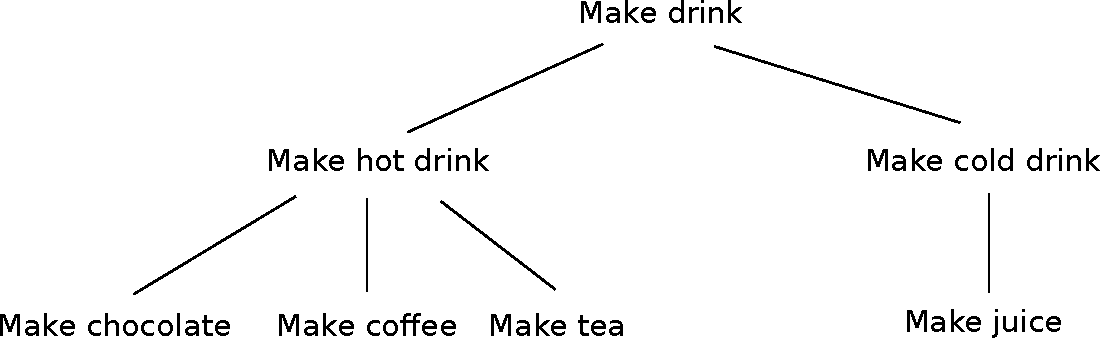
\includegraphics[width=\textwidth]{ADL_granularity.pdf}
    \caption{An example of ADL granularity represented as a tree.} 
    \label{fig-adl-granularity}
\end{figure}

To address different levels of activity granularity, ontological modelling, i.e. the process to explicitly specify key concepts and their properties for a problem domain, is applied. More concretely, ADLs are modelled as ontological concepts which are organised in a hierarchical structure in terms of their shared properties to form super-class and sub-class relations. Those relations between primitive and composite ADLs are characterised by ``is-a'' and ``part-of'' relationships, properly supported by OWL. For example, as shown in Figure \ref{fig-adl-granularity} making tea is a subclass of making hot drink. The ADL for making tea is represented by the ontological concept of MakeTea, while making hot drink is represented by MakeHotDrink. Properties establish the interrelations between concepts. For instance, \textit{hasDrinkType} is a property of the MakeHotDrink activity that links the DrinkType concept (e.g., tea, coffee, chocolate) to the MakeHotDrink concept. Both, concepts and properties, are modelled using the commonly shared terms in the problem community. The resulting ontologies are essentially knowledge models able to encode and represent domain knowledge and heuristics. 

The second feature of ADLs highlights the difference between generic and personalised ADLs. Even though making coffee implies the use of coffee and a container, some users prefer African coffee to Colombian coffee and some users use cups and others mugs. Furthermore, the order of the sequence of objects used to make coffee, vary from user to user, e.g. some users might add sugar before coffee and others add sugar once coffee has been poured to the container. In consequence, generic and personalised ADLs can be distinguished.

\begin{enumerate}
 \item Generic activity models: defined at the conceptual level as an activity class described by a number of properties. These properties describe the types of objects and their usage to perform an activity. Generic activity models are applicable to all users.
 \item Personalised activity models: they capture the specific way of a user to perform an activity and are modelled as instances of a corresponding conceptual activity model, which consists of specific information related to the concrete objects used and the sequential order they are used in.
\end{enumerate}

Activities are defined as ontological concepts and all actions that are required to perform the activity as the properties of the concept. For example, making tea involves taking a cup from the cupboard, putting a teabag into the cup, adding hot water to the cup, then milk and/or sugar. The ontological model of making tea, i.e. MakeTea concept, can be defined by action properties \textit{hasContainer}, \textit{hasTeabag}, \textit{hasHotwater}, \textit{hasMilk} and \textit{hasFlavour} in conjunction with descriptive properties such as activity start time \textit{actStartTime} and duration \textit{actDuration}. Notice that two kinds of properties are defined: \textit{action properties}, which refer to action-based properties and \textit{descriptive properties}, which are used to characterise the manner in which an activity is performed. This distinction is very important, because action properties play a crucial role for activity recognition. Indeed, activities are inferred from action properties which are generated by the sensor activations occurring due to human-object interactions. On the other hand, descriptive properties are not determinant in activity recognition. For instance, making coffee can happen at any time, it can be performed in different sequences and it may take variable amounts of time. As such, descriptive properties are used to model user's activity profiles, which are not used for the activity recognition process.

Hence, action properties define generic ADL models, which are used for activity recognition and are applicable to any user. Descriptive properties capture the different ways of performing generic ADLs, in terms of the objects used, the order in which those objects have been used, activity start time and duration. Personalised ADL models are instances of the corresponding generic ADL model.

In summary, ontological ADL modelling properly addresses different levels of activity granularity and the difference between generic and personalised ADLs, using the tools provided by markup languages such as OWL and RDF. 

\subsection{Ontological context modelling}

The ADL modelling scheme described above establishes a clear dependency between the context and an ADL. Indeed, ADLs are described as a set of context events, where context refers to temporal, spatial, event and environmental aspects. Exemplary temporal aspects of an ADL may be the start time and the duration of the activity, which are captured by descriptive properties. Spatial aspects relate to location information and surrounding entities such as rooms, household furniture and appliances. Event contexts capture dynamic state changes of the objects of the environment, for example, state changes of doors, fridge door or a microwave oven. Those events are modelled by action properties. Finally, environmental aspects of the context are composed of environmental information such as temperature, humidity and general weather conditions. 

In the dense sensing paradigm, contextual information is captured through various sensors. Each sensor monitors and reflects one facet of a situation. Based on this observation the context modelling is centred on ontological sensor modelling. Sensors are inherently linked to a number of physical and conceptual entities such as objects, locations and states. For example, a contact sensor is attached to a teapot in the second cupboard to the left of the sink in the kitchen. By explicitly capturing and encoding such domain knowledge in a sensor model it is possible to infer the corresponding objects and location from the activation of the sensor. This implies that a user performs an activity in the inferred location with the inferred object.

As most ADLs require the interlinking and fusion of data from multiple, disparate sensor sources in order to infer the high-level activities, it is necessary to aggregate a sequence of sensor activations to generate a situation at a specific time point. The situation formation process can be described as follows. Each sensor has a default state value for its state property, denoting the state of the object to which it is attached. When a sensor is activated, the state property will change. Subsequently the system will translate the state change as an occurrence of a user- object interaction at the specific time. As it is difficult, if not impossible, to monitor what happens at detailed levels after an object is interacted with, it is common practice to interpret a sensor activation as a user-object interaction, ignoring how the object is used and when it is de-activated. As such a user-object interaction is equivalent to an instantaneous sensor activation and can be interpreted as an object being used for performing an activity. In this way, by aggregating individual user-object interactions along a timeline the situation at specific time points can be generated. 

Under this context modelling approach, sensor activations are assumed to be produced by user-object interactions, which may denote an action property or a descriptive property, depending on the nature of the object and sensor. For example, a thermometer state change will be captured by a descriptive property such as \textit{hasTemperature(value)}, whereas a contact sensor installed in a cup will generate the action property \textit{hasContainer(cup)}. 

\subsection{Final remarks about ontology-based activity modelling}

A common framework to model ADLs and contextual information is provided by the ontology-based activity modelling approach described in \cite{Chen2012a}. Ontology-based activity modelling provides semantically clear, structured and reusable models. Furthermore, it offers a unified framework to combine generic models that can be applied to any user with personal models. By means of ontological modelling some traditional problems of data-driven approaches can be avoided, such as the manual class labelling, pre-processing and training processes. In addition, ontologies allow software agents to interpret data and reason against ontological contexts, thus enhancing the capabilities of automated data interpretation and inference.

However, the main problem of this modelling approach is related to model incompleteness. Obtaining complete models from domain knowledge for every person is not generally possible. An ADL model is composed by action and descriptive properties, so model incompleteness refers to the impossibility of completely defining all the action and descriptive properties of an ADL. In the case of descriptive properties, model incompleteness is obvious, since those properties refer to personalised ways of performing activities. Chen et al. propose in \cite{Chen2014} a hybrid activity modelling approach to learn descriptive properties from user generated data. But they assumed that ADL models in terms of action properties are complete. This assumption does not generally hold, because even though there are certain actions that every user performs for a given activity, there might be some other actions that cannot be known in the modelling step. 

Hence, this dissertation tackles the problem of learning unmodelled action properties for activity models. By means of learning new actions through incremental data-driven learning techniques, the static and generic nature of knowledge-driven activity models is also tackled. The contributions of this dissertation allow dynamic activity models which evolve in time and support both, generic and personalised models.
\section{Definitions and Constraints}
\label{sec:approach:def}

For the rest of the dissertation the following terms and concepts will be used according to the definitions provided in this section:

\begin{defn}[Sensor activation (SA)]
\label{def-sa}
 A sensor activation occurs when a sensor changes its state from the no-interaction state to interaction state. Reverse transitions, i.e. de-activations of sensors, are not considered. For example, when a user takes a glass, the activation is tagged as \textit{glassSens}. A sensor activation is then composed by a time-stamp and a sensor identifier:
 
 \begin{equation}
  SA = \{ time-stamp, sensorID \}
 \end{equation}

\end{defn}

\begin{defn}[Sensor activation dataset]
\label{def-sa-dataset}
 A time-ordered sequence of sensor activations.
\end{defn}

\begin{defn}[Actions]
\label{def-action}
 Actions are the primitives of activities and are directly linked to sensor activations. For example, the activation of sensors \textit{cupSens} and \textit{glassSens} are linked to the action \textit{hasContainer}. A sensor activation can only be mapped to one single action, but an action can be generated by different sensor activations. Actions do not have any duration and are hence described by a time-stamp.
\end{defn}

\begin{defn}[Type]
\label{def-type}
 When referring to activities and objects, type captures a purpose based classification. In this dissertation, considered types are \textit{Cooking}, \textit{Hygiene}, \textit{Entertainment} and \textit{Housework}. An activity can only have one type, while objects can have more than one. For example, an object like a tap can be used for cooking, housework or hygiene. But a MakeCoffee activity can only be a cooking activity. On the other hand, when referring to sensors, type classifies sensors in terms of their technological base. In this dissertation, modelled sensor types are \textit{contact}, \textit{electric}, \textit{pressure} and \textit{tilt} sensors. 
\end{defn}

\begin{defn}[Location]
\label{def-location}
 Location refers to semantic places of the monitored environment, where sensor activations occur and hence, activities are performed. For example, in a house, possible locations might be \textit{bedroom}, \textit{bathroom} or \textit{kitchen}. 
\end{defn}

\begin{defn}[Initial Activity Model (IAM)]
\label{def-iam}
Activity models are sequences of actions defined by a domain expert. Initial activity models refer to the minimum number of necessary actions to perform an activity. The objective of such models is to represent incomplete but generic activity models applicable to any user. Initial activity models also have an estimation of the maximum duration of the activity.
\begin{equation}
  IAM(Activity_n) = \{action_a, action_b, \ldots , max\_duration\}
 \end{equation} 
\end{defn}

\begin{defn}[Extended Activity Model (EAM)]
\label{def-eam}
 A complete and specialised version of an IAM. By \textit{complete} we mean that an activity model contains all the actions performed by a user for the corresponding activity. By \textit{specialised} we mean there are two or more different complete action sequences for the corresponding activity, i.e. specialised sub-classes of that activity exist. The EAM for an activity is represented as a list of action sequences with their occurrence frequency:
\begin{equation}
 \begin{split}
 EAM(Activity_n) = \{as_1, as_2, \ldots , as_n\} \ \ \ where \\
 as_i = \{frequency, action_a, action_b, \ldots, action_m\}
 \end{split}
 \label{eq-eam}
\end{equation}
\end{defn}

\begin{defn}[User Erratic Behaviour]
\label{def-erratic}
 When a user interacts with an object but the interacted object is not being used to perform the ongoing activity. Consider the case where a user wants to prepare pasta. In order to take the pasta from the store, the sugar package has to be removed first. The user will touch the sugar package and thus, a sensor activation will be generated. But this interaction does not mean that sugar is being used to prepare pasta. 
\end{defn}


\begin{defn}[Positive Sensor Noise]
\label{def-positive}
 A sensor that should not get activated, i.e. there is no interaction with the object monitored by the sensor, gets activated because of sensor or monitoring infrastructure errors.
\end{defn}

\begin{defn}[Missing Sensor Noise]
\label{def-missing}
 A sensor that should get activated, i.e. there is an interaction with the object monitored by the sensor, does not get activated because of sensor or monitoring infrastructure errors.
\end{defn}



The learning approach for activity models presented in this dissertation has some constraints:

\begin{cons}[Dense sensing-based activity monitoring]
\label{cons-dense}
 Even though there is no theoretical constraint that prevents the approach to be implemented for other activity monitoring approaches, the implementation presented in this dissertation is designed for the dense sensing-based activity monitoring approach.
\end{cons}

\begin{cons}[Single user - single activity scenario]
\label{cons-single}
 This is a hard constraint, in the sense that the theoretical foundations of the learning approach assume explicitly that only one user is being monitored and this user is not allowed to perform concurrent or interleaving activities.
\end{cons}

\begin{cons}[Uniquely located activities]
\label{cons-location}
 It is assumed that an activity can only be performed in a single location, during a concrete execution, i.e. although ReadBook can be performed in the bedroom and in the lounge, a concrete execution will take place in the bedroom or in the lounge (exclusive or).
\end{cons}

\begin{cons}[``Static'' objects]
\label{cons-static-obj}
 Objects used by a user are assumed to be ``static'' respect to the location, i.e. if the location of a brusher is the bathroom, the object will always stay in the bathroom.
\end{cons}
\section{Solution Design}
\label{sec:approach:solution}

Based on the definitions and constraints shown in Section \ref{sec:approach:def}, an offline system for extended activity model learning is presented. The objective of the system is to learn extended activity models (EAM, definition \ref{def-eam}) for every defined activity and a particular user, since every user has his/her own way to perform activities in terms of executed actions. The initial activity models (IAM, definition \ref{def-iam}) for every activity provided by a domain expert will be the same for every user, because they are generic models. But the extended activity models are personal models. They capture different complete activity models performed by a user. Notice that EAM learning has several implications in the ontology-based activity model approach:

\begin{enumerate}
 \item Complete models are learnt for every activity and a particular user. Complete refers to the sequence of executed actions for a concrete activity.
 \item If two or more different complete models are learnt for a concrete activity, specialised models of the same activity are found. This means that the defined activity is not a leaf in the ADL ontological tree and hence, sub-activities of that activity are discovered.
 \item Activity models can be dynamic. If the EAM learning system is continuously updated with new data, activity models can be updated. In consequence, activity models evolve and are adapted to users' varying behaviours.
\end{enumerate}

\subsection{Inputs of the learning system}
\label{subsec:approach:inputs}

The learning system for EAMs works on user generated data. It combines domain knowledge and user generated data in a learning algorithm. Notice that user data comes in an unlabelled sensor activation dataset, so there is no need to manually label any dataset. On the other hand, domain knowledge concerning the environment and activities is provided to the learning system. More concretely, the inputs of the EAM learning system are:

\begin{enumerate}
 \item Context knowledge: the context knowledge represents the prior knowledge provided by a domain expert which is relevant to learn activity models. The concepts modelled in the context knowledge include: 
 \begin{enumerate}
  \item Activities: every activity is defined by its name, type, location and IAM. Following definition \ref{def-type}, an activity has only one type. However, an activity can be performed in several locations (notice that this does not contradict constraint \ref{cons-location}). 
  \item Objects: objects refer to every object in the environment which are monitored by sensors and are used to perform activities. An object is defined by its name, type, location and attached sensors. As definition \ref{def-type} states, an object can have several types. But an object is subjected to constraint \ref{cons-static-obj}, so it has a unique location. In principle, objects can be monitored by several sensors. For instance, a fridge may have a tilt sensor attached to its door to monitor open/close door action and a electric sensor to monitor the power usage.
  \item Sensors: following constraint \ref{cons-dense}, sensors are attached to objects and they are defined by a sensor identifier, type, described action and object to which it is attached. Sensors produce sensor activations (definition \ref{def-sa}) when they transition from their no-interaction state to interaction state. Sensors have a unique type and they are mapped to one single action, as stated in definition \ref{def-action}. The object to which the sensor is attached is also stored in the context knowledge.
 \end{enumerate}
 
 \item Sensor activation dataset: as defined in definition \ref{def-sa-dataset}, an unlabelled time-stamped sensor activation dataset with the activity traces of a concrete user.
\end{enumerate}

In the current implementation, context knowledge is formatted in a JavaScript Object Notation (JSON)\footnote{http://json.org/} file. JSON has been selected because it provides a light-weight knowledge formatting syntax which is widely supported and used to share information. Although OWL or RDF could be used to implement context knowledge, the overhead introduced by such markup languages comes without any advantage for the EAM learning system. The decision of using JSON responds to the principle of providing a simple solution, focusing on modelling only relevant knowledge. As an example, Figure \ref{fig-context-json} shows how an activity, an object and a sensor are modelled in the context knowledge file. This knowledge is provided by a domain expert and modelled by knowledge engineers. 

\begin{figure}[htbp]
\begin{small}
\begin{lstlisting}
"MakeCoffee": {
	"type": ["Cooking"],
	"location": ["Kitchen"],
	"IAM": ["hasContainer", "hasCoffee"],
	"duration": 300
}
---------------------------------------------------
"kitchen-tap": {
	"type": ["Cooking", "HouseWork"]
	"location": "Kitchen"
	"sensors": ["ktapSens"]
}
---------------------------------------------------
"ktapSens": {
	"type": "tilt",
	"action": "turnOnTap",
	"attached-to": "kitchen-tap"
}
\end{lstlisting}
\end{small}
\caption{Example of activities, objects and sensors modelled in the context knowledge file. Activity duration is given in seconds.}
\label{fig-context-json}
\end{figure}

The second input to the EAM learning system is the sensor activation dataset. For the implementation presented in this dissertation, sensor activation datasets are formatted in Comma Separated Value files (CSV)\footnote{http://en.wikipedia.org/wiki/Comma-separated\_values}. Each row of the file contains a time-stamp (year, month, day and time) and a sensor activation tagged with the sensor identifier which has produced the activation (see Figure \ref{fig-dataset}).


\begin{figure}[htbp]
\begin{small}
\begin{lstlisting}
2014-05-23 09:47:33.984341,storeSens
2014-05-23 09:47:39.333528,potSens
2014-05-23 09:47:52.750216,cookerSens
2014-05-23 09:48:07.764138,fridgeSens
2014-05-23 09:48:12.591836,wmilkSens
2014-05-23 09:48:47.199512,chocoSens
2014-05-23 09:54:11.553695,mugSens
2014-05-23 09:54:40.794979,rcontrolSens
2014-05-23 09:54:50.390696,tvSens
2014-05-23 09:54:59.348862,sofaSens
\end{lstlisting}
\end{small}
\caption{A slice of a sensor activation dataset.}
\label{fig-dataset}
\end{figure}

Based on those inputs, a context knowledge file and a sensor activation dataset, the output of the EAM learning system is a list of action sequences for each activity, which describe the EAMs for each activity (see equation \ref{eq-eam}). 

\subsection{Intuition behind the solution}
\label{subsec:approach:intuition}
The intuition for the designed solution to EAM learning comes when sensor activations are plotted in a three-dimensional space spanned by location, type and time, as shown in Figure \ref{fig-action-plot}. This three-dimensional space, named activity space, reflects the prior knowledge about activities. An activity has a concrete type that is shared with the object types used to perform that activity and is performed in a location and a time segment. 

\begin{figure}[htbp]
\centering
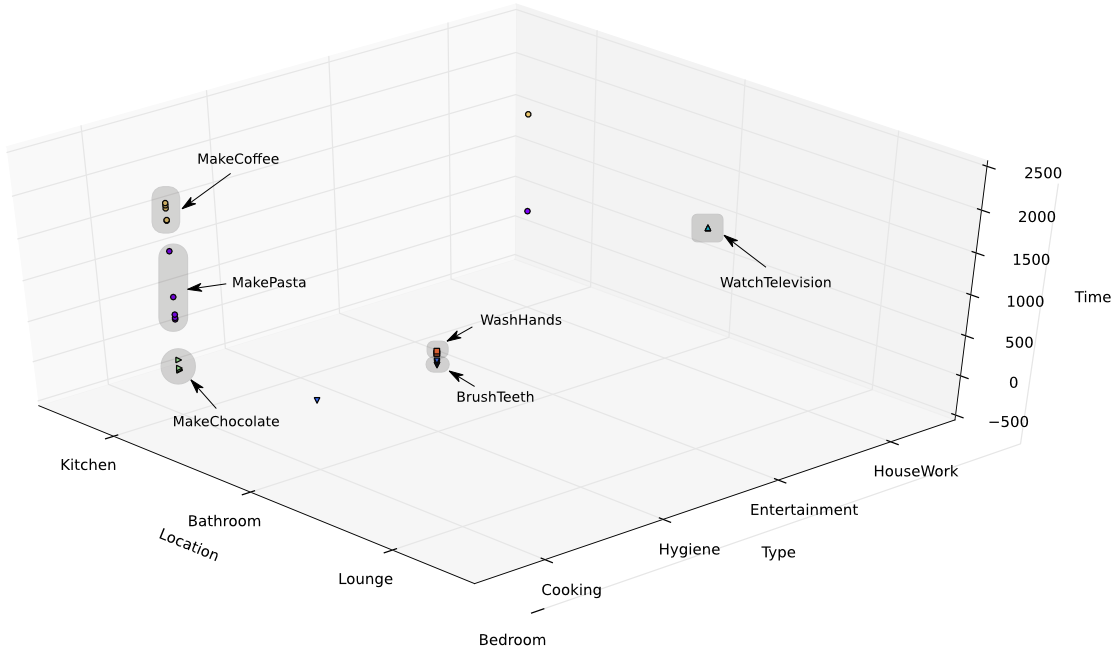
\includegraphics[width=\textwidth]{activity_visualization_m.png}
    \caption{A plot of the actions executed by a user for performing several activities in the three-dimensional space spanned by location, type and time.}
    \label{fig-action-plot}
\end{figure}

When sensor activations describing several activities are plotted in the activity space, several lumps or clusters can be distinguished. Intuition says that sensor activations, and hence actions, have to be close to each other when they form an activity (close in the activity space), i.e. if a user is making pasta, it is common sense to think that sensor activations describing that activity will be located in the kitchen, and the objects which are being used by the user will be for cooking purposes. As far as time regards, sensor activations will occupy a time segment which will denote the duration of the activity.

This grouping of actions in the activity space can be seen in Figure \ref{fig-action-plot}. Six activities can be identified there, namely MakeChocolate, BrushTeeth, WashHands, MakePasta, MakeCoffee and WatchTelevision. Due to time resolution in the graphic, actions composing BrushTeeth, WashHands and WatchTelevision cannot be properly distinguished. Those three activities are quite short in time, but depicted actions for each of them are respectively five, three and three. There are some actions that are not grouped in any activity. Those actions are generated by objects that have multiple types. For example, in the case of MakePasta, the kitchen tap is used. The kitchen tap can be used for cooking or for housework and that is why it appears in both positions.

It is interesting to see how Figure \ref{fig-action-plot} supports the intuition about action distribution in the activity space. In general, actions can be easily grouped in activities, but there are also some tough cases. This is the case of actions composing activities BrushTeeth and WashHands, which are very close in time and are performed in the same location and with the same purpose. The last action of MakePasta seems also difficult to group, since it is closer in time to activity MakeCoffee, sharing again the same location and type. 

In consequence, the idea is to design a clustering algorithm which takes advantage of location, type and time information to aggregate actions to clusters. The clustering process needs heuristics and metrics that take special care of those actions that are difficult to group in the corresponding activity. But this is not enough. Activity clusters have to be identified and labelled with one of the defined activities. To identify action clusters with activity names, initial activity models in the context knowledge can be used. Initial activity models contain an incomplete sequence of actions. Despite being incomplete sequences, they can be used to identify activities. So the clustering algorithm has to produce several labelled action/sensor activation sequences per activity.

The clusters extracted in the clustering process may contain all the actions executed by a user to perform a concrete activity. Those clusters may be used to learn different ways of performing an activity and hence, to learn extended activity models. In summary, the key idea is to design a clustering algorithm that uses initial activity models to detect activities and some metrics in the activity space to aggregate actions to activities. Afterwards, using the clusters extracted and labelled, analyse them to learn extended activity models for each activity.

%To learn those models a two-step system is presented. First, a clustering process is run in the so called \textbf{semantic space of actions}, using initial activity models to label each cluster with a modeled activity. The semantic space of actions is a three-dimensional space spanned by the axes of location, type and time. Actions carried out by a user have only one location in the environment (bathroom, kitchen etc.), one time instant, but multiple types. For instance, a glass can be used for multiple activity types, such as cooking, eating or personal hygiene (brushing teeth). Hence, the action \textit{hasContainer} linked to a glass activation, occupies multiple positions in the type axis. 

\subsection{Description of the solution}
Following the intuition described in section \ref{subsec:approach:intuition}, a solution for the EAM learning system has been designed. The adopted system architecture is depicted in Figure \ref{fig-design}. In a first glance, the two important blocks identified in section \ref{subsec:approach:intuition} can be distinguished in the architecture: a clustering process and an activity model learning process. The clustering process is implemented in two modules, namely the Semantic Activity Annotation module ($SA^3$) and the Action Aggregator module ($AA$). On the other hand, the activity learning process is implemented by a module called Activity Model Learner ($AML$). 

\begin{figure}[htbp]
\centering
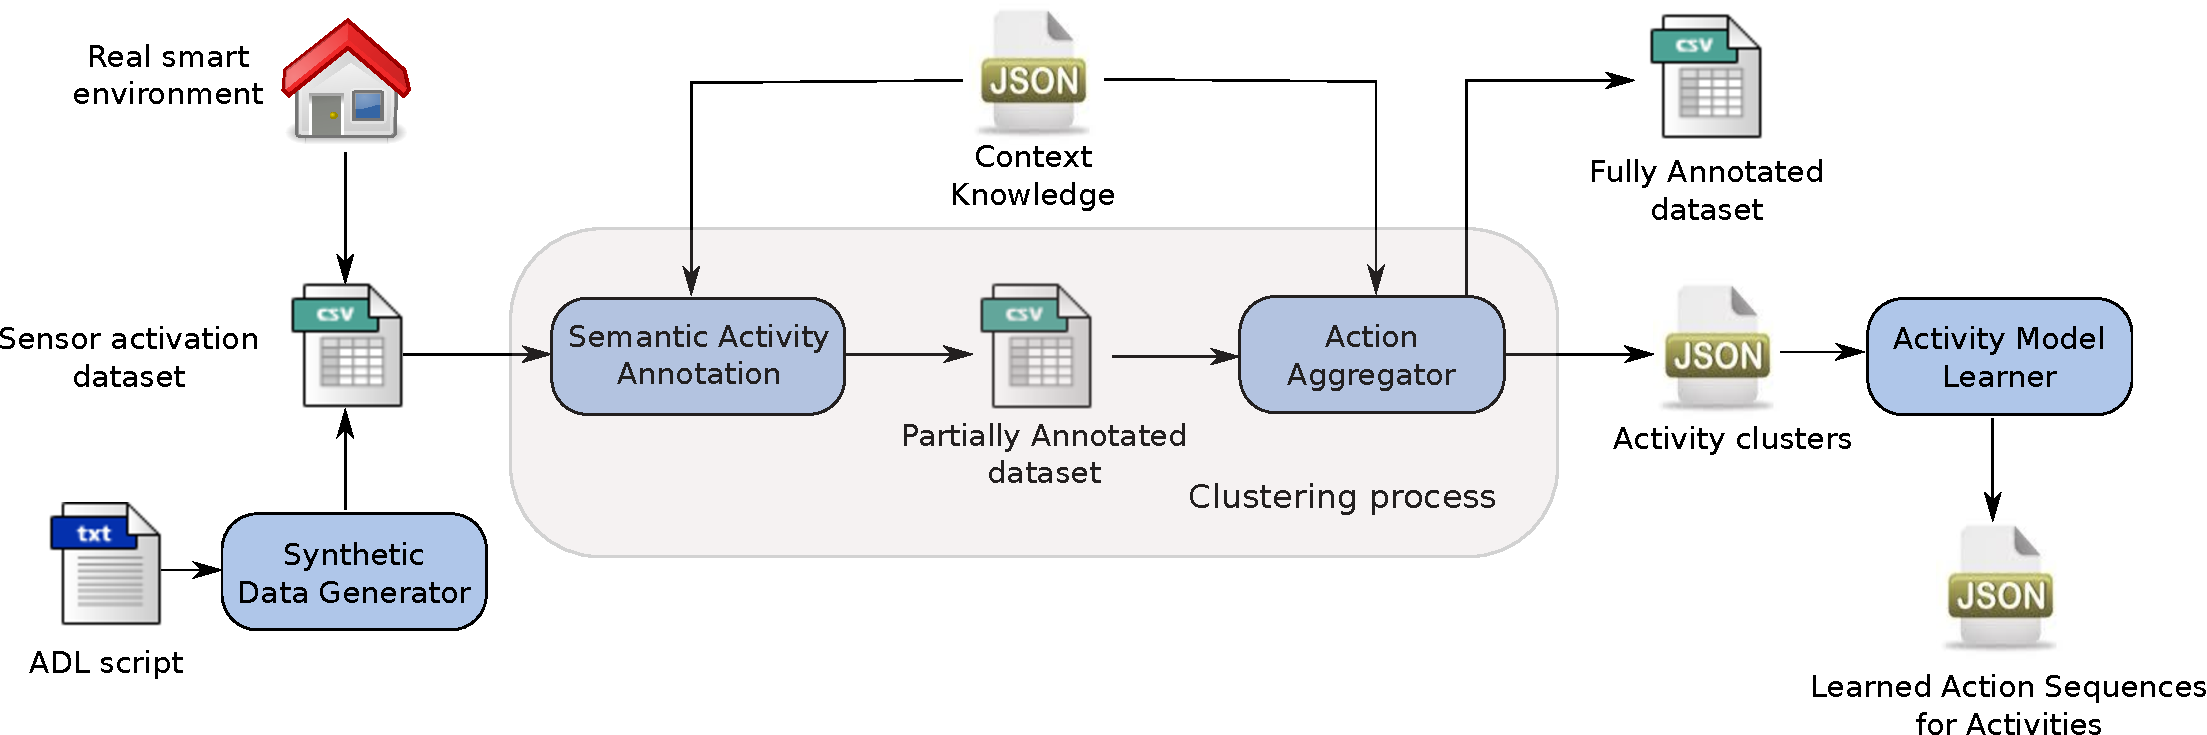
\includegraphics[width=\textwidth]{our_approach.pdf}
    \caption{The detailed design architecture of the proposed approach to learn EAMs.}
    \label{fig-design}
\end{figure}

Two kinds of elements can be distinguished in the architecture depicted in Figure \ref{fig-design}: files and software modules. The only exception to this rule is the \textit{real smart environment}, which represents a sensorised environment where a user performs several activities. All the other elements can be classified into files or software modules. There are three kinds of files: plain text files (\textit{ADL script}), JSON files (\textit{context knowledge}, \textit{activity clusters} and \textit{learned action sequences for activities}) and CSV files (\textit{sensor activation dataset}, \textit{partially annotated dataset} and \textit{fully annotated dataset}). Files are used to exchange information between software modules. The developed software modules are four: \textit{Synthetic Data Generator}, \textit{Semantic Activity Annotation}, \textit{Action Aggregator} and \textit{Activity Model Learner}. All the software modules of the diagram have been implemented using Python 2.7\footnote{https://www.python.org/} and its packages Numpy\footnote{http://www.numpy.org/} for numerical computing and Pandas\footnote{http://pandas.pydata.org/} for data analysis. 

Once the elements of the architecture have been described, the solution itself will be detailed. Firstly, a sensor activation dataset has to be collected for a concrete user. A real smart environment or a synthetic data generator can be used to get this dataset. The sensor activation dataset contains all sensor activations registered for a user performing certain activities during a fixed period of time. Remember that sensor activations are unlabelled. Whatever method has been chosen to obtain it, the resulting sensor activation dataset is formatted in a CSV file and its information has already been defined in definition \ref{def-sa-dataset}.

Afterwards, a novel clustering process is run on the sensor activation dataset, using the context knowledge provided by an expert and formatted in a JSON file. The proposed clustering process, which is extensively discussed in Chapter \ref{cha:clustering}, is divided into two steps: 

\begin{enumerate}
 \item Semantic Activity Annotation algorithm ($SA^3$): this algorithm uses IAMs stored in the context knowledge to detect activities in the unlabelled dataset. It transforms sensor activations to actions according to context knowledge to apply a novel pattern recognition algorithm that has been designed and implemented to detect the occurrence of IAMs in the unlabelled sensor activation dataset. $SA^3$ also uses object and activity location information to infer from sensor activations where an activity is being performed and analyse consequently the feasibility of the detected pattern. $SA^3$ is an initialisation process from the clustering point of view, because it finds initial clusters in the time axis and identifies the label of those clusters. The output of $SA^3$ is given in the so called \textit{partially annotated dataset}, where sensor activations and their resultant actions are labelled with activity names or the special label 'None', which indicates that the action could not be labelled with any known activity name. Notice that $SA^3$ only labels those actions that pertain to IAMs thus leaving the vast majority of actions without any label. This is the reason why the output of the algorithm is called \textit{partially annotated}. A detailed description of $SA^3$ is given in Section \ref{sec:clustering:sa3}.
 \item Action Aggregator algorithm ($AA$): the input to the algorithm is the output of $SA^3$, i.e. the partially annotated dataset file. $AA$ uses activity, object and action knowledge described in the context knowledge to expand initial activity clusters detected by $SA^3$. To analyse those actions that remain unlabelled after $SA^3$, $AA$ defines boolean functions based on location, type and time information of actions and objects. It analyses unlabelled actions that are close to initial clusters, checking the feasibility of those actions pertaining to those close initial clusters. The feasibility is computed using location, type and time information, implementing the idea that actions pertaining to an activity are performed in the same location, with a coherent purpose and close in time. $AA$ algorithm's result is stored in another CSV file called \textit{fully annotated dataset}, which assigns an activity label to all actions and their original sensor activations. The special label 'None' is used for those actions that are not considered part of any activity. Those actions can be originated by sensor noise or user erratic behaviour, i.e. a user that interacts with an object that is not being used for performing an activity. Additionally, $AA$ also generates a JSON file called \textit{activity clusters}. This file contains all the clusters found by the algorithm for each activity. Clusters, which are action sequences, come with an occurrence frequency. The activity clusters file is also used to store some interesting statistics found by $AA$ about the frequency of objects used and actions executed for each activity, frequency of locations in where each activity has been performed and activity duration statistics (mean and standard deviation). An example of an activity clusters file can be seen in Figure \ref{fig-clusters-file}. $AA$ algorithm is described in Section \ref{sec:clustering:ac}.
\end{enumerate}

\begin{figure}[htbp]
\begin{small}
\begin{lstlisting}
    "ReadBook": {
        "locations": [
            [42, "Bedroom"], 
            [11, "Lounge"]
        ], 
        "actions": [
            [53, "useFurniture"], 
            [53, "turnOnLamp"], 
            [53, "hasBook"]
        ], 
        "patterns": [
            [
                53, 
                [
                    "useFurniture", 
                    "turnOnLamp", 
                    "hasBook"
                ]
            ]
        ], 
        "objects": [
            [42, "bed"], 
            [42, "bedroom-lamp"], 
            [42, "book-b"], 
            [11, "sofa"], 
            [11, "lounge-lamp"], 
            [11, "book-a"]
        ], 
        "occurrences": 53, 
        "duration": [
            14.773584905660377, 
            2.6467602797835856
        ]
    }, 
\end{lstlisting}
\end{small}
\caption{Information stored in an activity clusters file for activity ReadBook.}
\label{fig-clusters-file}
\end{figure}

The main result of the clustering process is thus stored in the activity clusters JSON file. Activity clusters have the information of all action sequences executed by a user to perform a concrete activity. For example, in the file shown in Figure \ref{fig-clusters-file}, in the ``patterns'' section, all the action sequences found by $AA$ are stored. In this case, for activity ReadBook, only one cluster has been generated with 53 occurrences in the sensor activation dataset. According to $AA$, ReadBook has been performed by means of executing the action sequence \textit{useFurniture}, \textit{turnOnLamp} and \textit{hasBook}. Nevertheless, $AA$ generally finds many different clusters per activity. Those clusters are finally processed by Activity Model Learner ($AML$), which filters incorrect action sequences and outliers to learn final EAMs as a list of action sequences. $AML$ uses action sequence similarity metrics to implement a novel outlier detection. Notice that all action sequences or clusters detected by $AA$ are not valid action models, since they may contain incorrectly labelled actions (due to clustering errors, sensor errors and/or user erratic behaviour) and missed actions (due to sensor errors). Those spurious action sequences have to be detected and removed, to discover those action sequences that are valid models for a given activity. Valid action sequences are the EAMs for activities and are stored in a JSON file called \textit{learned action sequences for activities}. All the details about $AML$ are provided in Chapter \ref{cha:learner}.
\section{Summary and Conclusions}
\label{sec:clustering:sum}

%: ----------------------- clustering process ------------------------

% this file is called up by thesis.tex
% content in this file will be fed into the main document

%: ----------------------- introduction file header -----------------------
\begin{savequote}[50mm]
If I have seen further it is by standing on the shoulders of giants.
\qauthor{Isaac Newton}
\end{savequote}

\chapter{Related Work}
\label{cha:soa}

% the code below specifies where the figures are stored
\ifpdf
    \graphicspath{{2_state_of_the_art/figures/PDF/}{2_state_of_the_art/figures/PNG/}{2_state_of_the_art/figures/}}
\else
    \graphicspath{{2_state_of_the_art/figures/EPS/}{2_state_of_the_art/figures/}}
\fi

%\letra{D}{escribe} how the state of the art has been structured in this chapter, referencing sections and commenting on their contents. Justify the topics covered by the chapter.

\letra{H}{uman} activity recognition is a broad research area which can be analysed from many different points of view. The objective of this chapter is to provide a high-level picture of the current status of the research topic, to then describe more in detail the concrete approaches that are related to the work presented in this dissertation. 

First of all, Section \ref{sec:soa:har} introduces the concept of \textit{Human Activity Recognition}, shows its main applications and provides a high-level taxonomy of activity recognition approaches. Section \ref{sec:soa:sensor} describes in detail the category in which this dissertation fits regarding the monitoring approach: \textit{Sensor-Based Activity Recognition}. Based on the specific sensors used for activity monitoring, Section \ref{sec:soa:monitoring} presents a more detailed taxonomy for the category of sensor-based activity recognition. On the other hand, the following sections analyse the main currents of activity modelling, which is the focus of this dissertation: Section \ref{sec:soa:datadriven} presents \textit{Data-Driven Approaches}, while Section \ref{sec:soa:knowledgedriven} describes in detail \textit{Knowledge-Driven Approaches}. A summary and comparison of both activity modelling currents is provided in Table \ref{tab:soa:comparison}. Some recent work has settled the basis to combine both currents, giving as result the \textit{Hybrid approaches}, as shown in Section \ref{sec:soa:hybrid}. This dissertation is another step in order to achieve hybrid approaches that can combine effectively the best features of knowledge- and data-driven approaches. The chapter finalises with Section \ref{sec:soa:summary}, where a concise summary is provided alongside with some conclusions.
\section{$SA^3$: Semantic Activity Annotation}
\label{sec:clustering:sa3}

%Brief introduction to the algorithm:
%- Inspired in knowledge-driven techniques, specially in Chen's work
%- It is not activity recognition, but offline annotation
The annotation algorithm presented in this paper is inspired in knowledge-driven activity recognition methods, specially in \cite{Chen2012a}. Three important concepts from that work are extracted and used for the presented approach:

\begin{itemize}
 \item \textbf{Domain knowledge allows recognizing activities reliably:} in contrast with data-driven techniques, which use intensively annotated datasets in order to learn activity models for recognition, knowledge-driven techniques use expert domain knowledge to model activities. Those models can be reliably used for activity recognition
 \item \textbf{Sensor activations are linked to user-object interactions:} if a contact sensor installed in a cup changes its state, the object is assumed to be used for an activity. Sensors' information is modelled to allow transformations from sensor activations to user-object interactions or \textbf{actions}. Following with the contact sensor of the cup, whenever an activation is received, it is interpreted as an action, which can be named as \textit{hasContainer(cup)}
 \item \textbf{Activities can be modelled as sequences of actions:} even though richer information can be provided as location and time, to keep activity models as simple as possible, we only consider necessary actions. As such, the \textit{MakeCoffee} activity can be modelled as the action sequence \textit{\{hasContainer(x), hasCoffee(y)\}}.
\end{itemize}

Real-time activity recognition needs complete activity models to have a reliable recognition performance. However, providing complete activity models is very complicated, since each user executes varied action sequences to perform the same activity. For example, to make a coffee, some users may use milk and sugar, while others may add only some cream. But making coffee will always imply using coffee and having a container, i.e. the action sequence \textit{\{hasContainer(x), hasCoffee(y)\}}. This prior knowledge is used in $SA^3$ for activity annotation.

Activity annotation and recognition is not the same thing. Activity annotation can make use of the whole dataset offline, with no time restrictions. On the other hand, activity recognition is required to work while activities are being performed, so only past sensor activations can be used. This key difference makes feasible using incomplete activity models to annotate activities, in contrast with the real-time recognition problem.

\subsection{Basic Concepts}
%- Explain what sensor activations and actions are (ontologies could be good to represent that knowledge, but we do not use them at this moment to make the tool lighter)
%- Explain minimal activity models (action patterns + maximum duration) (once again, ontology issues)
%- Time-stamped sensor activation dataset (show a sample and explain)
\begin{itemize}
 \item \textbf{Sensor activations (SA):} it is assumed that environments are equipped with sensors that can collect information about user-object interactions. Whenever those sensors change their states, a sensor activation is collected. Sensor activations are then composed by a sensor identifier and a time-stamp
 \begin{equation*}
  SA = \{time\text{-}stamp, sensorID\}
 \end{equation*}
 \item \textbf{Sensor dataset:} a time-ordered sequence of sensor activations
 \item \textbf{Actions:} actions are the primitives of activities and are directly linked to sensor activations. The link between sensor activations and actions is manually established. Tables are used where several sensor activations are linked to an action. For example, \textit{cupObjSensor} and \textit{glassObjSensor} are linked to the action \textit{hasContainer}. A sensor activation can only be linked to one single action. The transformation function is defined as:
 \begin{equation*}
  Trans(SA) : SA \rightarrow Action
 \end{equation*}

 \item \textbf{Action dataset:} a time-ordered sequence of actions
 \item \textbf{Minimal activity models:} activity models are sequences of actions defined by a domain expert. Minimal activity models refer to the minimal number of necessary actions to perform an activity. The objective of such models is to represent incomplete but generic activity models which provide enough information to detect activities. Minimal activity models also have an estimation of the maximum duration of the activity based on a heuristic %That duration estimation turned to be essential for robust annotation in noisy scenarios
 \begin{equation*}
  Activity_n = \{action_a, action_b, \ldots , max\_duration\}
 \end{equation*}

\end{itemize}


\subsection{$SA^3$: Semantic Activity Annotation Algorithm}
%- Maybe having a name for the tool could be nice -> SA3 ?
%- Explain the three-step algorithm
%- Show pseudo-code for the algorithm

Having as inputs a sensor dataset, sensor-action transformation functions and minimal activity models, the objective of $SA^3$ is to generate an annotated sensor dataset, where each sensor activation will have an activity label or the special label \textit{None}, which represents lack of known activity. Single-user single-activity scenarios are considered, so no interleaved activities will be in the sensor dataset. Considering those constraints, a three-step algorithm has been designed:

\begin{enumerate}
 \item \textbf{Sensor-action transformation step:} the first step takes as input the sensor dataset and transformation functions to generate an action dataset. For each sensor activation in the sensor dataset, the transformation function is applied to obtain the corresponding action. In consequence, a sensor sequence such as:
 \begin{equation*}
 \begin{split}
   \{cupObjSensor, whiteSugarSensor, skimmedMilkSensor\}
 \end{split}  
 \end{equation*}
 will be transformed to:
 \begin{equation*}
 \begin{split}
  \{hasContainer(cup), hasFlavour(white\text{-}sugar), hasMilk(skimmed\text{-}milk)\}
 \end{split}   
 \end{equation*}
 
Since only actions and not objects are relevant for activity annotation, \textit{hasContainer(cup)} will be used as \textit{hasContainer} 

 \item \textbf{Activity sequence finding step:} all the occurrences of minimal activity models are found iterating on the action dataset. For an action pertaining to a minimal activity model following actions are searched. Those actions are considered to describe the activity if two criteria are fulfilled: 
 \begin{enumerate}
  \item \textit{Completion criterion}: the action sequence has to contain all the actions of the corresponding minimal activity model
  \item \textit{Duration criterion}: the duration of the action sequence has to be smaller than the duration estimation of the corresponding minimal activity model
 \end{enumerate}
 Depending on the activity models, the actions dataset and noise levels, detected activities can overlap each other. Here is an illustrative example, where time-stamps are ignored since duration criterion is satisfied. Imagine we define minimal activity models for \textit{MakeCoffee, MakeTiramisu, MakeWhippedCream} and \textit{BrushTeeth}, where:
 \begin{equation*}
  \begin{split}
   MakeCoffee =\{hasCoffee, hasContainer, hasFlavour\} \\
  MakeTiramisu = \{hasCream, hasContainer, hasCoffee\} \\
  MakeWhippedCream = \{hasFlavour, hasContainer, hasCream\} \\
  BrushTeeth = \{hasBrusher, hasToothPaste, turnOnTap\} 
  \end{split}
 \end{equation*} 
 
Let us consider the following action sequence from the action dataset:
\begin{equation*}
\begin{split}
 \{hasContainer, hasCream, useCookingUtensil, hasFlavour, hasBrusher, \\ 
 hasCoffee, hasToothPaste, hasContainer, turnOnTap\}
\end{split}  
\end{equation*}
Figure \ref{fig:overlap} shows all the activities found applying the completion and duration criterion. Activities overlap each other, because there are several actions that belong to several activities. Notice also that there are some actions that are not in any activity model, which is totally feasible for our approach.
\begin{figure}[htbp]
\centering
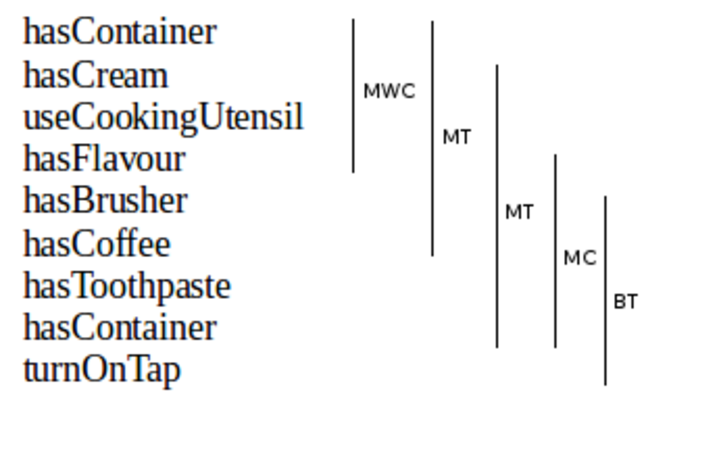
\includegraphics[width=\textwidth]{overlapping_activities.pdf}
    \caption{Illustrative example of the output of the step 2 of $SA^3$. MWC refers to \textit{MakeWhippedCream}, MT to \textit{MakeTiramisu}, MC to \textit{MakeCoffee} and BT to \textit{BrushTeeth}}
    \label{fig:overlap}
\end{figure}

\item \textbf{Correct activity sequence fitting step:} having the overlapping activities, the objective of this step is to find the maximum number of activities that do not overlap. This heuristic is derived from the fact that only none interleaved activities are considered. Applying it, the example of Figure \ref{fig:overlap} can be solved appropriately. The solution found by the algorithm is that there are only two activities in that action sequence:
\begin{equation*}
  \begin{split}   
  MakeWhippedCream = \{hasContainer, hasCream, useCookingUtensil, hasFlavour\} \\
  BrushTeeth = \{hasBrusher, hasCoffee, hasToothPaste, hasContainer, turnOnTap\} 
  \end{split}
 \end{equation*}  

Hence, \textit{hasCoffee} is probably due to a faulty sensor activation and \textit{hasContainer} may refer to a glass used in the bathroom to rinse the mouth. 
\end{enumerate}

This three-step algorithm is depicted as pseudo-code in Algorithm \ref{alg:sa3}. It has been designed to work with noisy sensor activations, varying order for activity executions and sensor activations that do not belong to any activity model. That flexibility allows using the tool in many different datasets. Section \ref{evaluation} contains many cases to show the performance of the algorithm in several demanding situations.

\begin{algorithm}
 \caption{$SA^3$ algorithm for semantic activity annotation}
 \label{alg:sa3}
 \begin{algorithmic}
 \REQUIRE sensor\_dataset, transformation\_function, minimal\_activity\_models
 \ENSURE annotated\_dataset
 \STATE $action\_dataset \leftarrow apply\_transform\_function(sensor\_dataset, transformation\_function)$
 \FORALL{$action \in action\_dataset$}
  \IF{$action \in minimal\_activity\_models$}    
    \STATE $activities \leftarrow obtain\_activities(action, minimal\_activity\_models)$
  \ENDIF
  \FORALL{$activity \in activities$}
    \STATE $// \text{ Use duration and completion criteria}$
    \STATE $detected\_activities \leftarrow find\_proper\_activities(minimal\_activity\_models)$
  \ENDFOR
 \ENDFOR
 \STATE $annotated\_dataset \leftarrow find\_non\_overlapping\_activities(detetected\_activities)$
 \RETURN $annotated\_dataset$
 \end{algorithmic}
\end{algorithm}

\section{AC: Activity Clustering}
\label{sec:clustering:ac}

Initial clusters provided by $SA^3$ are expanded in this step, using context knowledge and time-based metrics for action aggregation. The inputs of the $AC$ algorithm are the context knowledge file (see Section \ref{sec:approach:solution} and specially Figure \ref{fig-context-json}) and the partially annotated dataset returned by $SA^3$ (see Figure \ref{fig-partially-annotated}). The output of $SA^3$ is interpreted as the initialisation of the clustering process in the activity space spanned by location, type and time axis. $SA^3$ has been designed to provide the number of clusters in the dataset, their semantic label and their centroids in the time axis. Having this initialisation, $AC$ is the responsible of analysing all actions considering the three dimensions of the activity space and deciding which actions are aggregated to the initial clusters provided by $SA^3$.

Assume Figure \ref{fig-initial-clusters} shows the output of $SA^3$ for a concrete sequence of actions. For simplicity, only the time axis is shown in the figure. Dashes represent time intervals without any action. Circles represent actions that are in one or more IAMs. Notice that two circles do not necessarily have to be the same action. The only property they have is that a circle action is in at least one of the IAMs of the context knowledge file. Crosses, on the other hand, are actions that are not included in any IAM. Once again, two crosses do not have to represent the same action. 

\begin{figure}[htbp]%[!t]
\centering
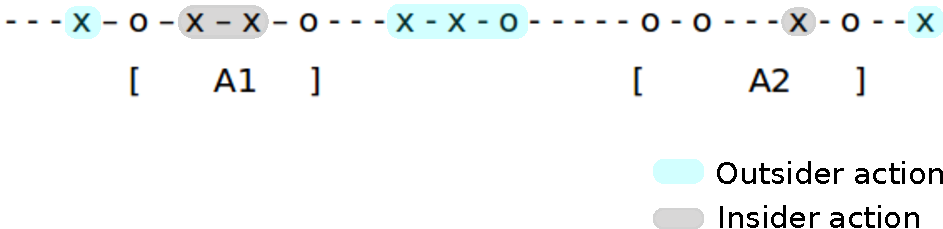
\includegraphics[width=\textwidth]{clustering_ex_complete.pdf}
    \caption{Output of $SA^3$ for a concrete sequence of actions, where outsider and insider actions are identified.}
    \label{fig-initial-clusters}
\end{figure}

Figure \ref{fig-initial-clusters} shows that $SA^3$ detects activities $A_1$ and $A_2$ in that sequence of actions. As stated in Section \ref{sec:clustering:sa3} only actions that are in the IAM of the detected activity can be really considered part of that activity, i.e. only circles that are inside activities $A_1$ and $A_2$ are labelled with corresponding activity labels. 

Given that action classification, two new definitions can be assumed:

\begin{defn}[Insider action]
\label{def-insider}
 Every action that is inside initial clusters provided by $SA^3$ but is not in their IAMs is considered an \textit{insider action} or \textit{insider}, in short.
\end{defn}

\begin{defn}[Outsider action]
\label{def-outsider}
 Every action out of initial clusters provided by $SA^3$ is an \textit{outsider action} or \textit{outsider}, in short.
\end{defn}

Due to single-user single-activity scenario constraint (constraint \ref{cons-single}), an insider may pertain to its wrapping activity or to none, i.e. it has been produced by noise or user erratic behaviour. There is no chance for an insider to pertain to an activity other than its wrapping activity because such an assumption would imply the existence of interleaved activities. The situation for outsiders is different since an outsider can pertain to its previous activity, next activity or to none. 

The inherent difference between insiders and outsiders demands a different treatment for both cases. $AC$ first treats all insider actions and afterwards computes all outsiders using different approaches.

\subsection{Insider actions}
To decide whether an insider has to be added to its wrapping activity, a \textit{compatibility function} between an activity and an action is defined. The compatibility function is a boolean function that captures whether an insider action has been executed in the same location as the activity and its purpose is coherent with the activity type:

\begin{equation}
\label{eq-comp}
 Comp(A, a) = Loc(A, a) \wedge Type(A, a)
\end{equation}

\noindent where $A$ is an activity and $a$ is an action. $Loc(A, a)$ is the location compatibility between an activity and an action, defined as in Section \ref{subsec:clustering:sa3:find}. The location of the concrete activity $A$ is inferred using the same process as in $SA^3$, i.e. the common location of the actions pertaining to the IAM of the activity is set to be the location of the activity. $Loc(A, a)$ returns whether the inferred location for action $a$ is the same as the inferred location for activity $A$. On the other hand, $Type(A, a)$ is the type compatibility between an activity and an action. Action type is inferred from the object used to execute the action. Every object in the context knowledge has a list of types. Activity type is unique and it is also retrieved from the context knowledge file. So $Type(A, a)$ is calculated as the intersection between the list of types of the action $a$ and the type of the activity $A$. If the intersection is empty, the action and the activity are not type compatible.

Hence an insider action $a$ will only be aggregated to its wrapping activity $A$, if $Comp(A, a) = True$, i.e. the insider has been executed in the same location of the activity, and its purpose is compatible with the activity type. If $Comp(A, a) = False$, the insider will be labelled with the None label, which means that it is not part of any activity.

\subsection{Outsider actions}
As an outsider can be aggregated to its previous or next activity, first of all the algorithm checks the feasibility of both options, defining another boolean function called \textit{candidate function}:

\begin{equation}
\label{eq-candidate}
 Cand(A, a) = Comp(A, a) \wedge InRange(A, a)
\end{equation}

\noindent $Comp(A, a)$ has already been defined in equation \ref{eq-comp}, so the candidate function also takes into account location and type. $InRange$ function is another boolean function that captures time feasibility. Thus the candidate function states that an activity $A$ is a candidate activity for action $a$, if they are compatible ($Comp(A, a) = True$) and in range ($InRange(A, a) = True$). 

As commented above, $InRange$ function has been defined to capture the time feasibility. For example, if an action has been executed two hours before an activity whose estimated duration is three minutes, the action should not be aggregated to that activity, since it is almost impossible for the action to be related with the activity. This reasoning can be implemented in a boolean function using time distance and activity duration.

To capture time feasibility, the duration given by the expert in an IAM is interpreted as the standard deviation for concrete executions of that activity, i.e. the vast majority of the activities executed by any user, will lie inside the time area limited by the duration. This can be seen in Figure \ref{fig-in-range}. So time distances among actions pertaining to a concrete activity are modelled by a Gaussian distribution, where the duration estimation given by the expert for that activity is the standard deviation. A Gaussian distribution has been selected, because it captures perfectly the idea of activity duration as a time estimation where the majority of executions of that activity occur. The probability for actions of an activity to lie in the area limited by the duration estimation is very high and gets lower as it gets further from that duration.

Nevertheless, due to human behaviour variations, there will be some executions whose duration is outside the standard deviation. To capture those executions, $InRange$ function considers all the actions lying inside $k$ standard deviations. For the experiments run in this dissertation $k=2$ has been set, but the value can be adjusted depending on the area which is desired to cover. For a concrete activity execution, the mean of the activity is calculated as the centre of the detected start and end of the activity, as given by $SA^3$. Using this mean calculation, duration estimation given in the context knowledge is the standard deviation of the Guassian distribution for action time distances. Hence, in the case depicted in Figure \ref{fig-in-range}, where Gaussian distributions are calculated as described, the outsider action represented with a star is in range with activities $A_1$ and $A_2$ for $k=2$.

\begin{figure}[!t]
\centering
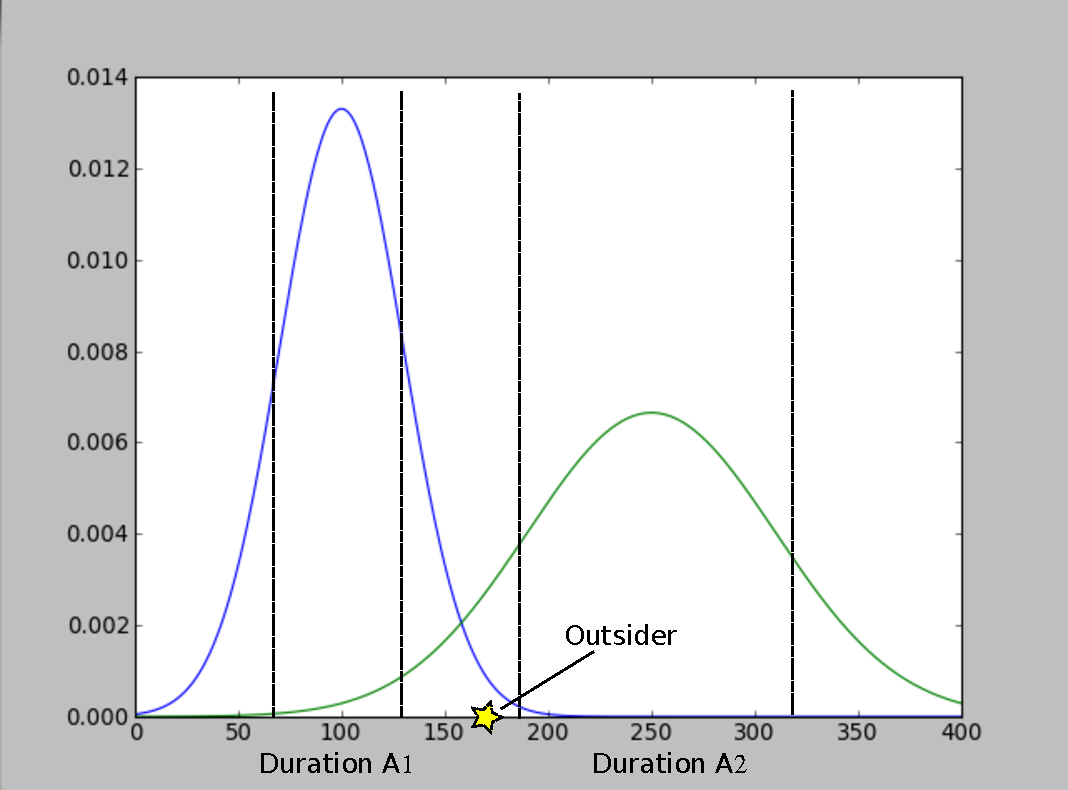
\includegraphics[width=\textwidth]{in_range_criterion.pdf}
    \caption{Gaussian distributions of activity durations for activities $A_1$ and $A_2$. Vertical lines show the standard deviation and the star represents an outsider action.}
    \label{fig-in-range}
\end{figure}

In consequence, using the candidate function, the following cases can be faced for an outsider action $a$ and surrounding activities $A_1$ and $A_2$:

\begin{enumerate}
 \item $Cand(A_1, a) = Cand(A_2, a) = False \rightarrow$ $a$ is noise (None label)
 \item $Cand(A_1, a) = True \wedge Cand(A_2, a) = False \rightarrow$ aggregate $a$ to $A_1$
 \item $Cand(A_1, a) = False \wedge Cand(A_2, a) = True \rightarrow$ aggregate $a$ to $A_2$
 \item $Cand(A_1, a) = Cand(A_2, a) = True \rightarrow$ need of a new heuristic
\end{enumerate}

The first three cases provide a clear classification for an outsider. The candidate function determines unambiguously the label for action $a$. But for the fourth case, where previous and next activities are both candidate activities, a new heuristic has to be defined. There is no more information in the context knowledge than the location and type information to relate outsider actions to activities, thus context knowledge cannot be used to decide between activities $A_1$ and $A_2$. Hence a new heuristic is defined stating that an outsider action $a$ will be aggregated to the time closest activity:

\begin{equation}
 min\{\Delta_t(A_1, a), \Delta_t(A_2, a)\}
\end{equation}

To implement this heuristic, a definition for $\Delta_t(A, a)$, the time distance between an activity and an action, is needed. As an activity has a duration and an action is described by a time instant, three time metrics are proposed:

\begin{enumerate}
 \item Simple time distance: the distance between the centre of the activity as given by $SA^3$ and the action time coordinate.
 \begin{equation}
 \label{eq-t1}
  \Delta_t(A, a) = | C_A - t_a |,\ where \ C_A = \frac{t_{end} ^{SA^3} - t_{start} ^{SA^3}}{2}
 \end{equation}
 \item Normalised time distance: simple time distance normalised by the duration of the activity as given by the expert. This time metric, as opposed to the simple time distance, treats equally all activities regardless their duration. Notice that duration given by the expert is used rather than the duration detected by $SA^3$, since $SA^3$ may give varying durations depending on the order of executed actions that pertain to the IAM of the detected activity. Hence, the duration given by $SA^3$ cannot be a good reference. But notice also that to calculate the centre of the activity, the output of $SA^3$ is used. In this case, this information is the only one that allows calculating the centre. So the duration given by the expert is projected symmetrically around the centre calculated from $SA^3$:
 \begin{equation}
 \label{eq-t2}
  \Delta_t(A, a) = \frac{| C_A - t_a |}{Duration_A} ,\ where \ C_A = \frac{t_{end} ^{SA^3} - t_{start} ^{SA^3}}{2}
 \end{equation}
 \item Dynamic centre normalised time distance: only used for previous activity, it dynamically calculates the centre of the activity depending on already aggregated actions.
 \begin{equation}
 \label{eq-t3}
  \Delta_t(A, a) = \frac{| C_A - t_a |}{Duration_A} ,\ where \ C_A = \frac{t_{start} ^{AC} + Duration_A}{2}
 \end{equation}
\end{enumerate}

Let us explain the third time distance in detail. Activity start and end times provided by $SA^3$ are not generally trustful, since they depend on what actions are in the IAM of the detected activity and on the order of executions of those actions by the user. Imagine that $IAM(A)=\{a, b\}$ and that the action sequence processed by $SA^3$ is $S=\{d, b, a, c\}$. Assume that sequence $S$ is the action sequence performed by the user for activity $A$. $SA^3$ will detect that activity $A$ is being performed in sequence $S$, but it will only label actions $b$ and $a$ as pertaining to the activity. $SA^3$ does not have any information to know whether actions $d$ and $c$ pertain to activity $A$. So the start time of activity $A$ for $SA^3$ will be the time-stamp associated to action $b$ and not to action $d$. The same happens for the activity end time.

Nevertheless, while executing the $AC$ algorithm, starting times of activities can be estimated better, but with some limitations. In the previous example, as outsiders in $AC$ are treated in time order for convenience, when treating outsider $c$, its previous activity's previous actions have already been treated (in this case, action $d$). $AC$ has already determined that action $d$ pertains to activity $A$. This means that the start of that previous activity $A$ has been fixed and it is different from the start time provided by $SA^3$ ($t_{start} ^{AC} \neq t_{start} ^{SA^3}$).

In contrast with time metrics 1 and 2, where activity start and end were given by $SA^3$ and activity duration was assumed to be located symmetrically around the centre of the activity, the third time metric uses the start time of the previous activity as found by $AC$. Afterwards, the centre of the activity is calculated projecting the duration from the starting point. This makes previous activity treatment more accurate. However, notice that the same approach cannot be applied to the next activity, since it has not been treated yet. The estimation given by $SA^3$ cannot be improved, because surrounding activities have not been treated when action $c$ is being analysed. Hence, the best guess is to keep using start and end times provided by $SA^3$.

\subsection{The complete AC algorithm}

To sum up, the $AC$ algorithm takes the results of $SA^3$ as the initialisation step. First, it treats insiders for all the activities detected by $SA^3$, using the compatibility function (equation \ref{eq-comp}). Afterwards, it treats outsiders in time order, using the candidate function (equation \ref{eq-candidate}) and defined three time metrics (equations \ref{eq-t1}, \ref{eq-t2} and \ref{eq-t3}). The complete algorithm is depicted as pseudo-code in Algorithm \ref{alg:ac}.

\begin{algorithm}
 \caption{$AC$ algorithm for activity clustering}
 \label{alg:ac}
 \begin{algorithmic}
 \REQUIRE partially\_annotated\_dataset, context\_knowledge
 \ENSURE fully\_annotated\_dataset, activity\_clusters
 \STATE $fully\_annotated\_dataset \leftarrow createDataset(partially\_annotated\_dataset)$
 \STATE $insiders \leftarrow obtainInsiders(partially\_annotated\_dataset)$
 \STATE $outsiders \leftarrow obtainOutsiders(partially\_annotated\_dataset)$ 
 \FORALL{$action \in insiders$}
  \STATE $activity \leftarrow obtainWrappingActivity(action, partially\_annotated\_dataset)$
  \IF{$Comp(activity, action, context\_knowledge)$}
    \STATE $label(a, activity, fully\_annotated\_dataset)$
  \ELSE
    \STATE $label(a, None, fully\_annotated\_dataset)$
  \ENDIF
 \ENDFOR 
 \FORALL{$action \in outsiders$}  
  \STATE $previous\_activity \leftarrow obtainPreviousActivity(action, partially\_annotated\_dataset)$
  \STATE $next\_activity \leftarrow obtainNextActivity(action, partially\_annotated\_dataset)$
  \STATE $Prev \leftarrow Cand(action, previous\_activity, context\_knowledge)$
  \STATE $Next \leftarrow Cand(action, next\_activity, context\_knowledge)$
  \IF{$\neg Prev \wedge \neg Next$}
    \STATE $label(a, None, fully\_annotated\_dataset)$
  \ELSIF{$Prev \wedge \neg Next$}
    \STATE $label(a, previous\_activity, fully\_annotated\_dataset)$
  \ELSIF{$\neg Prev \wedge Next$}
    \STATE $label(a, next\_activity, fully\_annotated\_dataset)$
  \ELSIF{$Prev \wedge Next$}
    \STATE $// \text{Use time metrics}$
    \STATE $prev\_dist \leftarrow timeDist(action, previous\_activity, time\_metric)$
    \STATE $next\_dist \leftarrow timeDist(action, next\_activity, time\_metric)$
    \IF{$prev\_dist \leq next\_dist$}
      \STATE $label(a, previous\_activity, fully\_annotated\_dataset)$
    \ELSE
      \STATE $label(a, next\_activity, fully\_annotated\_dataset)$
    \ENDIF
  \ENDIF  
 \ENDFOR
 \STATE $activity\_clusters \leftarrow createClusters(fully\_annotated\_dataset)$
 \RETURN $fully\_annotated\_dataset, activity\_clusters$
 \end{algorithmic}
\end{algorithm}

The algorithm returns two files: (i) a fully labelled sensor activation dataset, which is formatted in a CSV file in the current implementation, and (ii) a list of clusters, which has been implemented through a \textit{Json} file. Additionally, that file contains: (i) the frequency of each activity cluster, (ii) duration statistics (mean and standard deviation), (ii) frequencies of used objects and actions and (iii) frequencies of locations per activity. 

An example of the fully annotated dataset can be seen in Figure \ref{fig-fully-annotated}. $AC$ takes the partially annotated dataset generated by $SA^3$ and adds two new columns: the label assigned by $AC$ and the start and end tags for activities. Figure \ref{fig-fully-annotated} is taken from a real experiment and shows very well the difference between $SA^3$ and $AC$. The action sequence depicted shows a particular execution of the MakePasta activity, where due to sensor errors, a \textit{rcontrolSens} activation occurred. It can be seen how $SA^3$ detects that a MakePasta activity is being performed in the action sequence. But activity start and end times differ substantially from the real ones. However, $AC$ detects perfectly activity start and end times, using the outsider action treatment process. And for the insider action \textit{hasRemoteControl}, $AC$ assigns a None label, since the action is not type compatible with the activity. So in this case, $AC$ completes its work perfectly, assigning the appropriate labels to every action and enhancing the results obtained by $SA^3$.

\begin{figure}[htbp]
\begin{scriptsize}
\begin{lstlisting}
2014-05-23 13:34:09.590934,storeSens,openStore,None,,MakePasta,start
2014-05-23 13:34:15.976283,potSens,useCookingUtensil,MakePasta,start,MakePasta,
2014-05-23 13:34:35.067066,ktapSens,turnOnTap,MakePasta,,MakePasta,
2014-05-23 13:35:01.608632,cookerSens,useCookingAppliance,MakePasta,,MakePasta,
2014-05-23 13:35:59.858079,rcontrolSens,hasRemoteControl,MakePasta,,None,
2014-05-23 13:36:15.475288,macaroniSens,hasPasta,MakePasta,end,MakePasta,
2014-05-23 13:45:15.485760,drainerSens,useCookingUtensil,None,,MakePasta,
2014-05-23 13:45:54.969772,fridgeSens,openFridge,None,,MakePasta,
2014-05-23 13:46:00.132993,baconSens,hasBacon,None,,MakePasta,
2014-05-23 13:46:05.764809,creamSens,hasCream,None,,MakePasta,end
\end{lstlisting}
\end{scriptsize}
\caption{Example of a fully annotated dataset, one of the outputs of the $AC$ algorithm.}
\label{fig-fully-annotated}
\end{figure}

An example of the activity clusters file has already been shown in Figure \ref{fig-clusters-file}. As it can be seen in the figure, several concepts per activity are stored in the file:

\begin{enumerate}
 \item Locations: a list of different locations where the activity has been performed with occurrence frequencies. Locations are obtained using activity location inference.
 \item Actions: a list of actions executed by the user to perform the activity with associated occurrence frequencies.
 \item Patterns: patterns refers to different action sequences performed by the user for the activity, i.e. the activity clusters detected by the clustering process. Every detected cluster has its occurrence frequency. 
 \item Objects: a list of objects used by the user while performing the activity. Once again, every object has its occurrence frequency.
 \item Occurrences: the total number of instances of the activity captured by the clustering process, which has to be equal to the sum of all the occurrences of patterns. 
 \item Duration: the mean duration of the detected instances of the activity and the standard deviation, both in seconds.
\end{enumerate}

This information will be used by the Activity Model Learner ($AML$) algorithm to learn EAMs from the clusters extracted by the clustering process. Additionally, the information stored in the activity clusters file may be very useful to domain experts, since they may be able to analyse how activities are carried out by different users in terms of the executed actions, used objects, different sequences of actions and duration. The potential applications of such information, specially considering that it can be updated periodically to monitor the evolution of the user, is out of the scope of this dissertation, but it can open the doors to detect cognitive impairment and its evolution, inappropriate behaviour or user bad habits. 
\section{Summary and Conclusions}
\label{sec:clustering:sum}

A two-step clustering process has been developed and implemented in this chapter, in order to detect and identify activities in a sensor activation dataset using the context knowledge provided by a domain expert. The first step of the clustering process has been devoted to find the occurrences of IAMs in an unlabelled sensor activation dataset. For that purpose, a novel pattern recognition algorithm has been developed, which uses IAMs as patterns, but also takes into account duration, location and completeness criteria. The algorithm is called $SA^3$ and it can work in scenarios where actions can appear in varied orders and positive and missing sensor noise exist.

The initial clusters detected by $SA^3$ are then expanded in the second step of the clustering process. The $AA$ algorithm distinguishes between insider and outsider actions. For the former group of actions, a compatibility function has been defined to decide whether an insider belongs to its wrapping activity, whereas for the latter group, previous and next activities are analysed in terms of compatibility and time feasibility. For those actions which can be aggregated to the previous and the next activities, three time metrics have been defined. Using those metrics, the actions are aggregated to the time closest activity. 

The results of the clustering process are finally stored in two files: the fully annotated dataset, where every sensor activation has an activity label, and the activity clusters file, where different clusters for each activity are depicted alongside other information. Even though the clustering process has to be understood inside the global solution designed to learn extended activity models, it can also be used for further objectives. For instance, it can be used to annotate sensor activation datasets. Notice that manual methods are usually used for annotating datasets that are used for activity recognition applications. However, manual annotation has a lot of problems, namely it is prone to errors and it is very time consuming, as shown by Rashidi and Cook in \cite{Rashidi2011}. Hence, the developed activity clustering process for unlabelled sensor activation datasets can be used as an activity annotator method, as far as required previous knowledge can be provided. 


%: ----------------------- activity model learner ------------------------

% this file is called up by thesis.tex
% content in this file will be fed into the main document

%: ----------------------- introduction file header -----------------------
\begin{savequote}[50mm]
If I have seen further it is by standing on the shoulders of giants.
\qauthor{Isaac Newton}
\end{savequote}

\chapter{Related Work}
\label{cha:soa}

% the code below specifies where the figures are stored
\ifpdf
    \graphicspath{{2_state_of_the_art/figures/PDF/}{2_state_of_the_art/figures/PNG/}{2_state_of_the_art/figures/}}
\else
    \graphicspath{{2_state_of_the_art/figures/EPS/}{2_state_of_the_art/figures/}}
\fi

%\letra{D}{escribe} how the state of the art has been structured in this chapter, referencing sections and commenting on their contents. Justify the topics covered by the chapter.

\letra{H}{uman} activity recognition is a broad research area which can be analysed from many different points of view. The objective of this chapter is to provide a high-level picture of the current status of the research topic, to then describe more in detail the concrete approaches that are related to the work presented in this dissertation. 

First of all, Section \ref{sec:soa:har} introduces the concept of \textit{Human Activity Recognition}, shows its main applications and provides a high-level taxonomy of activity recognition approaches. Section \ref{sec:soa:sensor} describes in detail the category in which this dissertation fits regarding the monitoring approach: \textit{Sensor-Based Activity Recognition}. Based on the specific sensors used for activity monitoring, Section \ref{sec:soa:monitoring} presents a more detailed taxonomy for the category of sensor-based activity recognition. On the other hand, the following sections analyse the main currents of activity modelling, which is the focus of this dissertation: Section \ref{sec:soa:datadriven} presents \textit{Data-Driven Approaches}, while Section \ref{sec:soa:knowledgedriven} describes in detail \textit{Knowledge-Driven Approaches}. A summary and comparison of both activity modelling currents is provided in Table \ref{tab:soa:comparison}. Some recent work has settled the basis to combine both currents, giving as result the \textit{Hybrid approaches}, as shown in Section \ref{sec:soa:hybrid}. This dissertation is another step in order to achieve hybrid approaches that can combine effectively the best features of knowledge- and data-driven approaches. The chapter finalises with Section \ref{sec:soa:summary}, where a concise summary is provided alongside with some conclusions.
\section{The Learning Algorithm}
\label{sec:learner:algorithm}

Activity clusters extracted by the clustering process contain all the action sequences performed by a user for each activity. But some of those clusters are spurious, due to sensor noise, user erratic behavior and clustering errors. The objective of $AML$ is to remove spurious action sequences. For that purpose, a three-step algorithm has been designed and implemented. For all the clusters extracted for an activity, the following steps are performed:

\begin{enumerate}
 \item Remove repeated actions into a sequence: some action sequences contain repeated actions. For instance, consider the sequence $S=\{a, b, a, c\}$. As repeated actions do not add any new information for activity modeling, they are removed. $S$ becomes $S' = \{a, b, c\}$. Notice that this step does not remove any action sequence of an activity.
 \item Fuse equal action sequences: some action sequences contain the same actions, but in different orders. For example, $S_1 = \{a, b, c \}$ and $S_2 = \{b, c, a\}$. The order of actions is not important for activity models, so both sequences are fused. To detect equal sequences, the Jaccard coefficient is used \cite{A.K.Jain1988}. The Jaccard coefficient between two sequences $A$ and $B$ is defined as:
 \begin{equation}
  Jaccard(A, B) = \frac{A \cap B}{A \cup B}
 \end{equation}
Any two sequences whose Jaccard coefficient is 1 are fused. Fusing means removing one of the sequences and adding frequencies to store in the remaining sequence.
 \item Run Jaccard based outlier detection algorithm, which has been specially designed to learn proper action sequences.
\end{enumerate}

The Jaccard based outlier detection is an iterative algorithm. It calculates the so called \textit{Jaccard Matrix} ($JM$), which is a square matrix of remaining action sequences. $JM_{i, j}$ stores the Jaccard coefficient for action sequences $i$ and $j$. The diagonal of $JM$ is 1, since two equal action sequences' Jaccard coefficient is 1. Removing diagonal values $\hat{JM}$ is obtained, which is used to calculate the median and the standard deviation to the median. The median is used rather than the mean value, since the median is robust to outliers. Using those statistics a threshold $\theta$ is calculated, such that:

\begin{equation}
 \theta = max \{ median(\hat{JM}) + std(\hat{JM}), \lambda \}
\end{equation}

The first part of the calculation of $\theta$ captures the relative similarity among all action sequences and establishes an adequate threshold to identify outliers. However, as the Jaccard coefficient is defined in an absolute scale, the second part ($\lambda \in [0, 1]$) has to be added. For relatively short action sequences used in the experiments (the longest ones are around 9 actions), 0.75 has shown to be a good balanced value. $\lambda$ prevents fusing sequences that even being more similar than most of the others, their similarity is not higher than it. Sequences below $\lambda$ are considered too different to be fused. 

The algorithm fuses sequences whose Jaccard coefficient is higher than $\theta$, until no sequences can be fused. To fuse, the sequence with lowest frequency is removed and its frequency value is added to the frequency of the other sequence. This fusing heuristic states that the lower frequency sequence is a spurious variation of the higher frequency sequence. 


%: ----------------------- Evaluation ------------------------


% this file is called up by thesis.tex
% content in this file will be fed into the main document

%: ----------------------- introduction file header -----------------------
\begin{savequote}[50mm]
If I have seen further it is by standing on the shoulders of giants.
\qauthor{Isaac Newton}
\end{savequote}

\chapter{Related Work}
\label{cha:soa}

% the code below specifies where the figures are stored
\ifpdf
    \graphicspath{{2_state_of_the_art/figures/PDF/}{2_state_of_the_art/figures/PNG/}{2_state_of_the_art/figures/}}
\else
    \graphicspath{{2_state_of_the_art/figures/EPS/}{2_state_of_the_art/figures/}}
\fi

%\letra{D}{escribe} how the state of the art has been structured in this chapter, referencing sections and commenting on their contents. Justify the topics covered by the chapter.

\letra{H}{uman} activity recognition is a broad research area which can be analysed from many different points of view. The objective of this chapter is to provide a high-level picture of the current status of the research topic, to then describe more in detail the concrete approaches that are related to the work presented in this dissertation. 

First of all, Section \ref{sec:soa:har} introduces the concept of \textit{Human Activity Recognition}, shows its main applications and provides a high-level taxonomy of activity recognition approaches. Section \ref{sec:soa:sensor} describes in detail the category in which this dissertation fits regarding the monitoring approach: \textit{Sensor-Based Activity Recognition}. Based on the specific sensors used for activity monitoring, Section \ref{sec:soa:monitoring} presents a more detailed taxonomy for the category of sensor-based activity recognition. On the other hand, the following sections analyse the main currents of activity modelling, which is the focus of this dissertation: Section \ref{sec:soa:datadriven} presents \textit{Data-Driven Approaches}, while Section \ref{sec:soa:knowledgedriven} describes in detail \textit{Knowledge-Driven Approaches}. A summary and comparison of both activity modelling currents is provided in Table \ref{tab:soa:comparison}. Some recent work has settled the basis to combine both currents, giving as result the \textit{Hybrid approaches}, as shown in Section \ref{sec:soa:hybrid}. This dissertation is another step in order to achieve hybrid approaches that can combine effectively the best features of knowledge- and data-driven approaches. The chapter finalises with Section \ref{sec:soa:summary}, where a concise summary is provided alongside with some conclusions.
\section{Evaluation Methodology}
\label{sec:evaluation:methodology}

% Talk about standard evaluation methodology and its drawbacks
Even though activity recognition is very diverse in terms of sensor approaches and algorithmic choices, evaluation is usually carried out applying a very well known methodology \cite{Riboni2011a} \cite{Rashidi2011} \cite{Tapia2004} which can be summarised in the following steps:

\begin{enumerate}
 \item Choose a target environment and deploy sensors to acquire and process information about human activities. 
 \item Select a group of people who can perform target activities in the prepared environment.
 \item Select a dataset labelling system so datasets generated by users can be used as a ground truth, both for the activity recognition system and the evaluation process.
 \item Run experiments with users and label the obtained activity datasets.
 \item Use the same datasets to test the activity recognition system and store the labels produced by it.
 \item Compare the labels of the activity recognition system with the ground truth using appropriate metrics.
\end{enumerate}

% Insert a diagram that shows the standard methodology

Each of the enumerated steps may vary depending on the activity recognition approach and the available resources. The described methodology, which will be called \textit{standard methodology} for the rest of the dissertation, is conventionally the reference for any group working on human activity recognition.

Nevertheless, there are some problems that make very difficult to implement the so called standard methodology. For instance, (i) it is not always possible to own an environment and install sensors and processing systems, due to economic reasons, (ii) running experiments with human beings imply ethical and legal issues that can slow down the research process or sometimes make it impossible, (iii) dataset labelling systems are not perfect, since most of them rely on users' memory or discipline to annotate every activity carried out, and (iv) regulatory limitations on the use of human subjects prohibit the collection of extensive datasets that can test all scenarios and theories under all circumstances. 

There are several research groups who have made publicly available the datasets that they obtain in their pervasive environments, following different variants of the standard methodology. A Wiki Page called BoxLab\footnote{http://boxlab.wikispaces.com/List+of+Home+Datasets} contains a detailed list of public datasets collected in home environments. It contains a description of the deployed sensors, whether it is an annotated dataset and the availability of the dataset. Those public datasets can be a very good alternative for those research groups which cannot run their own experiments. Furthermore, public datasets can also be used for benchmarking different activity recognition systems.

%This paper presents a novel evaluation methodology to overcome the enumerated problems. The methodology has been named \textit{hybrid} because it combines real users' inputs and simulation tools. The key idea is to circulate surveys among target users with the objective of capturing how they perform certain activities of daily living. Using the information collected by surveys, individual scripts are prepared, which are then processed by a synthetic dataset generator tool to simulate arbitrary number of days and generate perfectly labelled datasets of activities. To get as close as possible to real world settings, the synthetic dataset generator uses probabilistic sensor noise models and probabilistic time lapses.

% Present the hybrid methodology and show its need and benefits

\subsection{Analysis of the viability of the standard methodology for the extended activity model learning system}

To evaluate properly the EAM learning system, activity datasets that fulfil several conditions are needed. Namely:

\begin{enumerate}
 \item Contain a lot of samples of different activities to enable a proper learning process. To make data-driven learning a meaningful process, many samples of the same activities are needed, specially to learn noise free activity models. If few samples are available and those samples are affected by noise, it is very difficult for the learning process to distinguish between noisy and noiseless models.
 \item Sensor activations must be labelled in order to provide a solid ground truth. An accurate evaluation process needs an accurately labelled dataset, where all sensor activations produced due to an activity execution are annotated with that activity name, whereas sensor noise is not included in the activity.
 \item Specific objects used for activities have to be monitored (dense sensing scenario). Instead of getting data from context sensors such as thermometers, humidity sensors or even movement sensors, datasets have to contain sensor activations monitoring concrete objects such as cups, dishes, food and so on, in order to be able to produce accurate activity models.
 \item At least some of the activities have to be performed in varied ways to see whether the presented learning process can capture all those variations. Different ways of performing the same activity are needed, since the EAM learning system aims at capturing sub-activities. If all the activities are performed the same way in terms of executed actions, the dataset will only serve to evaluate the learning of complete models, but not specialised models.
 \item Several users are needed as the approach aims at capturing personalised activity models for concrete users. Every user has his/her own way to perform the same activities and one of the objectives of the EAM learning system is to be able to model those personalised models. Thus, to show that the EAM learning system can really deal with different users, datasets of several users are required.
\end{enumerate}

Following the standard methodology to generate such datasets implies a high-cost and lengthy process with many ethical and legal constraints regarding the use of people for experiments. That cost, both economical and time cost, could not be assumed during the development of the current dissertation. Due to this limitation, public dataset repositories were analysed carefully to find an appropriate dataset.

Unfortunately, datasets that meet all the enumerated conditions could not be found in those public repositories. Some datasets used different activity monitoring approaches, such as vision- and wearable-based monitoring. Some other datasets could be used for the dense sensing scenario since they monitor specific objects, but activities are performed from a list where no variations can be found. Yet other datasets are more focused on monitoring the contextual information, rather than concrete user-object interactions.

As Helal et al. state in their paper \cite{Helal2011}:

\blockquote{\textit{Access to meaningful collections of sensory data is one of the major impediments in human activity recognition research. Researchers often need data to evaluate the viability of their models and algorithms. But useful sensory data from real world deployments of pervasive spaces are very scarce. This is due to the significant cost and elaborate groundwork needed to create actual spaces. Additionally, human subjects are not easy to find and recruit. Even in real deployments, human subjects cannot be used extensively to test all scenarios and verify multitudes of theories. Rather, human subjects are used to validate the most basic aspects of the pervasive space and its applications, leaving many questions unanswered and theories unverified.}}

This is the case of the presented approach for EAM learning. It turns out that no datasets were found from real pervasive environments to verify the exposed theory. However, Helal et al. propose a solution to this problem in the same paper \cite{Helal2011}:

\blockquote{\textit{It is thus necessary to develop alternative and practical approaches to studying human activity recognition. Powerful and realistic simulation tools could be used to support the growing demand for test data. Simulations enable researchers to create focused synthetic replications of important events and activities under study. It can be easily changed and refined allowing researchers efficiently to experiment, analyze and fine-tune their models and associated algorithms. Simulation also allows a wider community of researchers to engage and collaborate to solve a specific problem. Hence, a design based on preliminary simulation studies would most likely to be a more robust and inclusive design. Also, a simulation model that mimics an existing real world pervasive space is most likely to answer more questions (and generate much more data) than the target actual space.}}

Following those ideas, simulation tools have already been used for activity recognition. For example,   Okeyo et al. use a synthetic data generator tool to simulate time intervals between sensor activations \cite{Okeyo2012a}. Their research is focused on sensor data stream segmentation, so the tool generates varying patterns of sensor activations in order to verify their approach. Liao et al. combine simulation tools and real data for activity recognition in \cite{Liao2006}. A more elaborated simulator has been developed by Bruneau et al. in \cite{Bruneau2009}: DiaSim. The DiaSim simulator executes pervasive computing applications by creating an emulation layer and developing simulation logic using a programming framework. However, it is more focused on simulating applications such as fire situations, intrusions, etc. to identify potential conflicts. In consequence, DiaSim cannot be directly applied to activity recognition. Finally, Helal et al. propose to develop powerful and realistic simulation tools to study human activity recognition. They develop a simulator called \textit{Persim}, which has been enhanced in the new version \textit{Persim-3D} \cite{Helal2012}. Persim is an event driven simulator of human activities in pervasive spaces. Persim is capable of capturing elements of space, sensors, behaviours (activities), and their inter-relationships. Persim is becoming a very complete simulator tool for activity recognition in pervasive environments. However, it is still under development and one of the main limitations is that it does not provide a way to model realistically human behaviour. Authors have already identified this limitation and they are currently working on programming by demonstration approaches to overcome the problem.

As can be seen in the literature review done in the paragraph above, simulation tools can be used for activity recognition, since they provide accurate enough datasets to verify some theories. However, none of the references given above specify a concrete methodology to use simulators to evaluate activity recognition approaches. There is no information about how activities should be defined, how different users can be modelled, sensor error models and so forth, which are key issues when using a simulator. Therefore, there is a lack of a sound methodology that addresses the usage of simulation tools for activity recognition evaluation. 

\subsection{Hybrid evaluation methodology approach}
\label{subsec:evaluation:hybrid}

\begin{comment}
 - Describe target scenario: dense sensing, single user - single activity
 - Explain in detail the steps: survey, script writing, sensor modelling, synthetic dataset generator 
\end{comment}

The hybrid evaluation methodology has been specially designed for activity recognition systems which assume the dense sensing paradigm (see constraint \ref{cons-dense}). Even though the methodology itself is not limited to concrete scenarios, the implementation presented in this document works for single user - single activity scenarios, i.e. only one user is considered and concurrent or interleaved activities are not taken into account (see constraint \ref{cons-single}). 

The methodology has been named hybrid because it combines real users’ inputs and simulation tools. The key idea is to circulate surveys among target users with the objective of capturing how they perform certain activities of daily living. Additionally, users are also requested to describe how their days are in terms of defined activities. For example, a user might make a coffee and brush teeth in week days between 7:00 and 7:30 AM. So the aim of those surveys is to model real human behaviour, covering one of the major weaknesses of simulation-based evaluation methodologies. Using the information collected by surveys, individual scripts are prepared, which are then processed by a synthetic dataset generator tool to simulate arbitrary number of days and generate perfectly labelled datasets of activities. To get as close as possible to real world settings, the synthetic dataset generator uses probabilistic sensor noise models and probabilistic time lapses.

Based on those constraints and ideas, the proposed hybrid evaluation methodology has the following steps (see Figure \ref{fig-methodology}):

\begin{enumerate}
 \item Design activity surveys: to capture how users perform activities and model their behaviour, a proper survey has to be designed. A detailed explanation of how surveys are designed for this dissertation can be found in Section \ref{subsubsec:evaluation:survey}.
 \item Select target users: depending on the objectives of the research, several user groups can be selected. For example, if the system aims at providing help to elderly people, selecting members of that target group is recommended.
 \item Distribute surveys among target users: a suitable way to distribute surveys has to be used, which guarantees users' anonymity. The distribution method can also be influenced by target users. For example, using web-based surveys can be a bad idea if surveys are directed to elderly people, who can be unfamiliar with those technologies. Personal interviews may be a good alternative for those cases.
 \item Translate surveys to scripts: appropriate criteria have to be adopted to translate the answers obtained from surveys to scripts for the synthetic dataset generator - or any other simulator -. It is very important not to alter or lose the information provided by users.
 \item Model sensor noise: sensor noise has to be modelled in order to achieve realistic activity datasets. Real sensors are not perfect and depending on their technological base, error models have to be provided.
 \item Run synthetic dataset generator: using the scripts obtained from surveys and sensor error models, the synthetic dataset generator is executed. The output of the tool is a labelled activity dataset which will serve as the ground truth for evaluation.
 \item Develop the activity modelling and/or recognition system: researchers have to develop the activity modelling and/or recognition system in order to be tested. Notice that datasets generated by the synthetic dataset generator can also be used in this step, specially for data-driven approaches.
 \item Compare results: finally, the results obtained by the activity modelling and/or recognition system have to be compared with the ground truth, using appropriate metrics.
\end{enumerate}

\begin{figure}[htbp]
\centering
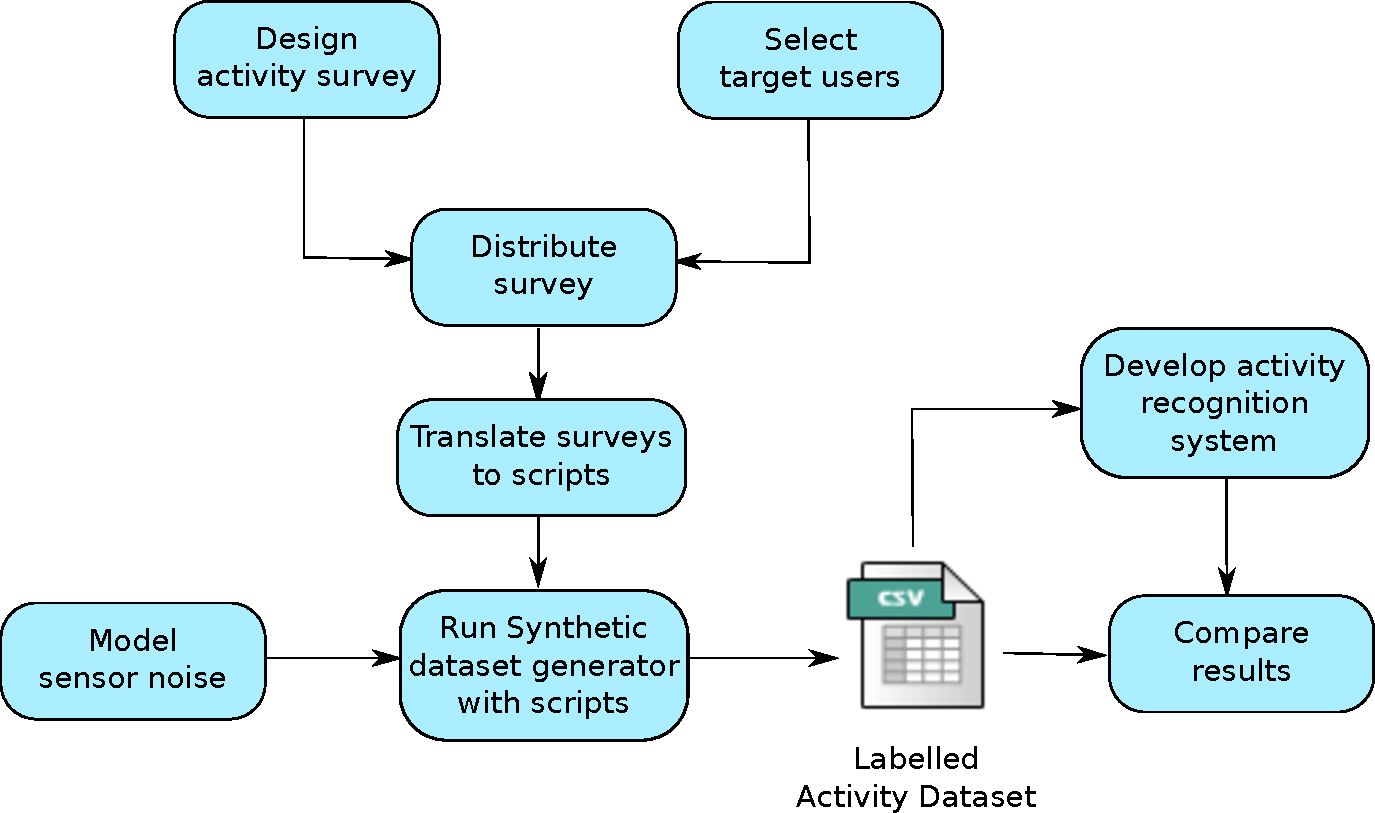
\includegraphics[width=12cm]{hybrid_methodology.pdf}
    \caption{The hybrid evaluation methodology steps depicted in a flowchart.}
    \label{fig-methodology}
\end{figure}

\subsubsection{Survey for activities of daily living}
\label{subsubsec:evaluation:survey}
\begin{comment}
 - Explain each of the questions of the survey
 - Show a screenshot and provide the link to the Google Form
 - Google Forms guarantee users' anonymity
 - Explain survey-script translation criteria
\end{comment}

One of the main advantages of considering dense sensing scenarios is that activities are described in terms of the objects which have been used to perform that activity. Furthermore, as only sensor activations (and not de-activations) are important for the approach (see definition \ref{def-sa}), to model an activity, it is enough to know which objects are used by the user and the order of usage of those objects. This information is easy to obtain in a survey and will be named \textbf{activity model}.

\begin{defn}[Activity model]
\label{def-act-model}
 An activity model is a sequence of objects used by a user to perform an activity. A user might provide several activity models per each defined activity, because the same activity can be performed in several ways. Activity models also provide a typical duration given by the user.
\end{defn}

On the other hand, to model human behaviour appropriately, acquiring activity models is not enough. It is very important to know what activities are performed by a concrete user in a daily basis, alongside with the time slots and time lapses between contiguous activities. 

\begin{defn}[Behaviour model]
\label{def-behaviour}
 A behaviour model is a sequence of activities with associated time slots and time lapses. A user might provide several behaviour models, as every day can be different in terms of performed activities and times.
\end{defn}

The main objective of the survey is to obtain activity and behaviour models from target users. Hence, the survey for activities of daily living has two main parts. The first part is devoted to capture what activities are performed in different days, i.e. behaviour models. The second part, on the other hand, asks users about how they perform those activities based on user-object interactions, i.e. activity models. The concrete survey used for the experiments carried out in this dissertation can be found in the web\footnote{http://goo.gl/etCNyi}. 

As can be seen in Figure \ref{fig-survey-1}, the survey begins with a brief explanation for target users, where the aims of the survey are stated and the target activities are presented. In this case, target activities are seven: make a coffee, make a chocolate, make pasta, brush teeth, watch television, wash hands and read a book. Afterwards, under the heading of ``Day Description'', users are asked to describe their week days in terms of activities. They are expected to provide information about time slots and activity sequences performed in those time slots. Users are also asked to provide time relations between two consecutive activities. For example, between 7:00 and 7:30 AM a user might make a coffee and ten minutes later might brush teeth. This first part has been designed to obtain behaviour models for target users.

\begin{figure}[htbp]
\centering
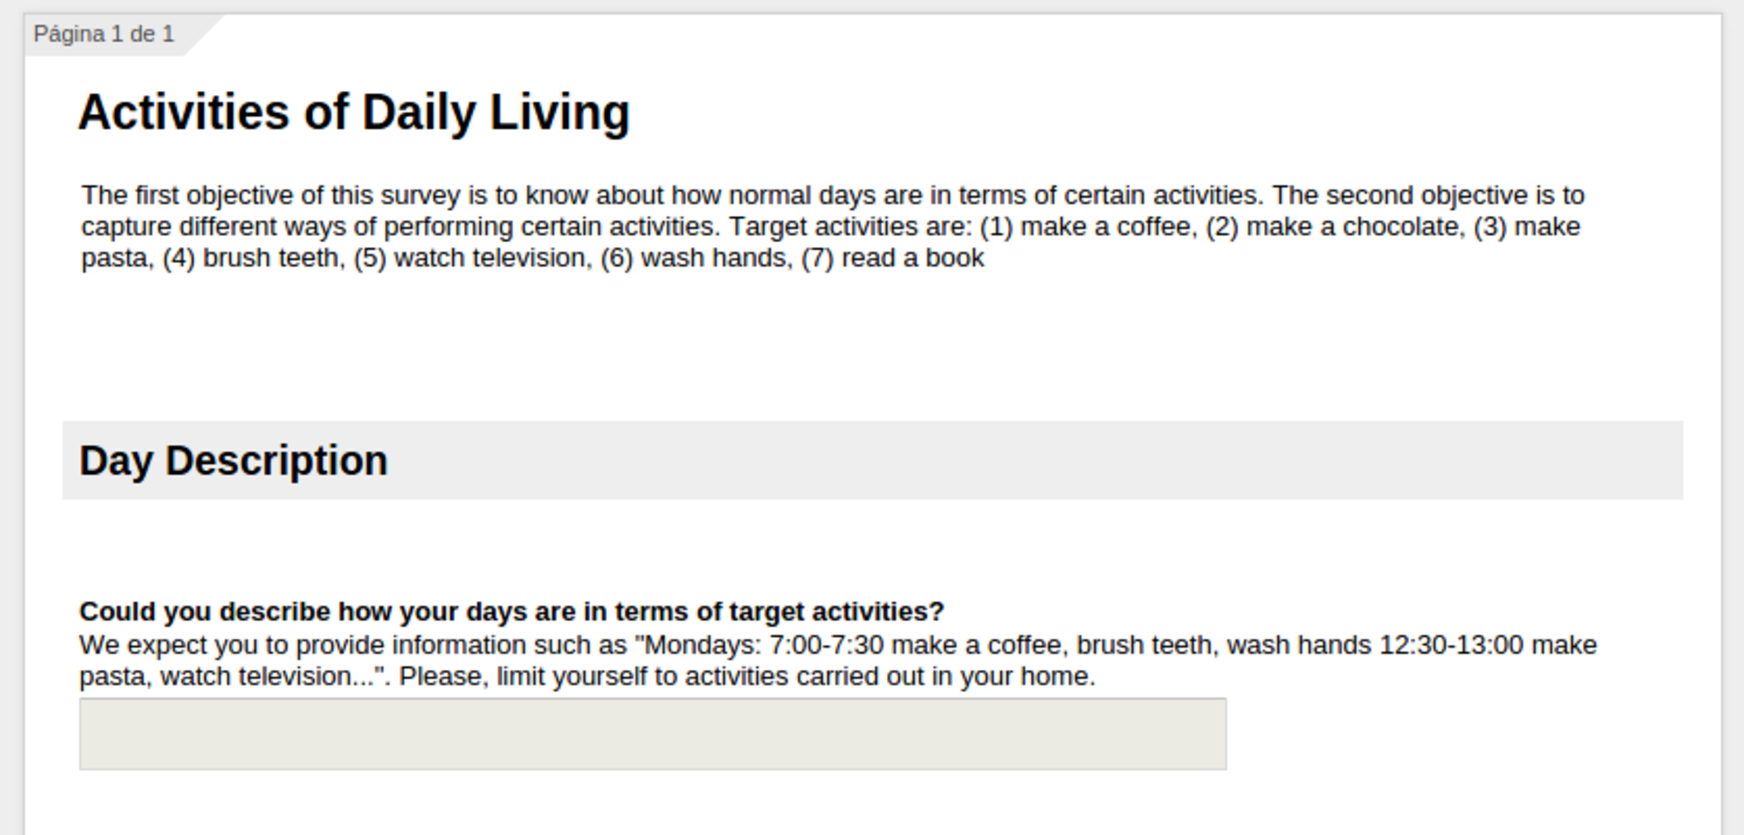
\includegraphics[width=\textwidth]{adl_survey_part1.pdf}
    \caption{The first part of the survey. A brief introduction can be found where the aim of the survey is explained, continuing with the behaviour model part.}
    \label{fig-survey-1}
\end{figure}

The second part of the survey is longer. Target activities are presented one by one. For each activity, several questions are asked to users, to capture the locations of activities, the ways activities are performed, the objects used for each activity, a description of how those objects are used and typical duration estimations. An example of those questions can be found in Figure \ref{fig-survey-2} for the activity MakeCoffee.

\begin{figure}[htbp]
\centering
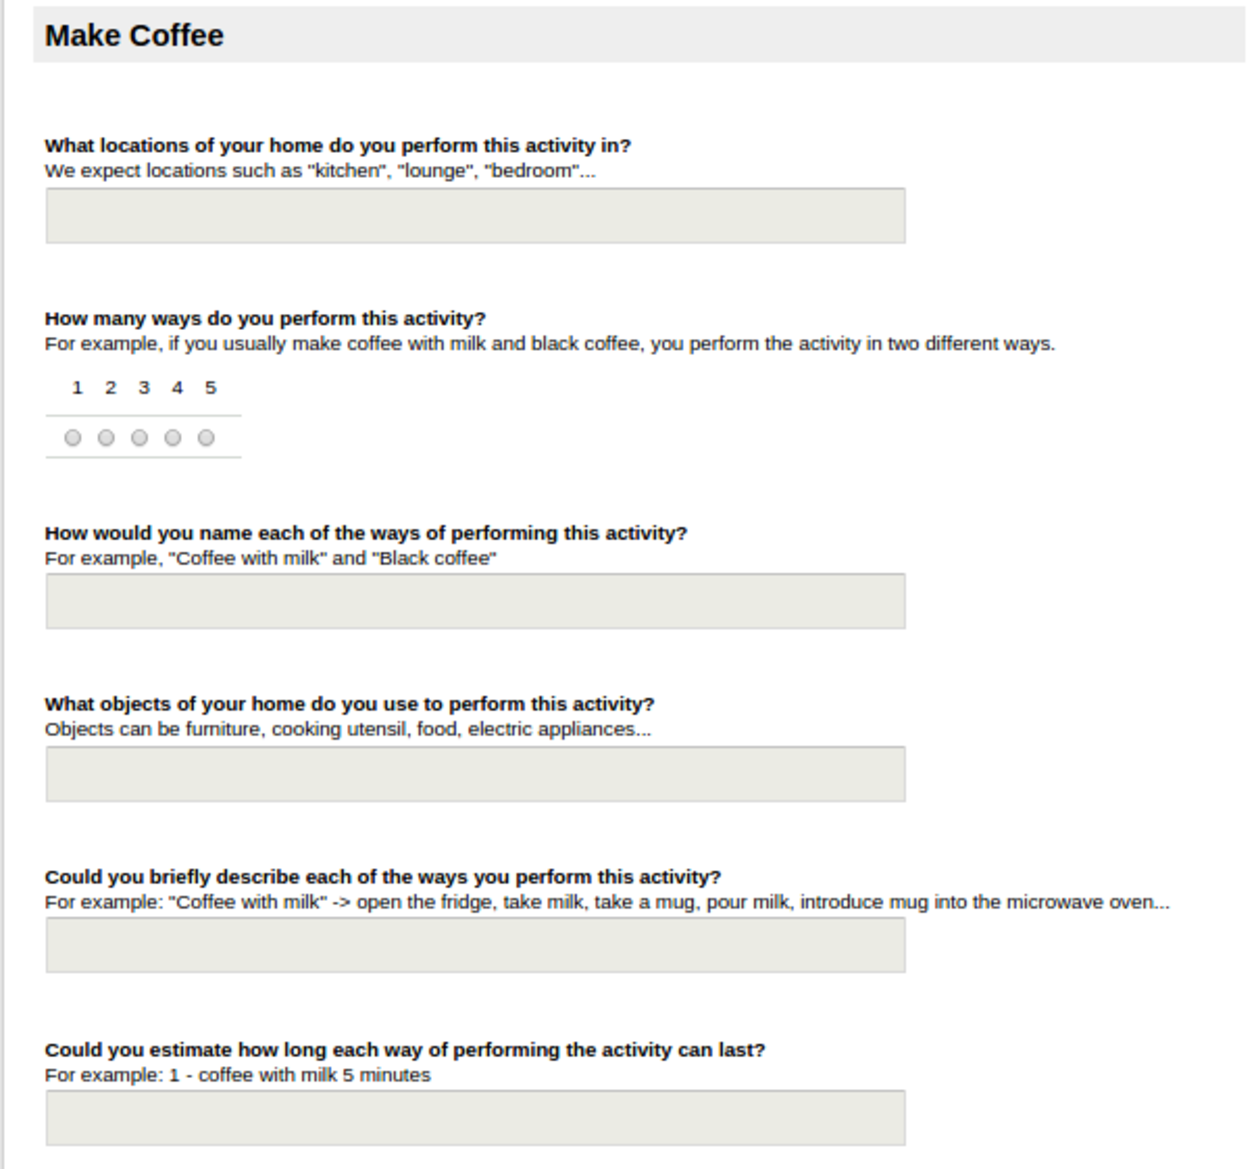
\includegraphics[width=\textwidth]{adl_survey_part2.pdf}
    \caption{The questions of the survey to capture the activity model of MakeCoffee.}
    \label{fig-survey-2}
\end{figure}

As Figure \ref{fig-survey-2} shows six questions are asked per activity. The first question is to know where the activity is performed by the user. As stated in the brief explanation under the question, expected locations are home locations such as kitchen, lounge, etc. Each activity may be performed in several locations, in concordance with the context knowledge model shown in Figure \ref{fig-context-json}. Notice also that the expected locations fulfil with the location definition given in definition \ref{def-location}.

The second question deals with different ways of performing an activity, i.e. sub-activities. Users are asked to provide a variation name, which will define the name of the sub-activity. The next question asks about the objects used to perform the activity. This will serve not only to model the activity itself, but also to model the context knowledge, where objects and attached sensors are represented (see Section \ref{subsec:approach:inputs}). Afterwards, the most important question for activity modelling comes: a description of how the enumerated objects are used to perform the activity. Descriptions are requested for each activity variation. From those descriptions, object usage order and time lapses will be obtained. Finally, the last question aims at modelling typical durations for the variations of the target activity.

As described in the steps of the hybrid evaluation methodology in Section \ref{subsec:evaluation:hybrid}, it is also important to decide the way to circulate the survey and to guarantee user anonymity. In our current experiments, we use the Google Forms\footnote{http://www.google.com/google-d-s/createforms.html} service, mainly for three reasons:

\begin{enumerate}
 \item Easy circulation: surveys can be sent by e-mail to target users, who receive a link to the web-based survey. This makes survey circulation easy and clear.
 \item Anonymity: the answers of users are completely anonymous. When a user submits his/her answers, only a tag like ``user 1'' appears. There is no way to link user answers to a concrete user.
 \item Simple and centralised answer management: the Google Forms service generates a centralised table where all the answers are collected. The table is automatically updated whenever a new answer arrives. This web-based table system for answers makes data management much easier.
\end{enumerate}

Summarising, the survey for activities has different questions in order to obtain activity and behaviour models according to their definitions (definitions \ref{def-act-model} and \ref{def-behaviour}). Surveys are circulated among target users using Google Forms, which offers convenient tools to send them by e-mail and collect anonymous answers in a centralised manner.


% We may introduce some snapshots of the survey to explain what we wan to obtain from that part

%%%%%%%%%%%%%%%%%%%%%%%%%%%%%%%%%%%%%%%%%%%%%%%%%%%%%%%%%%%%%%%%%%%%%%%%%%%%%%%%%
%%%%%%% SYNTHETIC DATASET GENERATOR
%%%%%%%%%%%%%%%%%%%%%%%%%%%%%%%%%%%%%%%%%%%%%%%%%%%%%%%%%%%%%%%%%%%%%%%%%%%%%%%%%
\subsubsection{Synthetic dataset generator}
\label{subsubsec:evaluation:synthetic}
\begin{comment}
 - Explain the script: sensor activation patterns, activity patterns (sequences and alterations), sensor positive noise
 - Explain probabilistic sensor modelling
 - Explain probabilistic time lapses
 - Show output examples and give numbers
\end{comment}
Although the hybrid methodology for evaluation could be used in principle with any simulator for human activity recognition, a custom simulation tool has been developed to evaluate the EAM learning system. Available simulators such as Persim do not cover all the conditions to evaluate the EAM learning system appropriately. It may be very useful in the future, but nowadays it does not have the tools to model sensor errors and different variations of activities.

Following the ideas of Okeyo et al. \cite{Okeyo2012a}, instead of developing a simulator tool that provides visual interaction like Persim, a synthetic dataset generator has been developed. The tool presented by Okeyo et al. does a very good job simulating time relations between sensor activations and activities, so their ideas regarding time management have been borrowed. But the simulator tool developed for this dissertation has more capabilities, allowing researchers to introduce different sensor activation sequences for activities with occurrence probabilities, activity sequences which occur only with a given probability and different ways to model sensor errors.

The synthetic dataset generator tool has been implemented in Python 2.7\footnote{https://www.python.org/}. The inputs to the synthetic dataset generator are a script called ADL script, where activity and behaviour models for a concrete user are represented, and the context knowledge file, where some sensor error models are provided. As sensor error models are linked to their type (pressure, tilt, contact, etc), it is a natural choice to place them where all the sensors of a concrete environment are represented, i.e. in the context knowledge file. This part of the context knowledge file has not been introduced in Section \ref{subsec:approach:inputs} because it was not important for the EAM learning system. However, for simulation purposes, sensor error models play a crucial role, and including them in the context knowledge file was the straightforward solution. Considered sensor error modalities are two: sensor positive noise (see definition \ref{def-positive}) and missing noise (see definition \ref{def-missing}).

Figure \ref{fig-synth-tool} shows a high-level design for the synthetic dataset generator. As can be seen in the figure, activity and behaviour models and sensor positive noise are represented in the ADL script. On the other hand, sensor missing noise models are obtained from the context knowledge file. Using probabilistic time management tools, the synthetic dataset generator creates a sensor activation dataset, where all sensor activations are properly labelled to use it as ground truth. Sensor activations which are part of an activity are labelled with the activity name. But sensor activations which appear due to sensor noise are labelled with the special label None. 

\begin{figure}[htbp]
\centering
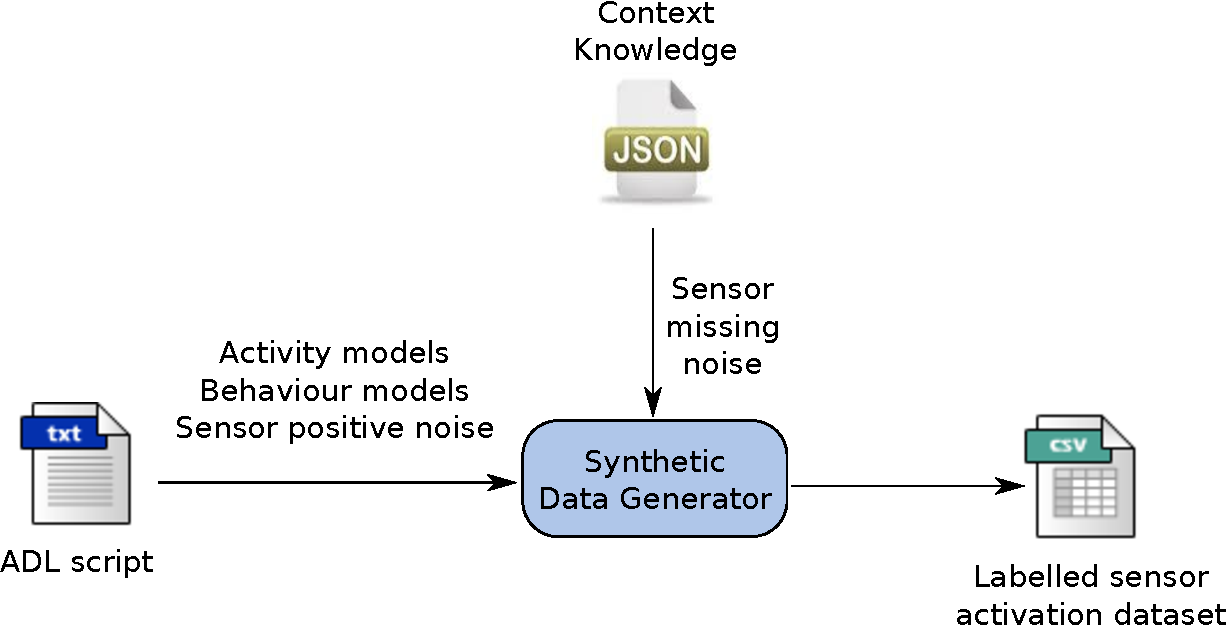
\includegraphics[width=10cm]{synthetic_tool.pdf}
    \caption{High-level design of the synthetic dataset generator tool.}
    \label{fig-synth-tool}
\end{figure}

One of the design decisions was to separate the representation of both sensor error models between two different files. The reason is that sensor missing noise is completely linked to sensor technology and the pervasive infrastructure (wireless receivers, communication, and system sampling and conversion mechanisms), whereas sensor positive noise is more related to environmental aspects, such as the distribution of objects and human behaviour. Hence while sensor missing noise can be considered a property of a sensor, sensor positive noise is more influenced by the inhabitant and the environment. That is why missing error models are included in the context knowledge file depending on the sensor type and positive error models are represented in the ADL script which represents a concrete user.

To make this decision the research carried out by Chen et al. in \cite{Chen2012a} has been considered. They show some experiments for activity recognition in a smart home environment using the dense sensing activity monitoring approach. Throughout the experiment of 144 activities, a total of 804 user-object interactions were performed. They used the so called User-object Interaction Recognition Accuracy (UoIR), defined as the system’s correctly captured interactions against the total occurred interactions, as the metric to evaluate the reliability and performance of the activity monitoring mechanism. This metric takes into account not only unfired or misread interactions caused by faulty sensors but also those circumstances caused by the pervasive infrastructure. As such it is more accurate to reflect the system monitoring performance. Table \ref{tab-sensor-errors} shows the UoIR for different types of sensors with an overall average UoIR of 96.89\%. They conclude that this data proves the monitoring and acquisition mechanism of the system as being very reliable.

\begin{table}[htbp]\scriptsize
\begin{center}
 \begin{tabular}{cccc}
  \hline
  Sensor type & Total interactions & Captured interactions & Accuracy (\%) \\
  \hline
  Contact & 624 & 611 & 97.92 \\
  Tilt & 126 & 119 & 94.44 \\
  Pressure & 36 & 32 & 88.89 \\
  Sound & 18 & 17 & 94.44 \\
  \hline
 \end{tabular}
 \caption{Interaction recognition rate as shown in \cite{Chen2012a}.}
 \label{tab-sensor-errors}
\end{center} 
\end{table}

However, no positive sensor noise has been identified in \cite{Chen2012a}, even though they simulate it in some of their experiments. This is quite reasonable, since the normal state of the sensor represents no interaction. It is very complicated from the technological point of view to change the state of a sensor when no interaction occurs, so it can be concluded that spontaneous sensor activations are very rare. If positive sensor noise is registered, it has to be mainly caused by undesired interactions that actually occur, even though they are not part of the activity. Those undesired interactions can be due to human erratic behaviour (see definition \ref{def-erratic}) or interactions among objects caused by their distribution and casual movements. 

Given that according to literature spontaneous sensor activations are rare and interactions among objects usually occur due to human intervention, it can be concluded that sensor positive noise is mainly caused by user erratic behaviour. Thus it has been included in the ADL script rather than in the contextual knowledge file.

\subsubsection*{ADL script}

The ADL script defines activity models, behaviour models and sensor positive noise for a concrete user. It is currently implemented as a plain text file which has its own syntax. A parser function has been implemented to parse the file and obtain all the models defined on it. 

The first information given in the ADL script refers to the number of days that has to be simulated. A natural number is provided there.

The next part of the file is for defining \textit{sensor activation patterns} for activities. Sensor activation patterns are used to describe how activities are performed in terms of sensor activations and thus represent activity models in terms of sensors. An activity can have an arbitrary number of sensor activation patterns, which are specified with an occurrence probability and a sequence of sensor activations with relative time lapses. An example of sensor activation patterns for activity MakeCoffee can be found in Figure \ref{fig:sensor-act}.

\begin{figure}
\begin{small}
\lstset{linewidth=\textwidth}
\begin{lstlisting}
MakeCoffee 2
0.7 coffeePotSens@0 ktapSens@10 afcoffeeSens@30 cookerSens@20 
    cupSens@180 fridgeSens@10 smilkSens@5 wsugarSens@10
0.3 coffeePotSens@0 ktapSens@10 afcoffeeSens@30 cookerSens@20 
    cupSens@180 wsugarSens@10
\end{lstlisting}
\end{small}
\caption{Sensor activation patterns for MakeCoffee activity obtained from a real user. The activity has two activation patterns with different occurrence probabilities.}
\label{fig:sensor-act}
\end{figure}

First of all, the name of the activity is defined. The number that comes after the name specifies the number of sensor activation patterns for that activity. The next line represents the first sensor activation pattern, which begins with an occurrence probability $p \in [0, 1]$. Notice that the occurrence probabilities of all sensor activations for a given activity must sum to 1. The probability number is followed by a sequence of sensor activations and relative time lapses. The first sensor activation's time has to be 0, indicating that it is the first sensor activation of the activity. The values that come after the '@' symbol represent the time in seconds between the previous sensor activation and the current one. In consequence, in the example given in Figure \ref{fig:sensor-act}, \textit{cookerSens@20} means that sensor activation \textit{cookerSens} occurs 20 seconds after the \textit{afcoffeeSens} sensor activation. The specific way the synthetic dataset generator treats those time lapses will be explained later, when the simulation loop is described.
%The synthetic dataset generator establishes a time lapse with a Gaussian random generator whose mean value is the value specified in the script and the standard deviation is the 25\% of the mean. This way, time lapses between two consecutive sensor activations are realistic. 

Once all activity models are represented using appropriate sensor activation patterns, behaviour models are defined, which represent different days of the user in terms of performed activities (see definition \ref{def-behaviour}). Two kinds of behaviour models are defined: 

\begin{enumerate}
 \item \textbf{Sequences:} where a time slot is given with a sequence of activities and relative time lapses between two consecutive activities. Sequences are used to define those activity sequences that are always performed by a user in concrete days.
 \item \textbf{Alterations:} where a probability value is assigned to an activity to be performed in a concrete time slot. Alterations represent a different kind of behaviour model. Some users might perform an activity regardless of the week day. For example, a user might watch television in evenings with a certain probability. Some days the user watches television, but some days does not. It does not depend on the day, but on some other causes (mood, last hour plans, etc.).
\end{enumerate}

Specific week days are not represented in behaviour models. Instead of that, the probability of a concrete list of sequences and alterations is given. A list of sequences and alterations models a day. So if such a day model occurs 2 days in a week, i.e. in weekends, the assigned probability will be $2/7 \simeq 0.29$. An example is depicted in Figure \ref{fig:activity-pattern}. A typical day of a user is described, with an occurrence probability of 0.29, since the activity pattern describes a weekend day. In this case, the user reported that (s)he sometimes reads a book in the afternoon. Alterations allow modelling this kind of behaviour.


\begin{figure}
\begin{small}
\lstset{linewidth=\textwidth}
\begin{lstlisting}
Prob 0.29 4
S 9:00-10:00 MakeCoffee@0 BrushTeeth@1800 ReadBook@120
S 13:30-14:30 MakePasta@0 BrushTeeth@600
S 22:00-23:00 BrushTeeth@0 WashHands@10
A 18:00-20:00 ReadBook 0.5
\end{lstlisting}
\end{small}
\caption{An example of a behaviour model for a concrete day, which has an occurrence probability of 0.29 and it is composed of three sequences and an alteration.}
\label{fig:activity-pattern}
\end{figure}

As it happens with sensor activation patterns, the occurrence probabilities of behaviour models must sum to 1.

The last part of the script is to define sensor positive noise (see definition \ref{def-positive}). As sensor positive noise is mainly caused by user erratic behaviour it is very complex to model it accurately. Besides, obtaining those models from user surveys is impossible, since users cannot tell how they interact with objects unpurposely. For those reasons, a simple sensor error model has been adopted which guarantees noise generation independently from ongoing activities. A probability value can be assigned to concrete sensors to get activated in an hour interval using a uniform probability distribution. For example, sensor \textit{cupSens} can be assigned an activation probability of 0.1, which means that each hour, the sensor has a 0.1 probability of getting activated. 

\subsubsection*{Context knowledge file}

The context knowledge file has been described in Section \ref{subsec:approach:inputs}, where an example of such a file was provided in Figure \ref{fig-context-json}. But sensor missing noise models were not shown in that example. As sensor missing noise is mainly related to the sensor type, another part is added to the context knowledge file. More concretely, Figure \ref{fig-missing-noise} shows an example of how such error models are implemented for contact and tilt sensors. For each sensor type, a missing probability $p \in [0, 1]$ is provided. 

\begin{figure}[htbp]
\begin{small}
\begin{lstlisting}
"error_models": {
   "contact": {
	"prob": 0.0208
   },
   "tilt": {
	"prob": 0.0556
  },
  ...
}
\end{lstlisting}
\end{small}
\caption{Example of sensor missing noise models for contact and tilt sensors.}
\label{fig-missing-noise}
\end{figure}

In consequence, the context knowledge file has the information about activities, objects, sensors and sensor missing noise models. It is mandatory for the synthetic dataset generator to keep the coherence between the sensors used in the ADL script and in the context knowledge file. The tool itself makes sure that coherence exists. If there is a sensor activation in the ADL script which is not represented in the context knowledge file, the synthetic dataset generator raises an error.

\subsubsection*{Simulation loop}

Using the ADL script and the context knowledge file, the synthetic dataset generator creates a CSV file where each sensor activation has an associated timestamp and is labelled with an activity name or with the special label None if it is caused by noise. Additionally, activity start and end times are marked in the dataset.

For the purpose of generating realistic sensor activation datasets, the synthetic dataset generator has a simulation loop which has been represented in a flowchart in Figure \ref{fig-sim-loop}. First of all, the simulator fixes the first day to start the simulation. In the current implementation the same day the simulator is launched is used as the first day. Afterwards, for the selected day, sensor positive noise is generated. For that purpose, the simulator generates a random number per each sensor with a probability greater than zero. If the sensor has to be activated, the simulator chooses a concrete time inside the current hour using a uniform distribution. The process finishes when the 24 hours of the day have been treated.

\begin{figure}[htbp]
\centering
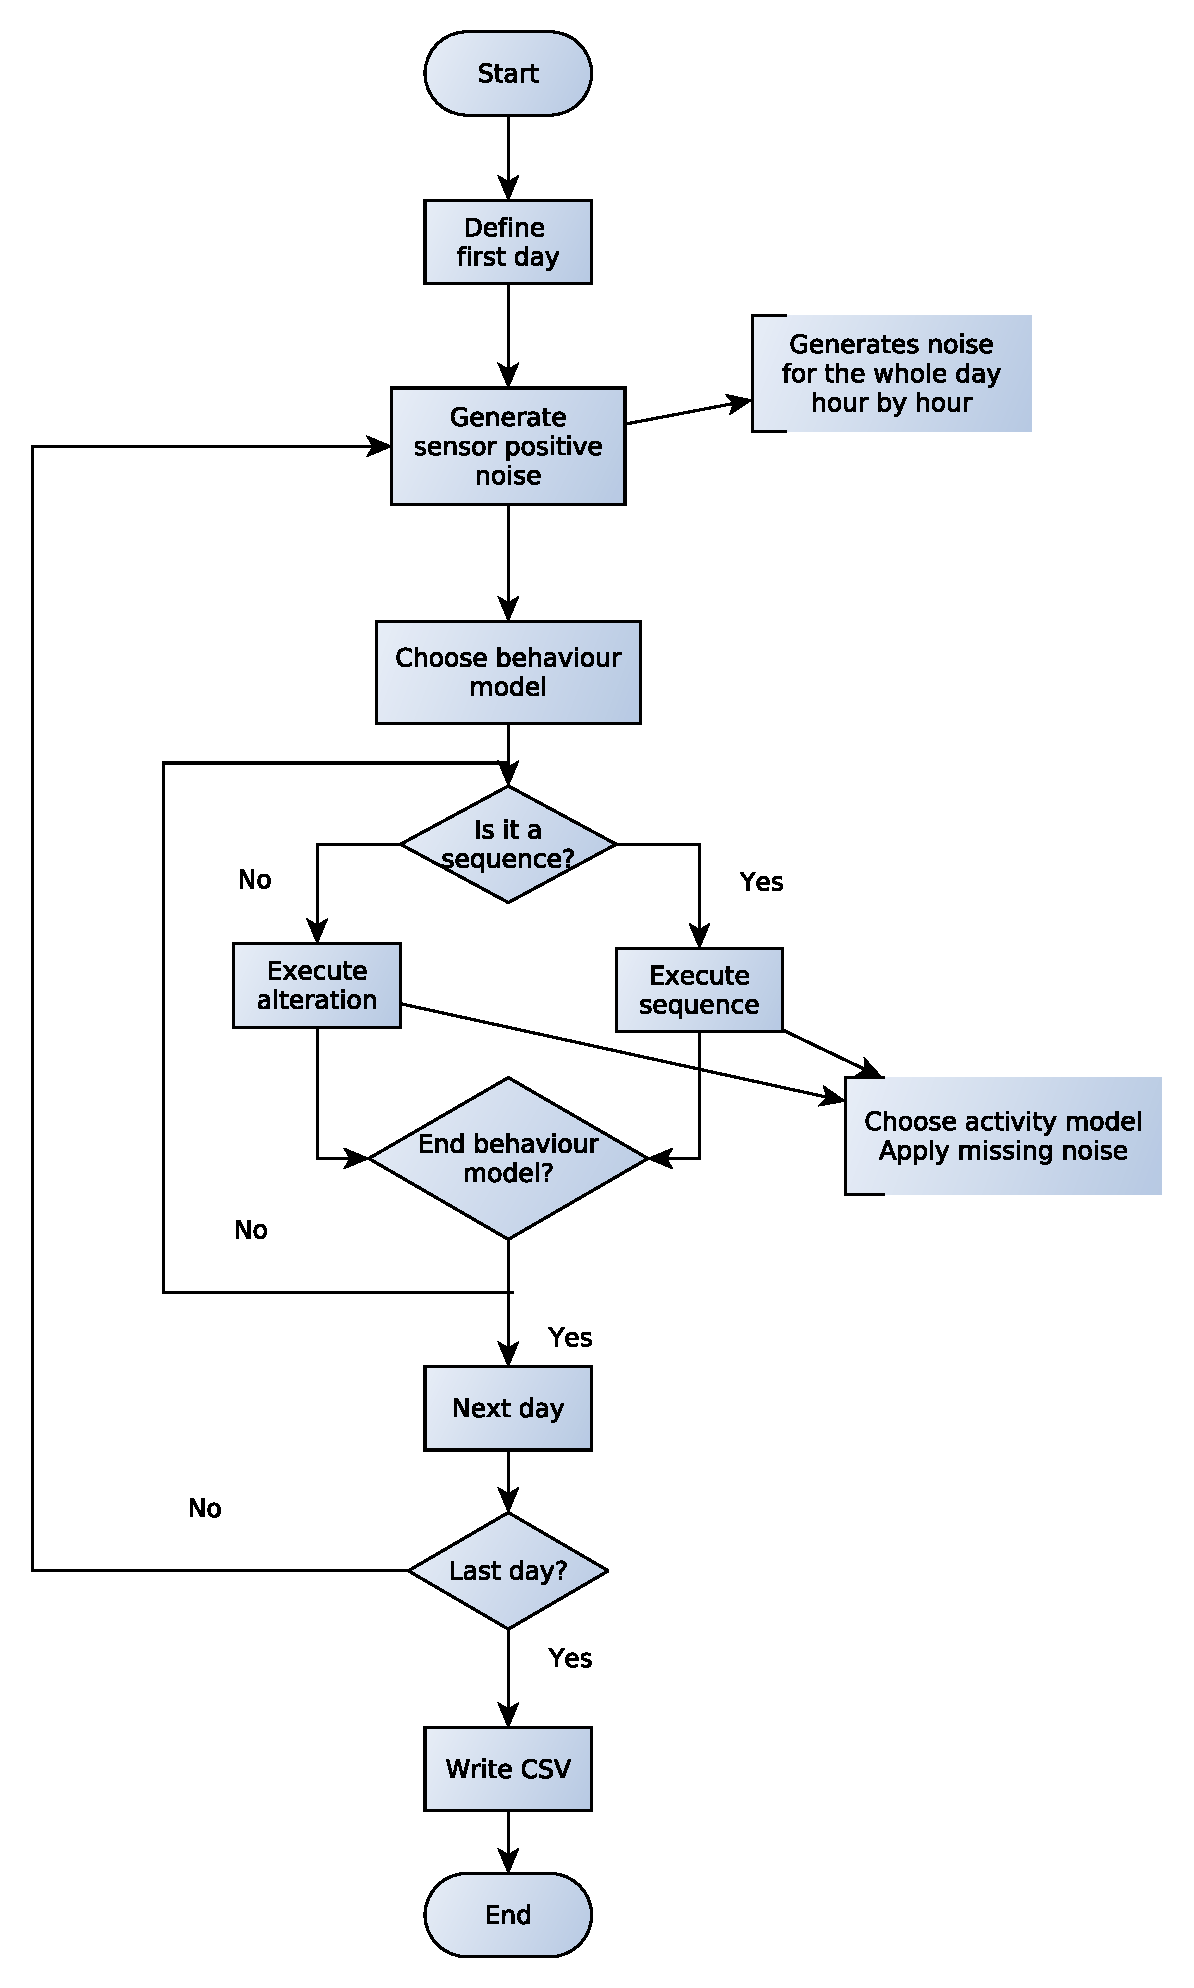
\includegraphics[width=11cm]{simulation_loop.pdf}
    \caption{A flowchart of the simulation loop of the synthetic dataset generator.}
    \label{fig-sim-loop}
\end{figure}

Once sensor positive noise has been generated for the whole day, a behaviour model is chosen, taking into account the probabilities of each model. The behaviour model is a list of sequences and alterations. The first element of the list is taken. If it is a sequence, the activities of the sequence are executed in the specified time slot. For example, assume the sequence is such that 

\begin{small}
\begin{lstlisting}
 S 9:00-10:00 MakeCoffe@0 WatchTelevision@30 BrushTeeth@1800 
\end{lstlisting}
\end{small}

\noindent In that case, the simulator generates a start time for the sequence in the provided time slot, using a uniform distribution. Afterwards, it picks the first activity (MakeCoffee) and looks for the sensor activation patterns of that activity. The simulator probabilistically chooses one of the sensor activation patterns of the activity and executes it. While executing the activity itself, two main aspects are taken into account:

\begin{enumerate}
 \item Time lapses between sensor activations: the time lapses provided in the script are used as the mean values of Gaussian distributions, whose standard deviation is fixed to a 25\% of the mean by default. So the time lapse is generated probabilistically using as reference the value given in the script. This makes varying and realistic time lapses for consecutive sensor activations.
 \item Sensor missing noise: before generating the sensor activation, its missing probability is consulted in the context file. The simulator uses the missing probability to decide whether to generate the activation.
\end{enumerate}

Similarly to sensor activations, time lapses between activities are treated through Gaussian distributions. At the end of the process, the whole sequence will be executed, with probabilistically chosen time lapses and sensor missing errors.

To execute an alteration, the simulator uses its occurrence probability. If it has to be executed, the activity is performed as in sequences. When the behaviour model is fully executed, i.e. all the elements of the list have been treated, the simulator generates the next day and repeats the whole process until the last day is reached. When this happens, the generated dataset is written in a CSV file, where properly labelled timestamped sensor activations can be found.

\subsection{Discussion about the hybrid methodology}
\label{subsec:evaluation:hybrid:discussion}
\begin{comment}
- Explain the advantages: generate virtually infinite datasets, arbitrary number of days, perfectly labelled, sensor noise, erratic behaviour, realistic time lapses
 - Explain the main disadvantages: erratic behaviour difficult to capture
 \end{comment}
The hybrid methodology explained in Section \ref{subsec:evaluation:hybrid} is based on the limitations and solutions identified in the literature \cite{Helal2011} \cite{Helal2012} \cite{Okeyo2012a}. It has been specially designed to evaluate the EAM learning system and thus, it has some specific tools to adapt the methodology to the constraints of the system. However, the methodology itself, apart from concrete implementations, can be used to evaluate other activity recognition systems and has several advantages over the standard methodology explained in the beginning of Section \ref{sec:evaluation:methodology}. Let us enumerate and justify the advantages:

\begin{enumerate}
 \item The hybrid methodology is cost effective, both from economic and time perspectives: from the economic point of view, the hybrid methodology does not need any pervasive environment, which can become an important investment. Furthermore, the cost of the experiments is also avoided, such as paying to participants, preparations etc. From the time point of view, savings can be very important too, specially if a high number of experiments is planned. Preparing, distributing and processing surveys among users needs a variable amount of time, but it is unarguably less than preparing and running real experiments with humans. 
 \item A lot of users' information can be used: as it is based on surveys, it is generally easy to achieve a great number of users for the tests, in contrast with what happens using the standard methodology. When running experiments with humans, finding volunteers is usually very difficult, specially if the experiment is long in time. 
 \item Ethical and legal issues are much softer: as there are no experiments with human beings many ethical and legal aspects can be avoided. The only important point to be considered is the anonymity of users regarding the information they provide in the surveys.
 \item Datasets can be generated on demand: using the synthetic dataset generator or any other convenient simulator, arbitrary number of datasets can be generated as needed.
 \item Perfectly labelled datasets can be obtained: the synthetic dataset generator labels all sensor activations according to the given script and sensor error models. In consequence, the generated dataset is a perfect ground truth. On the other hand, when using the standard methodology, dataset annotation is a real issue. As noted by Rashidi and Cook in \cite{Rashidi2011}: \blockquote{\textit{An aspect of activity recognition that has been greatly under-explored is the method used to annotate sample data that the scientist can use to train the activity model.}} Several annotation methods have been used by researchers, but all of them have their weaknesses. As a consequence, those datasets are not perfectly labelled and they can include spurious sensor activations in activities as ground truth.
 %\item The influence of researchers is minimised: using surveys, researchers cannot write their own scripts with their bias. Even though researchers are still responsible of writing the scripts, following appropriate survey-script translation criteria, researchers' influence in the datasets is minimised.
 \item Any kind of scenarios can be implemented: the synthetic dataset generator allows preparing experiments where no sensor noise exist, where only a concrete kind of sensor noise exists or where conditions are as close as possible to realistic settings. The chance of implementing all those varieties of scenarios allows researchers test deeper their activity recognition systems, since they can see the influence of any factor they consider relevant. 
\end{enumerate}

The core ideas of the hybrid methodology are using surveys to capture user behaviour and simulators to generate synthetic data. The concrete implementations for the EAM learning system are derived from the constraints and features of the system, such as focusing on dense sensing scenarios, single user - single activity scenarios, etc. However, when constraints are different, different tools can be used inside the same evaluation methodology. 

In this case, the constraints and features of the EAM learning system make feasible the usage of surveys and simulators. The dense sensing paradigm for activity monitoring establishes that user-object interactions are monitored through simple sensor activations, which are used for activity modelling. So sensor activations are boolean valued, making simulation much easier. For example, Persim introduces sensor value generation functions, because the simulated sensors are broader and can produce different values depending on the context. 

Another simplification comes from the activity modelling approach, which is based on action sequences mapped from sensor activations which monitor objects. This means that sensors like thermometers, humidity sensors, etc. do not have to be modelled and simulated for the EAM learning system. Only sensors attached to objects. The same activity modelling approach makes feasible obtaining accurate activity models from users, since it is easy for any user to describe what objects are used to perform activities. 

The single user - single activity constraint also simplifies the whole evaluation process. Firstly, users do not have to provide information about overlapping and concurrent activities, which is very complicated. Additionally, activity models and behaviour models are kept simple for simulation. Modelling and simulating concurrent activities is a challenge that is avoided in this case. 

Finally, time lapses between actions and activities can also be simulated appropriately, as shown by Okeyo et al. \cite{Okeyo2012a}. Users report approximate time lapses in the surveys and the synthetic dataset generator uses Gaussian random number generators in order to generate user based varying time lapses. 

However, there are some disadvantages too and they are mainly related to human behaviour modelling. The first handicap is that modelling user erratic behaviour is complex. It is very difficult for any user to specify what objects (s)he interacts with unpurposely or to say how an activity is aborted because another thing has to be done. The synthetic dataset generator offers a very straightforward way to model this kind of interactions, but it is the researcher who has to assign probability values to specific sensors without having an appropriate way to model user erratic behaviour. The strategy followed in this dissertation is to introduce high levels of random positive noise to compensate the lack of appropriate models. As it will be shown in Section \ref{sec:evaluation:scenarios}, the difference in the number of sensor activations between noiseless and noisy scenarios are greater than 30\% in average, which means that introduced sensor positive noise is more than a third of the original dataset. 

Another disadvantage refers to the information provided in surveys regarding activity models. Some users are very precise in their answers, but some are not. Activity descriptions given by some users might be discarded due to their vagueness. But this is not generally a big problem, since obtaining more answers is usually easy. Some other users may omit important details of activities in their answers, forgetting for example an object which has been used, hence the precise way of performing activities cannot always be captured. This is certainly a problem while modelling activities, but from the EAM learning evaluation perspective, it is a minor problem. The aim of the EAM learning system is to learn activity models which are represented in the datasets. Whether those datasets are really an accurate version of an activity is not that important as far as the learning system captures and models them as they appear.

In consequence, it can be claimed that the hybrid evaluation methodology with its current implementation, is appropriate to evaluate the proposed EAM learning system. Its advantages are many and very important, while the disadvantages can be coped with specific strategies. 


\section{Evaluation Scenarios, Results and Discussions}
\label{sec:evaluation:scenarios}

% divide the tests into two stages:
% 1) Test SA³ with fully simulated conditions -> use the IS'14 paper to extract the scenarios but run them agian, since now location infrence is used. Use activity-based evaluation and argue that this evaluation is important to assess the performance of the clustering initialisation. If the initialisation is bad activity-wise, the next steps will not perform well.
% 2) Test the full EAM learning system in two steps: activity clustering (SA³ + AA -> use action-based evaluation) and the full system (activity clustering + AML -> use model-based evaluation). Use Expert Systems with Applications paper to extract evaluation scenarios, metrics and results.

% In all the cases, explain why we are running such experiments and what we are trying to validate with them. 

Using the tools and methodologies described in Section \ref{sec:evaluation:methodology}, several evaluation scenarios have been prepared to test and validate the most important aspects of the EAM learning system. More concretely, three major evaluation scenarios can be distinguished:

\begin{enumerate}
 \item $SA^3$ evaluation scenarios: $SA^3$ is a very important part of the whole EAM learning system, since it is the initialisation step of the clustering algorithm. The performance of $SA^3$ has to be carefully analysed to understand how it works, its main advantages and strong points as well as its main weaknesses. Remember that $AA$ algorithm works on the results of $SA^3$, adding -or not- actions to the initial action clusters detected by $SA^3$. But if $SA^3$ fails at detecting an activity, $AA$ cannot recover it. Thus, the performance of $SA^3$ in all possible situations is key for the performance of the clustering process and in consequence, the performance of the EAM learning system.
 \item Activity clustering evaluation scenarios: the activity clustering process is the sum of the $SA^3$ and $AA$ algorithms. As a result of the process itself, every sensor activation of a dataset is labelled and several clusters for the defined activities are obtained. Action clusters' quality is directly linked to labelling performance. Remember that those action clusters are finally processed by the $AML$ algorithm to learn extended activity models, so assessing the performance of the clustering process by means of labelled sensor activations is very important.
 \item EAM learning evaluation scenarios: finally, the EAM learning system has to be evaluated. The system is composed by the sequential use of $SA^3$, $AA$ and $AML$. Evaluation scenarios have to be set-up in order to validate that the EAM learning system is able to learn extended activity models for different users. The results obtained in those evaluation scenarios are the most important ones, because they give a clear vision of the performance of the whole system.
\end{enumerate}

\subsection{$SA^3$ performance}
\label{subsec:evaluation:sa3}

\subsubsection{Evaluation scenarios and metrics}
\label{subsubsec:evaluation:sa3:scenarios}
To assess the performance of $SA^3$ exhaustively, the features of the synthetic dataset generator will be used to set up different kinds of scenarios. To prepare those scenarios, surveys will not be used. In the case of $SA³$, the main interest is to measure the performance in presence of increasing noise, activities with several variations, varied order of actions, using IAMs that share the same actions, activity sequences that are very close in time, etc. As $SA^3$ alone is not going to be used for real applications, the usage of surveys is not necessary. $SA^3$ makes sense inside the complete activity clustering algorithm, whose performance will be tested using real users' inputs.

With this purpose, four scenarios have been prepared: 

\begin{enumerate}
 \item The ideal scenario: $SA³$ will be tested in ideal conditions, i.e. there is no sensor noise in the dataset.
 \item Missing sensor noise scenario: increasing missing error probability is introduced to two sensors that are mapped to actions of the IAMs of two activities, to understand how the detection of those activities evolves compared to noiseless activities. It is also important to see whether the missing noise affecting to some activities influence the detection of the others.
 \item Positive sensor noise scenario: increasing positive noise is introduced to assess the performance of $SA³$ in presence of positive noise.
 \item Demanding activities scenario: the fourth scenario tests how $SA³$ performs when IAMs of several activities share many actions among them. 
\end{enumerate}

\begin{figure}
\begin{small}
\lstset{linewidth=\textwidth}
\begin{lstlisting}
MakeCoffee 2
0.5 mugSens@0 smilkSens@20 microwaveSens@20 afcoffeeSens@120 
    wsugarSens@20
0.5 cupSens@0 ktapSens@10 microwaveSens@15 wsugarSens@90 
    afcoffeeSens@30
MakeChocolate 2
0.8 mugSens@0 wmilkSens@20 microwaveSens@20 chocoSens@120
0.2 cookerSens@0 potSens@5 wmilkSens@20 chocoSens@30 
    mugSens@200
MakePasta 2
0.8 potSens@0 ktapSens@20 cookerSens@30 macaroniSens@120 
    ftomatoSens@600
0.2 spaghettiSens@0 potSens@20 ktapSens@25 cookerSens@30 
    baconSens@50 creamSens@600
BrushTeeth 2
0.7 brusherSens@0 toothpasteSens@5 glassSens@30 btapSens@5
0.3 brusherSens@0 toothpasteSens@5 glassSens@30 btapSens@5 
    dentalflossSens@15
WatchTelevision 2
0.5 sofaSens@0 rcontrolSens@5 tvSens@10
0.5 rcontrolSens@0 tvSens@5 sofaSens@5
WashHands 2
0.85 btapSens@0 bsoapSens@15 handcreamSens@40
0.15 btapSens@0 bsoapSens@15
ReadBook 2
0.9 bookbSens@0 bedSens@10 blampSens@5
0.1 bookaSens@0 sofaSens@10
\end{lstlisting}
\end{small}
\caption{Sensor activation patterns for the defined activities.}
\label{fig:basic-script-activities}
\end{figure}

The base of the first three scenarios is an ADL script prepared to offer some common features to all experiments. From the activity models point of view: (i) several variations for every activity, (ii) different probability distributions between activity variations, (iii) varied order of actions in activities and (iv) varied time lapses between consecutive sensor activations. From the behaviour model perspective: (i) different day types, (ii) activities which are very close in time and (iii) combinations of sequences and alterations.

The prepared ADL script reflects all those features and tries to be realistic in the definition of the activity and behaviour models. However, notice that at this point, realism is not important (the following evaluation scenarios will address realism properly). Figure \ref{fig:basic-script-activities} shows the defined seven activities of daily living with all the sensor activation patterns and occurrence probabilities. As it can be seen in the Figure, defined activities are: MakeCoffee, MakeChocolate, MakePasta, BrushTeeth, WatchTelevision, WashHands and ReadBook. Different probability distributions can be found for different activities. For example, MakeCoffee has an even occurrence probability for its two variations (50\% - 50\%). However, ReadBook is very unbalanced (90\% - 10\%). Varied order of actions and time lapses can also be seen in the sensor activation patterns of each activity. Finally, some activities contain a lot of sensor activations - six in the case of MakePasta - whereas some others are very short - WashHands or ReadBook with only two -. In general, activity models reflect all the desired features to test the performance of $SA³$, as identified in the paragraph above.

\begin{figure}
\begin{small}
\lstset{linewidth=\textwidth}
\begin{lstlisting}
Prob 0.43 4
S 7:00-7:30 MakeChocolate@0 BrushTeeth@120 WashHands@30
S 13:00-13:30 MakePasta@0 MakeCoffee@60 BrushTeeth@1800
S 20:00-20:30 MakePasta@0 BrushTeeth@200 ReadBook@150
A 18:00-19:30 WatchTelevision 0.8
Prob 0.28 2
S 7:00-7:30 MakeChocolate@0 BrushTeeth@100 WashHands@30
S 20:30-21:00 BrushTeeth@0 ReadBook@50
Prob 0.29 5
S 9:00-10:00 MakeChocolate@0 WatchTelevision@30 BrushTeeth@1800
S 13:30-14:30 MakePasta@0 BrushTeeth@150
S 22:00-23:00 BrushTeeth@0 WashHands@10
A 15:00-16:00 WatchTelevision 0.75
A 18:00-20:00 ReadBook 0.5
\end{lstlisting}
\end{small}
\caption{Sensor activation patterns for the defined activities.}
\label{fig:basic-script-behaviour}
\end{figure}

Behaviour models defined for the first three evaluation scenarios are depicted in Figure \ref{fig:basic-script-behaviour}. Three typical days are defined with different occurrence probabilities. The first one has three sequences and one alteration. Activity WashHands is very close in time to activity BrushTeeth, for example. The second day type tries to simulate a typical day where the inhabitant spends few time in home, showing a big time difference between both activity sequences. Finally, the third day type contains two alterations and three new activity sequences where some activities are again very close in time.

Another common element of the first three evaluation scenarios is the IAMs of the activities. All seven activities have the same IAMs alongside the three scenarios. Figure \ref{fig:basic-iams} shows the IAMs used for the experiments. It is very important to keep the same IAMs in all the experiments, since IAMs aim at describing incomplete but generic activity models for any user.

\begin{figure}
\begin{small}
\lstset{linewidth=\textwidth}
\begin{lstlisting}
   "MakeCoffee": {
      "type": ["Cooking"],
      "location": ["Kitchen"],
      "IAM": ["hasContainer", "hasCoffee"],
      "duration": 360
   },
   "MakeChocolate": {
      "type": ["Cooking"],
      "location": ["Kitchen"],
      "IAM": ["hasContainer", "hasChocolate"],
      "duration": 500
   },
   "MakePasta": {
      "type": ["Cooking"],
      "location": ["Kitchen"],
      "IAM": ["hasPasta", "useCookingAppliance", 
              "useCookingUtensil"],
      "duration": 1200
   },
   "BrushTeeth": {
      "type": ["Hygiene"],
      "location": ["Bathroom"],
      "IAM": ["hasBrusher", "hasToothpaste", "turnOnTap"],
      "duration": 130
   },
   "WatchTelevision": {
      "type": ["Entertainment"],
      "location": ["Lounge"],
      "IAM": ["hasRemoteControl", "useTV"],
      "duration": 40
   },
   "WashHands": {
      "type": ["Hygiene"],
      "location": ["Bathroom"],
      "IAM": ["turnOnTap", "hasSoap"],
      "duration": 90
   },
   "ReadBook": {
      "type": ["Entertainment"],
      "location": ["Bedroom", "Lounge"],
      "IAM": ["hasBook", "useFurniture"],
      "duration": 30
   } 
\end{lstlisting}
\end{small}
\caption{The IAMs of all seven defined activities for the first three evaluation scenarios.}
\label{fig:basic-iams}
\end{figure}

The fourth evaluation scenario is different from the other three scenarios. The idea is to use some activities whose IAMs share the same actions. For that purpose, and trying to keep the realism, the following seven activities have been defined: MakeCoffee, MakeWhippedCream, MakeTiramisu, BrushTeeth, WatchTelevision, WashHands and ReadBook. The first three activities' IAMs are formed by the same four actions. More concretely:

\begin{small}
\lstset{linewidth=\textwidth}
\begin{lstlisting}
 IAM(MakeCoffee) = {hasContainer, hasCoffee, hasFlavour}
 IAM(MakeWhippedCream) = {hasContainer, hasCream, hasFlavour}
 IAM(MakeTiramisu) = {hasContainer, hasCream, hasCoffee} 
\end{lstlisting}
\end{small}

The other activities are defined as in the previous scenarios. So the aim of this evaluation scenario is to see how $SA³$ behaves with challenging IAMs. To focus only on the pattern recognition performance, no noise is added to this fourth evaluation scenario.

For all four evaluation scenarios the same metrics have been used. The most important aspect for $SA³$ to be evaluated is whether activities are well detected. So labels given to sensor activations are not important. Rather, a comparison between the start and end times of the activity detected by $SA³$ and the real activity has to be done. Assume $A_R$ is the real activity and $A_{SA³}$ the activity detected by $SA³$. $A_{SA³}$ is a correct activity detection if $A_R$ contains $A_{SA³}$ and both activities have the same label:

\begin{equation}
\begin{gathered}
 t_{start}(A_R) \leq t_{start}(A_{SA³}) \mbox{ and } t_{end}(A_{SA³}) \leq t_{end}(A_R) \\
 Label(A_R) = Label(A_{SA³})
\end{gathered}
\label{metric-sa3}
\end{equation}

This evaluation criterion is called \textit{activity-based evaluation}. Using activity-based evaluation criterion, true positives, false positives and false negatives are calculated for every activity, comparing the output of $SA³$ with the ground truth.

\subsubsection{Results}
\label{subsubsec:evaluation:sa3:results}
% Put the tables and graphics here

\paragraph*{Ideal scenario}

To test the performance of $SA^3$ and have a base reference, the ideal scenario has been designed. The ADL script has already been described (Section \ref{subsubsec:evaluation:sa3:scenarios}) and it contains varying order of sensor activations per activity, varied occurrence probability distributions and varied time lapses between sensor activations and activities. The aim of the ideal scenario is to obtain a base reference of the performance of $SA³$ in noiseless conditions. Activity-based evaluation is used and true positives, false positives and false negatives are measured. 

With the objective of getting reliable results, 130 days have been simulated. More concretely, the sensor activation dataset contains 4093 sensor activations describing a total number of 1027 activity instances. The results are shown in Table \ref{tab-sa3-ideal}. For each activity, the number of instances and the percentages of true positives, false positives and false negatives are given.

\begin{table}[htbp]\scriptsize
  \begin{center}
        \begin{tabular}{ccccc}
            \hline            
            \textbf{Activity} & \textbf{Instances} & \textbf{True Positives (\%)} &  \textbf{False Positives (\%)} & \textbf{False Negatives (\%)}\\             
            \hline
            MakeChocolate   & 130 & 100 & 0 & 0 \\
	    WatchTelevision & 103 & 100 & 0 & 0 \\
	    BrushTeeth      & 350 & 100 & 0 & 0 \\
	    WashHands       & 130 & 100 & 0 & 0 \\
	    MakePasta       & 146 & 100 & 0 & 0 \\
	    ReadBook        & 112 & 100 & 0 & 0 \\
	    MakeCoffee      & 56 & 100 & 0 & 0 \\
            \hline
        \end{tabular}                
        \caption{Results of the $SA³$ algorithm for the ideal scenario.}
        \label{tab-sa3-ideal}
    \end{center}
\end{table}

Table \ref{tab-sa3-ideal} shows that the 100\% of all activities are properly captured by $SA³$ under ideal conditions. There are neither false positives nor false negatives. Remember that activity-based evaluation does not check for the labels of every sensor activation. The fact that a 100\% of all activities are properly captured indicates that $SA³$ gets activity time locations robustly.

\paragraph*{Sensor missing noise scenario}

For the next experiments, assessing the performance of $SA³$ under sensor missing error noise is the objective. In principle, the completion criterion of the activity sequence finding step of $SA^3$ suggests that if a sensor activation which is mapped to one of the IAMs fails, $SA³$ would fail to detect that activity (see Section \ref{subsec:clustering:sa3:find} for a detailed explanation). In order to test that suggestion, two of the seven activities have been chosen. Sensor activations which are mapped to the IAMs of those activities are given an increasing missing probability, to see how this missing noise affects the detection of those activities. The rest of the activities are kept noiseless, to measure the effect of missing noise in other activities. Table \ref{tab-sa3-missing} shows the results for the sensor missing noise scenario. The activities which suffer missing noise are marked with an asterisk (MakeChocolate and BrushTeeth). Five experiments are run, each of them simulating 130 days. Sensor missing probabilities are 0.01, 0.02, 0.05, 0.07 and 0.1. For each experiment, true positives, false positives and false negatives are measured, using the activity-based evaluation criterion. 

\begin{table}[htbp]\scriptsize
  \begin{center}
        \begin{tabular}{cccccc}
            \hline            
            \textbf{Activity} & \multicolumn{5}{c}{\textbf{Sensor missing probability}}\\
             & 0.01 & 0.02 & 0.05 & 0.07 & 0.1 \\
             & TP- FP - FN (\%) & TP - FP - FN (\%) & TP - FP - FN (\%) & TP - FP - FN (\%) & TP - FP - FN (\%)\\
            \hline
            MakeChocolate*   & 99.2 - 0 - 0 & 99.2 - 0 - 0 & 94.6 - 0 - 0 & 92.3 - 0 - 0 & 89.2 - 0 - 0 \\
	    WatchTelevision  & 100 - 0 - 0 & 100 - 0 - 0 & 100 - 0 - 0 & 100 - 0 - 0 & 100 - 0 - 0 \\
	    BrushTeeth*      & 98.9 - 0 - 0 & 98.6 - 0 - 0 & 96 - 0 - 0 & 93.8 - 0 - 0 & 89.4 - 0 - 0 \\
	    WashHands        & 100 - 0 - 0 & 100 - 0 - 0 & 100 - 0 - 0 & 100 - 0 - 0 & 100 - 0 - 0 \\
	    MakePasta        & 100 - 0 - 0 & 100 - 0 - 0 & 100 - 0 - 0 & 100 - 0 - 0 & 100 - 0 - 0 \\
	    ReadBook         & 100 - 0 - 0 & 100 - 0 - 0 & 100 - 0 - 0 & 100 - 0 - 0 & 100 - 0 - 0 \\
	    MakeCoffee       & 100 - 0 - 0 & 100 - 0 - 0 & 100 - 0 - 0 & 100 - 0 - 0 & 100 - 0 - 0 \\
            \hline
        \end{tabular}                
        \caption{Results of $SA³$ for the sensor missing noise scenario, where TP: true positives, FP: false positives and FN: false negatives. The activities affected by the noise have an asterisk.}
        \label{tab-sa3-missing}
    \end{center}
\end{table}

As it can be seen in Table \ref{tab-sa3-missing}, the performance of $SA³$ for the rest of activities does not vary. It keeps on producing 100\% of true positives, while false positives and negatives are null. However, true positive rate of activities MakeChocolate and BrushTeeth seems to be linearly reducing with sensor missing noise probability. There is no effect in false positives and negatives, but the effect on true positives is clear, as expected. To make the linearity more clear, Figure \ref{fig:sa3-missing} plots true positive rates for both activities for measured sensor missing noise probabilities. 

\begin{figure}[htbp]
\centering
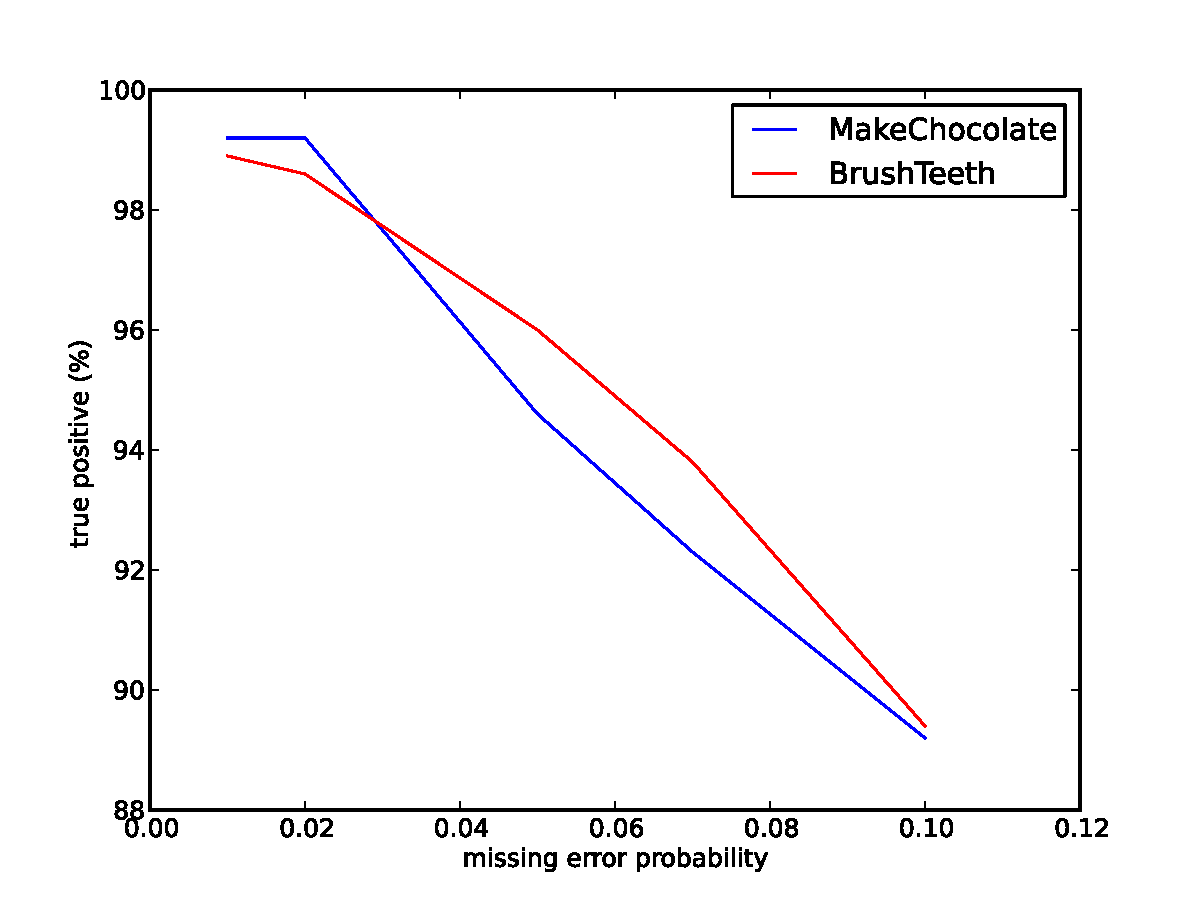
\includegraphics[width=10cm]{missing_error_graphic.pdf}
    \caption{The true positive percentages of $SA^3$ for activities MakeChocolate and BrushTeeth in presence of increasing sensor missing noise.}
    \label{fig:sa3-missing}
\end{figure}

Taking into account that noise generation is probabilistically accomplished in the synthetic dataset generator, Figure \ref{fig:sa3-missing} is a confirmation of the inverse linear relation between sensor missing noise and $SA³$ activity detection performance. When missing error increases, activity detection decreases. 

\paragraph*{Sensor positive noise scenario}

To test the sensor positive noise scenario, five experiments have been run. For each of the experiments, six sensors are picked up randomly and they are assigned increasing sensor positive noise probabilities. This strategy allows measuring the performance of $SA³$ in presence of positive noise. For each of the experiments 130 days are simulated again. To have a reference of the level of noise, sensor activations in each dataset scale from 5054 to 8850. The noiseless scenario presented 4093 sensor activations, so the noisiest dataset contains around 46\% more sensor activations. Table \ref{tab-sa3-positive} shows the results for the sensor positive noise scenario. Each experiment is identified by its noise level, where 0.05 means that all randomly selected sensors have a positive noise probability of 0.05 per hour. For each experiment, true positives, false positives and false negatives are depicted.

\begin{table}[htbp]\scriptsize
    \begin{center}    
        \begin{tabular}{cccccc}
            \hline            
            \textbf{Activity} & \multicolumn{5}{c}{\textbf{Sensor positive probability}}\\
             & 0.05 & 0.1 & 0.15 & 0.2 & 0.25 \\
             & TP - FP - FN (\%) & TP - FP - FN (\%) & TP - FP - FN (\%) & TP - FP - FN (\%) & TP - FP - FN (\%)\\
            \hline
            MakeChocolate   & 100 - 0 - 0 & 100 - 0 - 0 & 100 - 0 - 0 & 100 - 0 - 0 & 100 - 0 - 0 \\
	    WatchTelevision & 100 - 0 - 0 & 100 - 0 - 0 & 99.1 - 0.9 - 0 & 100 - 0 - 0 & 100 - 0 - 0 \\
	    BrushTeeth      & 100 - 0 - 0 & 100 - 0 - 0 & 100 - 0 - 0 & 100 - 0 - 0 & 100 - 0 - 0 \\
	    WashHands       & 100 - 0 - 0 & 100 - 0 - 0 & 100 - 0 - 0 & 100 - 0 - 0 & 100 - 0 - 0 \\
	    MakePasta       & 100 - 0 - 0 & 100 - 0 - 0 & 100 - 0 - 0 & 100 - 0 - 0 & 99.3 - 0.7 - 0 \\
	    ReadBook        & 100 - 0 - 0 & 100 - 0 - 0 & 100 - 2.6 - 0 & 100 - 0 - 0 & 100 - 1.9 - 0 \\
	    MakeCoffee      & 100 - 0 - 0 & 100 - 0 - 0 & 100 - 0 - 0 & 100 - 0 - 0 & 100 - 0 - 0 \\
            \hline
        \end{tabular}          
        \caption{Results of $SA³$ for positive sensor noise scenario; TP: true positives; FP: false positives; FN: false negatives}
        \label{tab-sa3-positive}
    \end{center}
\end{table}

Table \ref{tab-sa3-positive} shows that sensor positive noise affects true positives and false positives. For the first one, a slight reduction for some activities can be seen. For the second one, some activities show rates that even being greater than zero, they are still very low, 2.6\% being the highest for those experiments. Exploring obtained data deeper, it was found that true positive decrease is generated by the appearance of false positives, i.e. in some cases, the false positives are generated overlapped with the real activity, but as they are not contained by the real activity, they are false positives and affect the detection rate. This happens when a sensor activation which is mapped to an action in the IAM of a given activity is generated by chance very close in time from a real execution of that activity. It can be seen in activities WatchTelevision and MakePasta, for example. In some other cases, false positives do not affect true positives (look at ReadBook for 0.15 and 0.25 noise levels). In those cases, the problem is that the IAM of activity ReadBook is composed by two actions: \textit{hasBook} and \textit{useFurniture}. As sensor activations for two sensors monitoring furniture and books were chosen randomly for noise generation, it turned out that both activations were given in such circumstances that they were detected as activities. However, they do not affect any other activity detection.

\paragraph*{Demanding activities scenario}

The final scenario aims at testing $SA³$ under demanding activities. As it has been explained in Section \ref{subsubsec:evaluation:sa3:scenarios}, demanding activities are those which share many common actions in their IAMs. It can be thought that as $SA³$ uses a pattern recognition algorithm where some specific domain-based criteria are applied, its performance could be affected by very similar IAMs. Those conditions are simulated using seven activities, where MakeCoffee, MakeTiramisu and MakeWhippedCream share the same four actions in their IAMs. Remember that even being very similar, they are still different and unique. For this special scenario, a total number of 1262 activity instances have been produced. No sensor noise has been produced for the experiment, since the objective is to see the effect of demanding activities. Obtained results can be seen in Table \ref{tab-sa3-demanding}.

\begin{table}[htbp]\scriptsize
    \begin{center}         
        \begin{tabular}{ccccc}
            \hline
            \textbf{Activity} & \textbf{Instances} & \textbf{True positives (\%)} & \textbf{False positives (\%)} & \textbf{False negatives (\%)} \\
            \hline
            MakeCoffee         & 222 & 100 & 0 & 0 \\
	    MakeTiramisu       & 120 & 100 & 0 & 0 \\
	    MakeWhippedCream   & 72  & 100 & 0 & 0 \\
	    WashHands          & 150 & 100 & 0 & 0 \\
	    BrushTeeth         & 420 & 100 & 0 & 0 \\
	    ReadBook           & 127 & 100 & 0 & 0 \\
	    WatchTelevision    & 151 & 100 & 0 & 0 \\
            \hline
        \end{tabular}  
        \caption{Results of $SA³$ for demanding activity models scenario.}
        \label{tab-sa3-demanding}
    \end{center}
\end{table}

Results show that $SA³$ is not affected by the similarity of IAMs, as long as they are unique. True positives are 100\% for all activities, whereas false positives and negatives are zero. The situation is exactly the same as in the ideal scenario. Notice that assuming unique IAMs for each activity is very reasonable, since if there are two equal IAMs for two activities, those two activities should actually be one. 

\subsubsection{Discussion about SA³}
\label{subsubsec:evaluation:sa3:discussion}

Results shown in Section \ref{subsubsec:evaluation:sa3:results} show that $SA^3$ can handle varying order of actions in activity performance without any problem. All four set-ups contain different activation patterns, where actions are executed in different orders. This can be seen in Figure \ref{fig:basic-script-activities}: every activity has different sensor activation sequences with varying orders. As the ideal scenario shows (Table \ref{tab-sa3-ideal}), the success rate of the algorithm for every activity is 100\% and neither false positives nor negatives are observed. Notice that sensor activation sequences used for each activity contain many actions which are not used to define any of the IAMs, but the algorithm still performs perfectly when detecting activities. Hence, $SA^3$ can also handle non-considered actions.

As far as noisy scenarios regard, results suggest that missing sensor activations cannot be properly handled by the algorithm, when those activations are linked to actions that are used to define IAMs, i.e. if a sensor activation which is mapped to one of the actions used to define the IAM of a concrete activity fails, that activity cannot be detected by $SA³$. The non-captured activities are proportional to the missing activation probability of those actions, as shown in Figure \ref{fig:sa3-missing}. This is due to the completeness criterion used in the second step of $SA^3$, as explained in Section \ref{sec:clustering:sa3}, which demands the presence of all actions in the IAM of an activity to consider an action sequence a valid activity. However, missing sensor noise only affects true positive rates of the activities which are faultily registered by sensors. False positive and negative rates keep behaving as the ideal scenario. Moreover, a non-detection of an activity does not have any other effect on the other activities. Following this reasoning, a good way to minimise the impact of sensor missing noise is to monitor key objects for IAMs using robust sensors such as contact sensors.  

Independently from such robust monitoring strategies, it is reasonable to think whether algorithmic solutions to mitigate sensor missing noise can be adopted. The completion criterion is very restrictive in that sense, but it is also very reasonable, since if not, distinguishing real activity executions from positive noise would be very difficult, specially considering the low number of actions used in the IAMs (see Table \ref{tab-avg-actions-comp-t2}). Further approaches have not been analysed in this dissertation, because the low level of missing sensor noise in real environments makes the detection rates very good. However, some ideas are suggested in Chapter \ref{cha:conclusions} for their future development.

For sensor positive noise, the scenario is different. $SA^3$ has shown to perform reliably even with high levels of noise. For example, even having certain sensors with faulty activation probabilities of 0.25 per hour, average true positive rate over all activities is 99.9\%. Simultaneously, false positive rates are still very low, concretely 0.3\% in average, while false negative rates are 0. False positive activity detections are due to random occurrences of actions in time instants which make them compatible with the duration criterion of an activity. The probability of having such false positives increases as the noise level increases and the number of actions in IAMs decreases. However, the results obtained with the highest level of noise of the experiments show how robust $SA³$ is in such scenarios.

Finally, a test involving challenging activity models showed that as far as activity models are unique, $SA^3$ does not have any problem detecting them. Average true positive rate for all activities is 100\% and false positive and negative rates are 0, as it can be seen in Table \ref{tab-sa3-demanding}. Remember that the experiments for challenging or demanding activity models were performed without any noise. So results suggest that the performance is exactly the same as for the ideal scenario. 

In conclusion, $SA³$ has been tested for all the desired requirements listed in Section \ref{subsubsec:evaluation:sa3:scenarios}. From the activity models point of view: (i) several variations for every activity, (ii) different probability distributions between activity variations, (iii) varied order of actions in activities and (iv) varied time lapses between consecutive sensor activations. From the behaviour model perspective: (i) different day types, (ii) activities which are very close in time and (iii) combinations of sequences and alterations. All those features were present in all four evaluation scenarios, where ideal conditions, noisy scenarios and demanding activity models were also tested. Results suggest that $SA³$ is a very reliable tool to detect activity executions. It does not correctly label all the sensor activations, but it accurately captures activity time locations. Thus, it can be concluded that $SA³$ serves as a initialisation step for an activity clustering process.

\subsection{Activity clustering performance}
\label{subsec:evaluation:clustering}

\subsubsection{Evaluation scenarios and metrics}
\label{subsubsec:evaluation:clustering:scenarios}
Testing the activity clustering algorithm, i.e. $SA³ + AA$, requires the usage of the hybrid evaluation methodology. The activity clustering algorithm can be seen as an activity annotator algorithm which labels each sensor activation with an activity label. Notice that activity annotation and recognition are not the same thing. Activity recognition is performed online, while sensor activations are being generated. But activity annotation happens offline, once all sensor activations have already been produced. So annotating is typically easier than recognising, since it does not have time restrictions. 

Contrary to the evaluation of $SA³$, realism is a key issue when testing activity clustering. That is why the hybrid evaluation methodology is used to set up two evaluation scenarios: the \textit{ideal} and the \textit{complete} scenario. The first one does not contain any sensor noise, which makes easier the annotation process. The complete scenario is closer to reality since it has sensor noise, which makes annotating more demanding. Sensor missing noise errors are obtained from the statistics given in \cite{Chen2012a} and shown in Table \ref{tab-sensor-errors}. Noise error models have been specified depending on sensor type. For example, pressure sensors have a missing probability of around 10\%. This means that whenever the activity script contains a pressure sensor activation, the synthetic dataset generator will perform it with a 90\% of probability. On the other hand, to model sensor positive noise, the strategy introduced in Section \ref{subsec:evaluation:hybrid:discussion} has been followed, i.e. to introduce high levels of random positive noise to compensate the lack of appropriate models for user erratic behaviour. For all experiments, 6 sensors are randomly chosen to assign them a positive noise probability of 0.05 per hour. And other five sensors are also chosen randomly to assign them a 0.1 probability. 

ADL surveys have been circulated among people from DeustoTech - University of Deusto. Target users are researchers, students and professors, with ages ranging from 20 to 60 years old. The circulated ADL survey can be found in the web\footnote{http://goo.gl/etCNyi}. A total number of 12 answers have been received, but 4 of them were discarded because they provided too vague information to model properly the activity and  behaviour models. Thus, 8 real users are finally used for the experiments. 

It is worth to remember that the $AA$ algorithm has three different time metrics (see Section \ref{sec:clustering:ac}). To test which of them is better, all the generated datasets are treated three times, using a different time metric for each experiment.

So the experimental set-up designed consists of: 

\begin{enumerate}
 \item 8 real users.
 \item 7 activities of daily living labelled as MakeCoffee, MakeChocolate, MakePasta, BrushTeeth, WatchTelevision, WashHands and ReadBook. 
 \item 2 scenarios: the ideal scenario and the complete scenario.
 \item 3 executions of the activity clustering process, using the three different time metrics.
\end{enumerate}

Datasets used for the experiments carried out to evaluate activity clustering are available in the web\footnote{http://www.morelab.deusto.es/pub/synthetic\_adl\_datasets/}. As a summary, 16 different datasets can be found there, 2 per user: the datasets for the ideal and the complete scenarios. All datasets simulate 60 days according to the behaviour models provided by each user.

The evaluation criterion in this case, is the so called \textit{action-based evaluation}: compare the labels given by the clustering process to every sensor activation/action with the ground truth produced by the synthetic dataset generator tool by means of true positives, false positives and false negatives. This evaluation criterion assesses the performance of the clustering process as an activity annotator.

\subsubsection{Results}
\label{subsubsec:evaluation:clustering:results}

\paragraph*{Ideal scenario}

The 8 datasets generated from the ADL surveys for the ideal scenario contain around 2128 sensor activations in average. For each of the experiments, the average true positives, false positives and false negatives are depicted per activity. The averages are calculated over the 8 users. A comparison between the actions labelled by $SA^3$ and $AA$ is depicted in the results. Remember that those results cannot be compared to the results shown for $SA³$ evaluation (Section \ref{subsubsec:evaluation:sa3:results}), since evaluation criteria are different. Table \ref{tab-r-ideal-t1} shows the results when simple time distance is used in $AA$ (equation \ref{eq-t1}). Similarly, Table \ref{tab-r-ideal-t2} depicts the results when normalised time distance is applied (see equation \ref{eq-t2}). Finally, Table \ref{tab-r-ideal-t3} shows how the clustering process performs when the dynamic centre normalised time distance is used for the previous activity (see equation \ref{eq-t3}) and the normalised time distance for the next activity.

\begin{table}[htbp]\scriptsize
    \begin{center}    
        \begin{tabular}{ccccccc}
            \hline            
            \textbf{Activity} & \multicolumn{6}{c}{\textbf{Clustering Results}} \\
             & \multicolumn{2}{c}{True Positive (\%)} & \multicolumn{2}{c}{False Positive (\%)} & \multicolumn{2}{c}{False Negative (\%)} \\
             & $SA^3$ & $AA$ & $SA^3$ & $AA$ & $SA^3$ & $AA$ \\
            \hline
            MakeChocolate   & 55.05 & 98.67 & 0    & 0    & 44.95 & 1.33 \\
	    WatchTelevision & 75.12 & 100   & 0    & 0    & 24.88 & 0    \\
	    BrushTeeth      & 90.91 & 96.8  & 0    & 0    & 9.1   & 3.2 \\
	    WashHands       & 74.93 & 99.87 & 0.1  & 13.12  & 25.07 & 0.14 \\
	    MakePasta       & 55.74 & 99.73 & 0    & 0    & 44.26 & 0.27 \\
	    ReadBook        & 89.08 & 100   & 0    & 0    & 10.91 & 0 \\
	    MakeCoffee      & 62.63 & 99.16 & 0    & 0.19 & 37.37 & 0.84 \\
            \hline
        \end{tabular}
        \caption{Average results for 8 users of the clustering process for the ideal scenario using simple time distance.}
        \label{tab-r-ideal-t1}
        \end{center}
\end{table}

\begin{table}[htbp]\scriptsize
  \begin{center}
        \begin{tabular}{ccccccc}
            \hline            
            \textbf{Activity} & \multicolumn{6}{c}{\textbf{Clustering Results}} \\
             & \multicolumn{2}{c}{True Positive (\%)} & \multicolumn{2}{c}{False Positive (\%)} & \multicolumn{2}{c}{False Negative (\%)} \\
             & $SA^3$ & $AA$ & $SA^3$ & $AA$ & $SA^3$ & $AA$ \\
            \hline
            MakeChocolate   & 55.05 & 98.67 & 0    & 0    & 44.95 & 1.33 \\
	    WatchTelevision & 75.12 & 100   & 0    & 0    & 24.88 & 0    \\
	    BrushTeeth      & 90.91 & 96.57 & 0    & 0    & 9.1   & 3.43 \\
	    WashHands       & 74.93 & 99.86 & 0.1  & 14.27 & 25.07 & 0.14 \\
	    MakePasta       & 55.74 & 99.8  & 0    & 0    & 44.26 & 0.2 \\
	    ReadBook        & 89.08 & 100   & 0    & 0    & 10.91 & 0 \\
	    MakeCoffee      & 62.63 & 99.16 & 0    & 0    & 37.37 & 0.84 \\
            \hline
        \end{tabular}
        \caption{Average results for 8 users of the clustering process for the ideal scenario using normalised time distance.}
        \label{tab-r-ideal-t2}
        \end{center}
\end{table}

\begin{table}[htbp]\scriptsize
    \begin{center}    
        \begin{tabular}{ccccccc}
            \hline            
            \textbf{Activity} & \multicolumn{6}{c}{\textbf{Clustering Results}} \\
             & \multicolumn{2}{c}{True Positive (\%)} & \multicolumn{2}{c}{False Positive (\%)} & \multicolumn{2}{c}{False Negative (\%)} \\
             & $SA^3$ & $AA$ & $SA^3$ & $AA$ & $SA^3$ & $AA$ \\
            \hline
            MakeChocolate   & 55.05 & 98.67 & 0    & 0    & 44.95 & 1.33 \\
	    WatchTelevision & 75.12 & 100   & 0    & 0    & 24.88 & 0    \\
	    BrushTeeth      & 90.91 & 98.27 & 0    & 0    & 9.1   & 1.73 \\
	    WashHands       & 74.93 & 99.72 & 0.1  & 5.1  & 25.07 & 0.27 \\
	    MakePasta       & 55.74 & 99.8  & 0    & 0.04 & 44.26 & 0.2 \\
	    ReadBook        & 89.08 & 100   & 0    & 0    & 10.91 & 0 \\
	    MakeCoffee      & 62.63 & 99.09 & 0    & 0    & 37.37 & 0.91 \\
            \hline
        \end{tabular}
        \caption{Average results for 8 users of the clustering process for the ideal scenario using dynamic normalised time distance for previous and normalised time distance for next activity.}
        \label{tab-r-ideal-t3}
    \end{center}
\end{table}

To get a clearer comparison between three time metrics, Table \ref{tab-r-comparative-ideal} shows the average precision and recall for each time metric. The average is calculated over all activities. As it can be seen, both precision and recall are very high for all three time metrics. However, the combination of dynamic centre normalised and normalised time distances yields the best results, specially for precision. The difference for recall is not very significant. 

\begin{table}[htbp]\scriptsize
\begin{center}
 \begin{tabular}{ccc}
  \hline
   & Avg. Precision & Avg. Recall \\
  \hline
  t1 & 98.12\% & 99.17\% \\
  t2 & 97.98\% & 99.15\% \\
  t3 & 99.26\% & 99.36\% \\
  \hline
 \end{tabular}
 \caption{Comparative between the usage of the three time metrics for the clustering process in the ideal scenario. t1 refers to simple time distance, t2 to normalised time distance and t3 to using dynamic centre normalised time distance for previous activity and normalised time distance for next activity.}
 \label{tab-r-comparative-ideal}
\end{center} 
\end{table}

\paragraph*{Complete scenario}

The 8 datasets for the complete scenario are obtained from the same ADL surveys and scripts. But for these datasets, sensor error models are applied. As a result, datasets have an average of around 2942 sensor activations. Compared to the ideal scenario, those datasets have 38.25\% more sensor activations, which gives a clear idea of the high level of sensor positive noise. Notice that this increment comes even having missing errors, which are applied to every sensor activation. The combination of missing and positive noise gives datasets containing 38.25\% more sensor activations, thus sensor positive noise is very high. 

Results are shown in the same manner as for the ideal scenario. As such, Table \ref{tab-r-comp-t1} shows the results when using simple time distance, Table \ref{tab-r-comp-t2} when using normalised time distance and finally, Table \ref{tab-r-comp-t3} when combining dynamic centre normalised and normalised time distances. Once again, a summary of the performance of the three variants is depicted in Table \ref{tab-r-comparative-complete}, where average precision and recall are shown.
       
\begin{table}[htbp]\scriptsize
  \begin{center}
        \begin{tabular}{ccccccc}
            \hline            
            \textbf{Activity} & \multicolumn{6}{c}{\textbf{Clustering Results}} \\
             & \multicolumn{2}{c}{True Positive (\%)} & \multicolumn{2}{c}{False Positive (\%)} & \multicolumn{2}{c}{False Negative (\%)} \\
             & $SA^3$ & $AA$ & $SA^3$ & $AA$ & $SA^3$ & $AA$ \\
            \hline
            MakeChocolate   & 54.73 & 97.76 & 1.2  & 2.86 & 45.27 & 2.24 \\
	    WatchTelevision & 71.13 & 100   & 0    & 0    & 28.87 & 0    \\
	    BrushTeeth      & 91.18 & 96.97 & 0.28 & 0.41 & 8.82  & 3.03 \\
	    WashHands       & 75.12 & 98.45 & 0.69 & 12.6 & 24.88 & 1.55 \\
	    MakePasta       & 53.88 & 99.7  & 1.34 & 5.2  & 46.12 & 0.29 \\
	    ReadBook        & 82.91 & 94.66 & 0.45 & 0.3  & 17.09 & 5.34 \\
	    MakeCoffee      & 59.14 & 99.83 & 1.32 & 3.23 & 40.86 & 0.17 \\
            \hline
        \end{tabular}
        \caption{Average results for 8 users of the clustering process for the complete scenario using simple time distance.}
        \label{tab-r-comp-t1}
        \end{center}
\end{table}



\begin{table}[htbp]\scriptsize
  \begin{center}
        \begin{tabular}{ccccccc}
            \hline            
            \textbf{Activity} & \multicolumn{6}{c}{\textbf{Clustering Results}} \\
             & \multicolumn{2}{c}{True Positive (\%)} & \multicolumn{2}{c}{False Positive (\%)} & \multicolumn{2}{c}{False Negative (\%)} \\
             & $SA^3$ & $AA$ & $SA^3$ & $AA$ & $SA^3$ & $AA$ \\
            \hline
            MakeChocolate   & 54.73 & 97.76 & 1.2  & 2.86 & 45.27 & 2.24 \\
	    WatchTelevision & 71.13 & 100   & 0    & 0    & 28.87 & 0    \\
	    BrushTeeth      & 91.18 & 96.7  & 0.28 & 0.41 & 8.82  & 3.3 \\
	    WashHands       & 75.12 & 98.45 & 0.69 & 13.99  & 24.88 & 1.55 \\
	    MakePasta       & 53.88 & 99.83 & 1.34 & 5.2 & 46.12 & 0.17 \\
	    ReadBook        & 82.91 & 94.66 & 0.45 & 0.3  & 17.09 & 5.34 \\
	    MakeCoffee      & 59.14 & 99.83 & 1.32 & 2.9  & 40.86 & 0.17 \\
            \hline
        \end{tabular}
        \caption{Average results for 8 users of the clustering process for the complete scenario using normalised time distance.}
        \label{tab-r-comp-t2}
    \end{center}
\end{table}


        
        
\begin{table}[htbp]\scriptsize
  \begin{center}
        \begin{tabular}{ccccccc}
            \hline            
            \textbf{Activity} & \multicolumn{6}{c}{\textbf{Clustering Results}} \\
             & \multicolumn{2}{c}{True Positive (\%)} & \multicolumn{2}{c}{False Positive (\%)} & \multicolumn{2}{c}{False Negative (\%)} \\
             & $SA^3$ & $AA$ & $SA^3$ & $AA$ & $SA^3$ & $AA$ \\
            \hline
            MakeChocolate   & 54.73 & 97.76 & 1.2  & 2.64 & 45.27 & 2.24 \\
	    WatchTelevision & 71.13 & 100   & 0    & 0    & 28.87 & 0    \\
	    BrushTeeth      & 91.18 & 98.43 & 0.28 & 0.41 & 8.82  & 1.57 \\
	    WashHands       & 75.12 & 98.37 & 0.69 & 4.55 & 24.88 & 1.63 \\
	    MakePasta       & 53.88 & 99.39 & 1.34 & 5.62 & 46.12 & 0.61 \\
	    ReadBook        & 82.91 & 94.66 & 0.45 & 0.3  & 17.09 & 5.34 \\
	    MakeCoffee      & 59.14 & 99.24 & 1.32 & 2.6  & 40.86 & 0.76 \\
            \hline
        \end{tabular}
        \caption{Average results for 8 users of the clustering process for the complete scenario using dynamic normalised time distance for previous and normalised time distance for next activity.}
        \label{tab-r-comp-t3}
   \end{center}
\end{table}

\begin{table}[htbp]\scriptsize
\begin{center}
 \begin{tabular}{ccc}
  \hline
   & Avg. Precision & Avg. Recall \\
  \hline
  t1 & 96.71\% & 98.19\% \\
  t2 & 96.59\% & 98.17\% \\
  t3 & 97.75\% & 98.26\% \\
  \hline
 \end{tabular}
 \caption{Comparative between the usage of the three time metrics for the clustering process in the complete scenario. t1 refers to simple time distance, t2 to normalised time distance and t3 to using dynamic center normalised time distance for previous activity and normalised time distance for next activity.}
 \label{tab-r-comparative-complete}
\end{center} 
\end{table}

\subsubsection{Discussion about the clustering process}
\label{subsubsec:evaluation:ac:discussion}

The first discussion point for the clustering process is the difference in performance of the three time metrics. Tables \ref{tab-r-comparative-ideal} and \ref{tab-r-comparative-complete} show a clear comparative, both in the ideal and complete scenario. It can be seen that the difference between simple time distance and normalised time distance is not significant. But using dynamic centre normalised time distance for previous activity and normalised time distance for next activity, yields better results. Notice that even though differences are not very big, the higher precision of the third approach is due to lower false positive rates. For some activities, the first two approaches produce even higher true positives, but at the expense of generating much more false positives. Recall values are very similar for all three time metrics in both scenarios. So it can be claimed that as far as sensor activation labelling regards, combining the dynamic centre normalised time distance and normalised time distance is the best option.

The small differences between three time approaches shown in Tables \ref{tab-r-comparative-ideal} and \ref{tab-r-comparative-complete} means that for outsider actions, the candidate function solves the vast majority of the cases (equation \ref{eq-candidate}). For those outsiders that cannot be classified by the candidate function, the three time metrics play a role. But their effect is minimised because of the low number of such outsiders.

For the rest of the discussion about the clustering process, the third time approach will be considered, since it is the best approach. Tables \ref{tab-r-ideal-t2} and \ref{tab-r-comp-t2} show the good performance of the activity clustering process using context knowledge. True positive rate is very high for all activities. The lowest rate is found for activity ReadBook in the complete scenario: 94.6\%. This is due to two factors: (i) the missing sensor probability for pressure sensors is around 10\% and (ii) the IAM for ReadBook has the action \textit{useFurniture} ($IAM(ReadBook) = \{hasBook, useFurniture\}$); all the objects that are mapped to action \textit{useFurniture} are monitored by pressure sensors, for example, sofa, chair or bed. When pressure sensors fail, $SA^3$ cannot detect the activity and hence, true positive rate decreases. Notice that this happens only because the missing action is part of the IAM of the activity. All other activities, even in the complete scenario, show true positive rates higher than 97\%, reaching in some cases 100\% rates. Those high rates are accompanied with very low rates of false positives and negatives. For example, the highest false positive rate has been found for activity MakePasta in the complete scenario with 5.6\%. 

It is worth to point out the behaviour of the clustering process, divided into two steps. Tables \ref{tab-r-ideal-t2} and \ref{tab-r-comp-t2} show how $SA^3$ labels correctly varying number of sensor activations. This number depends on the relation between the number of sensor activations performed by a user and the number of actions in the IAMs. For instance, if the IAM of activity $A$ has two actions and a concrete user performs in average 9 actions for that activity, $SA^3$ will only label correctly those actions that lie inside the two actions of the IAM. It can be seen that for low action number activities like BrushTeeth and ReadBook, $SA^3$ shows quite a high true positive rate and low false negative rate. However, activities like MakeChocolate or MakePasta have a true positive rate below 60\% and high false negative rates. In any case, in the second step run by $AA$, true positives rise, false negatives get very low and false positives slightly increase, giving similar results for all activities. This means that $SA^3$ discovers activities' time locations very accurately and $AA$ treats insider and outsider actions properly to achieve very good rates building on the results of $SA^3$.

As a conclusion, the clustering process depends on the results of $SA³$, its initialisation step. As such, the clustering process is sensitive to sensor missing noise which affects to actions used in IAMs. However, the complete scenario shows sensor missing noise levels extracted from real deployments and results are very good. Notice that experiments are carried out for eight real users, each of them executing activities in many different ways. The high true positive rates and low false positive and negative rates obtained in such realistic set-ups suggest that the activity clustering process annotates very accurately each sensor activation and thus, action, giving as a result robust action clusters, even in noisy scenarios. Remember that while sensor missing noise models have been extracted from real deployments, sensor positive noise has been exaggerated in order to provide very challenging conditions. Even in those conditions, many of the built action clusters will correspond to real activity models, and some others will contain spurious actions, due to false positive annotations. But looking at the low rate of false positives, it can be concluded that correct action clusters will be dominant. 

\subsection{EAM learning performance}
\label{subsec:evaluation:eam}

\subsubsection{Evaluation scenarios and metrics}
\label{subsubsec:evaluation:eam:scenarios}

%Same evaluation scenarios as in the previous experiments.
For the evaluation of the EAM learning system, the same datasets used and described for the evaluation of the activity clustering system have been used (see Section \ref{subsubsec:evaluation:clustering:scenarios}). The idea is to run the $AML$ algorithm on the clusters extracted by the activity clustering process, using the same activity datasets for the same 8 real users. In consequence, the evaluation scenarios are exactly the same, but they are summarised for convenience:

\begin{enumerate}
 \item 8 real users.
 \item 7 activities of daily living labelled as MakeCoffee, MakeChocolate, MakePasta, BrushTeeth, WatchTelevision, WashHands and ReadBook. 
 \item 2 scenarios: the ideal scenario and the complete scenario.
 \item 3 executions of the activity clustering process, using the three different time metrics. $AML$ is posteriorly executed on all three clustering processes independently.
\end{enumerate}

The chosen evaluation criterion to assess the performance of the EAM learning system is named \textit{model-based evaluation}. It compares the learned activity models with the models provided by users in their answers to the survey. Activity models are compared action-wise, i.e. if a user states that activity $A$ is performed by action sequences $S_1$ and $S_2$, those sequences constitute the ground truth. The sequences resulting from the learning process (clustering process + $AML$) are compared with this ground truth. In this example, it should be checked whether the learning process learns $S_1$ and $S_2$ for activity $A$. The indicators used to show the performance of the EAM learning system are: learned correct action sequences, learned spurious action sequences and learned total action sequences.

Using the described evaluation scenarios and criterion, the EAM learning system's capability of learning activity models is measured. For all experiments, IAMs have been defined previously and they are always the same. Indeed, the IAMs defined in Figure \ref{fig:basic-iams} are the ones used for those experiments. This is important, since IAMs aim at being generic and incomplete activity models for every user. Using those IAMs, the EAM learning system should be able to learn extended activity models for the defined activities, and those models should be the same as the models provided by the users in their surveys. Such results would proof the main claim of this dissertation, i.e. complete and specialised activity models can be learned from user generated data for previously defined incomplete activity models.

\subsubsection{Results}
\label{subsubsec:evaluation:eam:results}

\paragraph*{Ideal scenario}

The datasets used for those experiments have already been described in Section \ref{subsubsec:evaluation:clustering:scenarios}. Remember that the ideal scenario does not contain any sensor noise. $AML$ is run, taking as inputs the results of the clustering process generated in Section \ref{subsubsec:evaluation:clustering:results}. Thus, Table \ref{tab-rp-ideal-t0} shows the results for the ideal scenario using the simple time distance in the clustering process. Analogously, Tables \ref{tab-rp-ideal-t1} and \ref{tab-rp-ideal-t2} show the results in the same scenario, but applying the normalised time distance in the first and the combination of the dynamic centre normalised distance and normalised distance in the second. 


\begin{table}[htbp]\scriptsize
  \begin{center}
        \begin{tabular}{ccccc}
            \hline            
            \textbf{Activity} & \multicolumn{3}{c}{\textbf{Learning Results}} & \textbf{Average Number of Patterns} \\
             & Correct Models & Spurious Models & Total Models & \\
            \hline
            MakeChocolate   & 1    & 0     & 0  & 1 \\
	    WatchTelevision & 1.14 & 0     & 0  & 1.14    \\
	    BrushTeeth      & 1.25 & 0.31  & 0  & 1.25 \\
	    WashHands       & 1    & 0.37  & 0  & 1 \\
	    MakePasta       & 2    & 0     & 0  & 2 \\
	    ReadBook        & 1.12 & 0     & 0  & 1.12  \\
	    MakeCoffee      & 1.71 & 0.24  & 0  & 1.71  \\
            \hline
        \end{tabular}
        \caption{Average results for 8 users of the EAM learning process for the ideal scenario, using the simple time distance in the clustering process.}
        \label{tab-rp-ideal-t0}
    \end{center}
\end{table}


\begin{table}[htbp]\scriptsize
  \begin{center}
        \begin{tabular}{ccccc}
            \hline            
            \textbf{Activity} & \multicolumn{3}{c}{\textbf{Learning Results}} & \textbf{Average Number of Patterns} \\
             & Correct Models & Spurious Models & Total Models & \\
            \hline
            MakeChocolate   & 1    & 0     & 0  & 1 \\
	    WatchTelevision & 1.14 & 0     & 0  & 1.14    \\
	    BrushTeeth      & 1.25 & 0.31  & 0  & 1.25 \\
	    WashHands       & 1    & 0.37  & 0  & 1 \\
	    MakePasta       & 2    & 0     & 0  & 2 \\
	    ReadBook        & 1.12 & 0     & 0  & 1.12  \\
	    MakeCoffee      & 1.71 & 0     & 0  & 1.71  \\
            \hline
        \end{tabular}
        \caption{Average results for 8 users of the EAM learning process for the ideal scenario, using the normalised time distance in the clustering process.}
        \label{tab-rp-ideal-t1}
    \end{center}
\end{table}



\begin{table}[htbp]\scriptsize
  \begin{center}
        \begin{tabular}{ccccc}
            \hline            
            \textbf{Activity} & \multicolumn{3}{c}{\textbf{Learning Results}} & \textbf{Average Number of Patterns} \\
             & Correct Models & Spurious Models & Total Models & \\
            \hline
            MakeChocolate   & 1    & 0     & 0  & 1 \\
	    WatchTelevision & 1.14 & 0     & 0  & 1.14    \\
	    BrushTeeth      & 1.25 & 0.47  & 0  & 1.25 \\
	    WashHands       & 1    & 0.25  & 0  & 1 \\
	    MakePasta       & 2    & 0     & 0  & 2 \\
	    ReadBook        & 1.12 & 0     & 0  & 1.12  \\
	    MakeCoffee      & 1.71 & 0     & 0  & 1.71  \\
            \hline
        \end{tabular}
        \caption{Average results for 8 users of the EAM learning process for the ideal scenario, using dynamic centre normalised time distance for the previous activity and normalised time distance for the next activity.}
        \label{tab-rp-ideal-t2}
    \end{center}
\end{table}

All the tables contain the same information. Tables are divided in two main columns: (i) \textit{Learning Results}, where the results of the EAM learning system are depicted using the indicators of correct, spurious and total models, and (ii) \textit{Average Number of Patterns}, which shows the average number of different ways to perform the activity by all users. For instance, if a user executes two different action sequences for an activity, and another user executes only one action sequence for the same activity, the average number of patterns for that activity is $(2+1)/2 = 1.5$. Average number of patterns is obtained from the surveys to users and constitutes the ground truth for the learning system. On the other hand, learning results are depicted in the first three columns, providing three average values per activity: the correct models learned by the system, the spurious models learned and the total number of learned models, which is the sum of the previous two values. Remember that those values are average values for all 8 users.

Finally, a comparative table is shown in Table \ref{tab-aml-comparative-ideal}. Average precision and recall are calculated for all activities, using different time distances in the clustering process.

\begin{table}[htbp]\scriptsize
\begin{center}
 \begin{tabular}{ccc}
  \hline
   & Avg. Precision & Avg. Recall \\
  \hline
  t1 & 91.46\% & 100\% \\
  t2 & 93.25\% & 100\% \\
  t3 & 93.25\% & 100\% \\
  \hline
 \end{tabular}
 \caption{Comparative of applying $AML$ to the clustering process with the three time metrics in the ideal scenario. t1 refers to simple time distance, t2 to normalised time distance and t3 to using dynamic centre normalised time distance for previous activity and normalised time distance for next activity.}
 \label{tab-aml-comparative-ideal}
\end{center} 
\end{table}

\paragraph*{Complete scenario}

In the following experiments, $AML$ has been run in the complete scenario, where sensor missing and positive noise are applied. Table \ref{tab-rp-comp-t0} shows the results using simple time distance in the clustering process. Table \ref{tab-rp-comp-t1} does the same using the normalised time distance. Finally, Table \ref{tab-rp-comp-t2} presents the obtained numbers using dynamic centre normalised time distance for the previous activity and normalised time distance for the next activity. All three tables show the correct, spurious and total models, alongside the average number of patterns per each activity.

\begin{table}[htbp]\scriptsize
  \begin{center}
        \begin{tabular}{ccccc}
            \hline            
            \textbf{Activity} & \multicolumn{3}{c}{\textbf{Learning Results}} & \textbf{Average Number of Patterns} \\
             & Correct Models & Spurious Models & Total Models & \\
            \hline
            MakeChocolate   & 1    & 1.2   & 0 & 1 \\
	    WatchTelevision & 1.14 & 0.89  & 0 & 1.14 \\
	    BrushTeeth      & 1.25 & 1.17  & 0 & 1.25 \\
	    WashHands       & 1    & 0.75  & 0 & 1 \\
	    MakePasta       & 2    & 1.12  & 0 & 2 \\
	    ReadBook        & 1.12 & 0.14  & 0 & 1.12 \\
	    MakeCoffee      & 1.71 & 1.34  & 0 & 1.71 \\
            \hline
        \end{tabular}                
        \caption{Average results for 8 users of the EAM learning process for the complete scenario, using simple time distance in the clustering process.}
        \label{tab-rp-comp-t0}
    \end{center}
\end{table}

\begin{table}[htbp]\scriptsize
  \begin{center}
        \begin{tabular}{ccccc}
            \hline            
            \textbf{Activity} & \multicolumn{3}{c}{\textbf{Learning Results}} & \textbf{Average Number of Patterns} \\
             & Correct Models & Spurious Models & Total Models & \\
            \hline
            MakeChocolate   & 1    & 1.2   & 0 & 1 \\
	    WatchTelevision & 1.14 & 0.89  & 0 & 1.14 \\
	    BrushTeeth      & 1.25 & 1.17  & 0 & 1.25 \\
	    WashHands       & 1    & 0.75  & 0 & 1 \\
	    MakePasta       & 2    & 1.12  & 0 & 2 \\
	    ReadBook        & 1.12 & 0.14  & 0 & 1.12 \\
	    MakeCoffee      & 1.71 & 1.59  & 0 & 1.71 \\
            \hline
        \end{tabular}                
        \caption{Average results for 8 users of the EAM learning process for the complete scenario, using normalised time distance in the clustering process.}
        \label{tab-rp-comp-t1}
    \end{center}
\end{table}



\begin{table}[htbp]\scriptsize
  \begin{center}
        \begin{tabular}{ccccc}
            \hline            
            \textbf{Activity} & \multicolumn{3}{c}{\textbf{Learning Results}} & \textbf{Average Number of Patterns} \\
             & Correct Models & Spurious Models & Total Models & \\
            \hline
            MakeChocolate   & 1    & 1.2   & 0 & 1 \\
	    WatchTelevision & 1.14 & 0.89  & 0 & 1.14 \\
	    BrushTeeth      & 1.25 & 1.17  & 0 & 1.25 \\
	    WashHands       & 1    & 0.75  & 0 & 1 \\
	    MakePasta       & 2    & 1.12  & 0 & 2 \\
	    ReadBook        & 1.12 & 0.14  & 0 & 1.12 \\
	    MakeCoffee      & 1.71 & 1.71   & 0 & 1.71 \\
            \hline
        \end{tabular}                
        \caption{Average results for 8 users of the EAM learning process for the complete scenario, using dynamic centre normalised time distance for the previous activity and normalised time distance for the next activity.}
        \label{tab-rp-comp-t2}
    \end{center}
\end{table}

As for the ideal scenario, Table \ref{tab-aml-comparative-complete} provides a summary of the performance of each time distance by means of average precision and recall. 

\begin{table}[htbp]\scriptsize
\begin{center}
 \begin{tabular}{ccc}
  \hline
   & Avg. Precision & Avg. Recall \\
  \hline
  t1 & 59.87\% & 100\% \\
  t2 & 59.28\% & 100\% \\
  t3 & 59.02\% & 100\% \\
  \hline
 \end{tabular}
 \caption{Comparative of applying $AML$ to the clustering process with the three time metrics in the complete scenario. t1 refers to simple time distance, t2 to normalised time distance and t3 to using dynamic centre normalised time distance for previous activity and normalised time distance for next activity.}
 \label{tab-aml-comparative-complete}
\end{center} 
\end{table}

As the complete scenario is the most realistic one, yet another table is shown to see how many actions are learned by the EAM learning system compared to the number of actions in the IAMs of each activity. Table \ref{tab-avg-actions-comp-t2} shows such results using the combination of dynamic centre normalised and normalised time distance, since results for all three time distances are very similar. Once again, average numbers over 8 users are provided. This table is useful to see how far are the IAMs of some activities from real executions by users.


\begin{table}[htbp]\scriptsize
  \begin{center}
        \begin{tabular}{ccc}
            \hline            
            \textbf{Activity} & \textbf{Actions in IAM} & \textbf{Average Number of Learned Actions} \\             
            \hline
            MakeChocolate   & 2 & 5.6 \\
	    WatchTelevision & 2 & 2.55 \\
	    BrushTeeth      & 3 & 3.5 \\
	    WashHands       & 2 & 2.79 \\
	    MakePasta       & 3 & 6.63 \\
	    ReadBook        & 2 & 2.37 \\
	    MakeCoffee      & 2 & 6.36 \\
            \hline
        \end{tabular}                
        \caption{Average number of learned actions compared to the number of actions in the IAMs of defined activities. Results are obtained for 8 users in the complete scenario, using dynamic centre normalised distance for the previous activity and normalised time distance for the next activity.}
        \label{tab-avg-actions-comp-t2}
    \end{center}
\end{table}

\subsubsection{Discussion about the EAM learning system}
\label{subsubsec:evaluation:eam:discussion}

The most important objective of this dissertation is to evaluate the performance of the complete EAM learning system, which is composed by the activity clustering process ($SA³$ + $AA$) and the $AML$ algorithm. For that purpose, $AML$ is run using as inputs the clusters obtained in the clustering process. It has to be seen whether extended activity models for every user are properly learned by the system. To answer this question, results obtained in Section \ref{subsubsec:evaluation:eam:results} are analysed.

%First of all, it is important to remember that the objective of the EAM learning system is to learn properly all activity models really executed by a user. This demands true positive rates of 100\%, which is obtained in all the experiments except for two: the experiments depicted in Tables \ref{tab-rp-ideal-t0} and \ref{tab-rp-ideal-t1}. It is curious to see how the MakeCoffee activity has a true positive rate of 92.86\% using the first two time distances in the ideal scenario. When experiments were analysed more accurately, it was observed that for only one user, one of the learned models lacked an action (\textit{hasMilk} in this case). This failure provoked the decrease of the true positive rate from 100\% to 92.86\%. However, when the complete scenario is run, the true positive rate for all three time approaches is 100\%.

First of all, it is important to remember that the objective of the EAM learning system is to learn properly all activity models really executed by a user. To check whether the learning system accomplishes this objective, learned correct models should be equal to the average number of patterns per activity, i.e. if a user has executed one single action sequence to perform an activity, the learning system should learn correctly one action sequence (remember that the results provided in the tables show the average values). The equality between correctly learned models and the average number of patterns is obtained in all the experiments, regardless the applied noise and used time metrics for the clustering process. Hence, the EAM learning system is shown to correctly learn the 100\% of the varying ways of performing an activity by all users.

Having three time approaches for the clustering process places the question of what the effect of those time approaches is in the EAM learning system. Table \ref{tab-aml-comparative-ideal} shows a comparison for the ideal scenario and Table \ref{tab-aml-comparative-complete} for the complete one. While the third time approach is better for the ideal scenario, the same does not happen in the complete one. However, the difference in average precision for the complete scenario is not significant, ranging from 59.87\% to 59.02\%. Notice that as performed different activity models per activity are not high - the highest value is two for MakePasta -, learning an additional activity model for a user makes quite a big difference in the calculated rates. That is why the slight differences in average precision between three time approaches cannot be considered significant. %As the third time approach is the only one which gets a 100\% of true positives in all the experiments and as the difference with other approaches is not significant in the complete scenario, it can be claimed that it is the best option for the EAM learning system. From now on, the discussion will be focused thus on the third time approach.

Obtained results suggest that $AML$ behaves very robustly regardless the time approach used. Even though the initial number of clusters for time approaches one and two are more than for time approach three, $AML$ is able to detect outliers and fuse them to get always very similar results. So from the point of view of the EAM learning system, it is not easy to say which time approach is the best one. Nevertheless, taking into account that time approach three behaves better for clustering and for EAM learning in the ideal scenario, it seems natural to choose it as the reference time approach. From now on, the discussion will be focused thus on the third time approach.

The desired results for correctly learned activity models come with the learning of some spurious models, specially for the complete scenario. Learning some spurious or false model was expected, since the objective of the learning algorithm is to avoid removing any activity pattern that has been actually performed by the user. It is preferable to get false action sequences than removing any activity pattern that has been really performed. For that purpose, the learning process is conservative when removing and fusing activity patterns. Even with this conservative approach, it has been observed during experiments that the learning process can reduce clusters provided by the clustering process from 17 to 3 in some cases, thus removing many false action sequences and keeping the 100\% of correct action patterns.

%Nevertheless, the false positive rates shown in the results have to be properly interpreted. The highest rate can be found for activity MakeChocolate in the complete scenario: 120\%. As shown in Table \ref{tab-rp-comp-t2}, the average number of patterns of the activity MakeChocolate is 1, which means that all 8 users perform the activity in only one way. The false positive rate of 120\% comes from the fact that EAM learning algorithm learns in average 2.2 activity models for MakeChocolate, i.e. it learns additional 1.2 patterns in average. Putting it in that perspective and applying the same interpretation to all activities, false positive rates are assumable.

In addition to the low number of spurious activity models learned, it has to be said that those false models are usually easy to discard for an expert for two reasons: (i) they have very low occurrence frequencies and (ii) they usually contain actions that are not generally executed for those activities. For example, for activity MakeChocolate, actions like \textit{hasBacon} have been seen. Notice that those actions cannot be discarded by $AA$ during the clustering process, since they are type and location compatible with MakeChocolate. Such an action is produced by sensor positive noise, which can be observed in the slight false positive increments from ideal scenario to complete scenario in Tables \ref{tab-r-ideal-t2} and \ref{tab-r-comp-t2}. Either those actions are insiders that are not properly aggregated by the compatibility function (equation \ref{eq-comp}), or outsiders that fulfil the candidate function (equation \ref{eq-candidate}). 

Adding more knowledge to the context knowledge would allow discarding such actions in $AA$. For example, if object types state that meat (bacon or sausages) is only used to prepare meals, the algorithm could infer that bacon cannot be used for activity MakeChocolate, which is a sub-class of activity MakeDrink and disjunct of activity MakeMeal. But this brings the initial knowledge balance problem: how much knowledge should be initially provided to such a learning system? The answer depends a lot on the domain. If obtaining and modelling knowledge for a concrete domain is easy, adding knowledge is a good idea. However, obtaining and modelling knowledge can be very expensive in certain domains. The approach presented in this dissertation follows the philosophy of minimising initial knowledge as much as possible, presenting the \textit{worst case scenario}. We believe that the results shown in Section \ref{subsubsec:evaluation:eam:results} support this decision. 

Concluding, the EAM learning system is able to learn complete and specialised activity models for different users in realistic scenarios. As demanded in Chapter \ref{cha:introduction}, all the activity variations executed by a user are learned. But this is achieved by means of conservative approaches that also generate false activity models. It has been observed that such spurious models are not generally a problem for an expert. It has to be said though, that there are some other spurious models that are very difficult to discard even by an expert. For those cases, adding some spurious models to the knowledge base should not be a big problem, since if the user does not perform that activity model, the recognition system will not detect it. 

The EAM learning system is a solid step towards dynamic and personalised knowledge-based activity models. If the learning approach is applied periodically, the learned activity models would be dynamic. Whenever a user performs an activity differently, the learning system will be able to capture that variation and provide the corresponding activity model. The experiments shown in this dissertation are based on batch learning, but adapting the learning system for incremental learning is only an implementation issue. On the other hand, the EAM learning system also supports personalised activity models. It has been shown that eight real users' personalised ways of performing activities are properly modelled using the same IAMs. Using previous incomplete knowledge about activities, complete and specialised activity models in terms of executed actions are shown to be learned with user generated data.
\section{Results}
\label{sec:evaluation:results}

\begin{table}[htbp]\scriptsize
    \begin{center}    
        \begin{tabular}{ccccccc}
            \hline            
            \textbf{Activity} & \multicolumn{6}{c}{\textbf{Clustering Results}} \\
             & \multicolumn{2}{c}{True Positive (\%)} & \multicolumn{2}{c}{False Positive (\%)} & \multicolumn{2}{c}{False Negative (\%)} \\
             & $SA^3$ & $AC$ & $SA^3$ & $AC$ & $SA^3$ & $AC$ \\
            \hline
            MakeChocolate   & 55.05 & 98.67 & 0    & 0    & 44.95 & 1.33 \\
	    WatchTelevision & 75.12 & 100   & 0    & 0    & 24.88 & 0    \\
	    BrushTeeth      & 90.91 & 98.27 & 0    & 0    & 9.1   & 1.73 \\
	    WashHands       & 74.93 & 99.72 & 0.1  & 5.1  & 25.07 & 0.27 \\
	    MakePasta       & 55.74 & 99.8  & 0    & 0.04 & 44.26 & 0.2 \\
	    ReadBook        & 89.08 & 100   & 0    & 0    & 10.91 & 0 \\
	    MakeCoffee      & 62.63 & 99.09 & 0    & 0    & 37.37 & 0.91 \\
            \hline
        \end{tabular}
        \caption{Average results for 8 users of the clustering process for the \textbf{ideal scenario}.}
        \label{tab-r-ideal-t2}
        \vspace{1cm}
        \begin{tabular}{ccccccc}
            \hline            
            \textbf{Activity} & \multicolumn{6}{c}{\textbf{Clustering Results}} \\
             & \multicolumn{2}{c}{True Positive (\%)} & \multicolumn{2}{c}{False Positive (\%)} & \multicolumn{2}{c}{False Negative (\%)} \\
             & $SA^3$ & $AC$ & $SA^3$ & $AC$ & $SA^3$ & $AC$ \\
            \hline
            MakeChocolate   & 54.73 & 97.76 & 1.2  & 2.64 & 45.27 & 2.24 \\
	    WatchTelevision & 71.13 & 100   & 0    & 0    & 28.87 & 0    \\
	    BrushTeeth      & 91.18 & 98.43 & 0.28 & 0.41 & 8.82  & 1.57 \\
	    WashHands       & 75.12 & 98.37 & 0.69 & 4.55 & 24.88 & 1.63 \\
	    MakePasta       & 53.88 & 99.39 & 1.34 & 5.62 & 46.12 & 0.61 \\
	    ReadBook        & 82.91 & 94.66 & 0.45 & 0.3  & 17.09 & 5.34 \\
	    MakeCoffee      & 59.14 & 99.24 & 1.32 & 2.6  & 40.86 & 0.76 \\
            \hline
        \end{tabular}
        \caption{Average results for 8 users of the clustering process for the \textbf{complete scenario}.}
        \label{tab-r-comp-t2}
        \vspace{1cm}
        \begin{tabular}{ccccc}
            \hline            
            \textbf{Activity} & \multicolumn{3}{c}{\textbf{Learning Results}} & \textbf{Average Number of Patterns} \\
             & TP (\%) & FP (\%) & FN (\%) & \\             
            \hline
            MakeChocolate   & 100 & 0     & 0  & 1 \\
	    WatchTelevision & 100 & 0     & 0  & 1.14    \\
	    BrushTeeth      & 100 & 37.5  & 0  & 1.25 \\
	    WashHands       & 100 & 25    & 0  & 1 \\
	    MakePasta       & 100 & 0     & 0  & 2 \\
	    ReadBook        & 100 & 0     & 0  & 1.12  \\
	    MakeCoffee      & 100 & 0     & 0  & 1.71  \\
            \hline
        \end{tabular}
        \caption{Average results for 8 users of the EAM learning process for the \textbf{ideal scenario}.}
        \label{tab-rp-ideal-t2}
        \vspace{1cm}
        \begin{tabular}{ccccc}
            \hline            
            \textbf{Activity} & \multicolumn{3}{c}{\textbf{Learning Results}} & \textbf{Average Number of Patterns} \\
             & TP (\%) & FP (\%) & FN (\%) & \\             
            \hline
            MakeChocolate   & 100 & 120   & 0 & 1 \\
	    WatchTelevision & 100 & 78.57 & 0 & 1.14 \\
	    BrushTeeth      & 100 & 93.75 & 0 & 1.25 \\
	    WashHands       & 100 & 75    & 0 & 1 \\
	    MakePasta       & 100 & 56.25 & 0 & 2 \\
	    ReadBook        & 100 & 12.5  & 0 & 1.12 \\
	    MakeCoffee      & 100 & 100   & 0 & 1.71 \\
            \hline
        \end{tabular}                
        \caption{Average results for 8 users of the EAM learning process for the \textbf{complete scenario}.}
        \label{tab-rp-comp-t2}
    \end{center}
\end{table}
\section{Summary and Conclusions}
\label{sec:evaluation:conclusions}

After analysing the most used evaluation methodology in the community of activity recognition (Section \ref{sec:evaluation:methodology}), it has been concluded that using such methodology to properly assess the performance of the EAM learning system is not feasible. In consequence a novel evaluation methodology has been described in this chapter (Section \ref{subsec:evaluation:hybrid}), following the trend of several researchers who have already analysed the benefits of using simulated environments for activity recognition. Combining a synthetic dataset generator tool with surveys to real users, realistic experimental set-ups can be prepared, introducing varying time lapses and sensor noise. One of the most important novelties of the presented evaluation methodology is to provide a tool to model human behaviour reliably using specially designed surveys. 

To test all the relevant parts of the EAM learning system, several experiments or evaluation scenarios have been prepared in Section \ref{sec:evaluation:scenarios}. Those experiments have been prepared using the hybrid evaluation methodology. The performance of every algorithm has been measured based on well defined metrics.

The results obtained for all the experiments for $SA^3$, the complete clustering process and for the EAM learning system can be considered very good, even having high levels of sensor noise - remember that the complete scenario contains more than 38\% more sensor activations due to sensor noise than the ideal scenario -. For instance, experiments for $SA^3$ show how accurate is the algorithm when detecting time locations of performed activities. It cannot label correctly every action of a dataset, but it can very accurately distinguish between action sequences describing different activities. This initialisation, which is specially robust to sensor positive noise, is the key step to make sure that all action sequences will be properly captured in the end of the clustering process. The obtained results show that the $AA$ algorithm analyses every action suitably after the initialisation step, using all the knowledge represented in the context knowledge file. Even though false positives can be generated at this step, the vast majority of actions are properly tagged, taking advantage of action type, location and the defined three time metrics. This can be seen in the high precision and recall values obtained in both scenarios. For example, precision is above 97\% in the complete scenario using the third time approach, whereas recall is above 98\% (see Table \ref{tab-r-comparative-complete}). 

The combined results of both algorithms, $SA^3$ and $AA$, allow capturing effectively all the action sequences which have been executed by a user for a concrete activity. At this stage, the most important thing is that the action clusters obtained for each activity, actually contain the real action sequences executed by users. However, there are also spurious variations of those real sequences due to sensor noise and clustering errors. Based on those action clusters $AML$ implements a similarity-based outlier detection algorithm. Such algorithm encodes action sequence information using the Jaccard coefficient and limits the problem of finding spurious models to detect outliers in the similarity space. Using conservative approaches to avoid removing any real action sequence, a statistical outlier detection approach is run. The approach works well because spurious action sequences are very similar to real action sequences. More concretely, as spurious action sequences are slight variations of real action sequences, their similarity values are higher than expected for the similarity distribution of a given activity. $AML$ establishes a threshold using statistics that are robust to outliers. This threshold separates those similarity values that can be considered normal from anomalous or outlier similarity values. The result is that all real activity models are correctly learned, while the number of spurious or false models is acceptable. 




%: ----------------------- conclusion ------------------------


% this file is called up by thesis.tex
% content in this file will be fed into the main document

%: ----------------------- introduction file header -----------------------
\begin{savequote}[50mm]
If I have seen further it is by standing on the shoulders of giants.
\qauthor{Isaac Newton}
\end{savequote}

\chapter{Related Work}
\label{cha:soa}

% the code below specifies where the figures are stored
\ifpdf
    \graphicspath{{2_state_of_the_art/figures/PDF/}{2_state_of_the_art/figures/PNG/}{2_state_of_the_art/figures/}}
\else
    \graphicspath{{2_state_of_the_art/figures/EPS/}{2_state_of_the_art/figures/}}
\fi

%\letra{D}{escribe} how the state of the art has been structured in this chapter, referencing sections and commenting on their contents. Justify the topics covered by the chapter.

\letra{H}{uman} activity recognition is a broad research area which can be analysed from many different points of view. The objective of this chapter is to provide a high-level picture of the current status of the research topic, to then describe more in detail the concrete approaches that are related to the work presented in this dissertation. 

First of all, Section \ref{sec:soa:har} introduces the concept of \textit{Human Activity Recognition}, shows its main applications and provides a high-level taxonomy of activity recognition approaches. Section \ref{sec:soa:sensor} describes in detail the category in which this dissertation fits regarding the monitoring approach: \textit{Sensor-Based Activity Recognition}. Based on the specific sensors used for activity monitoring, Section \ref{sec:soa:monitoring} presents a more detailed taxonomy for the category of sensor-based activity recognition. On the other hand, the following sections analyse the main currents of activity modelling, which is the focus of this dissertation: Section \ref{sec:soa:datadriven} presents \textit{Data-Driven Approaches}, while Section \ref{sec:soa:knowledgedriven} describes in detail \textit{Knowledge-Driven Approaches}. A summary and comparison of both activity modelling currents is provided in Table \ref{tab:soa:comparison}. Some recent work has settled the basis to combine both currents, giving as result the \textit{Hybrid approaches}, as shown in Section \ref{sec:soa:hybrid}. This dissertation is another step in order to achieve hybrid approaches that can combine effectively the best features of knowledge- and data-driven approaches. The chapter finalises with Section \ref{sec:soa:summary}, where a concise summary is provided alongside with some conclusions.
\section{Contributions}
\label{sec:conclusions:contrib}

Write the contributions of the dissertation here.
\section{Relevant Publications}
\label{sec:conclusions:pub}

List all the publications related to this dissertation.
\section{Future Work}
\label{sec:conclusions:future}

Write about future work:

\begin{itemize}
 \item Research on sensor-action mapping steps to distinguish between meaningful and meaningless user-object interactions, in order to avoid object interactions due to user erratic behaviour.
 \item Extend the approach to single-user concurrent activities scenario.
 \item Research on perception approaches to model complex actions: rather than \textit{hasBottle} action, be able to map to \textit{opensBottle}, \textit{poursBottleContent}, \textit{closesBottle} and so on. It seems vision-based perception is the best option for this perception level. A good approach could be to use Google Glass, because they provide a convenient and comfortable way to monitor what objects and how a user is using.
 \item Research on sensor uncertainty: complex perception approaches will generate uncertain action mappings. This uncertainty has to be handled in the learning and modelling stage.
 \item Research on temporal dependency relations between actions: activity models should provide richer information about what actions depend on other actions. For example, introduce fish in the oven after the oven has been switched on. Some actions can be performed in any order, but some of them have temporal dependencies.
\end{itemize}

\section{Final Remarks}
\label{sec:conclusions:final}

Write here the final remarks of the dissertation.


% --------------------------------------------------------------
%:                  BACK MATTER: appendices, refs,..
% --------------------------------------------------------------

% the back matter: appendix and references close the thesis
\backmatter


%: ----------------------- appendix ------------------------

%\appendix


%: ----------------------- bibliography ------------------------



% The section below defines how references are listed and formatted
% The default below is 2 columns, small font, complete author names.
% Entries are also linked back to the page number in the text and to external URL if provided in the BibTex file.


% Original version:

% PhDbiblio-url2 = names small caps, title bold & hyperlinked, link to page 
%\begin{multicols}{2} % \begin{multicols}{ # columns}[ header text][ space]
%\begin{tiny} % tiny(5) < scriptsize(7) < footnotesize(8) < small (9)
%
%\bibliographystyle{Latex/Classes/PhDbiblio-url2} % Title is link if provided
%\renewcommand{\bibname}{References} % changes the header; default: Bibliography
%
%\bibliography{9_backmatter/references} % adjust this to fit your BibTex file
%
%\end{tiny}
%\end{multicols}



% Show all bibliography entries
%\nocite*



% If we want bibliography backreference, use unsrt first and the desidered one after

%\bibliographystyle{unsrt} % Defines the bibliography style

% \bibliographystyle{alpha} % Defines the bibliography style
% \bibliographystyle{apacite} % Defines the bibliography style

%\bibliographystyle{plainnat}
%\bibliographystyle{unsrt}
%\bibliographystyle{abbrvnat}
\bibliographystyle{apa}

%\bibliographystyle{apa-good} % Defines the bibliography style
%\bibliographystyle{natbib} % Defines the bibliography style
%\bibliographystyle{apacite} % Defines the bibliography style


%\bibliographystyle{plainurl}

%\renewcommand{\bibname}{References} % changes the header; default: Bibliography

%To include the references/works cited/bibliography in your Table of Contents, right before the bibliography command, use the command
%\addcontentsline{toc}{section}{References}
%

\bibliography{8_backmatter/library} % adjust this to fit your BibTex file

% --------------------------------------------------------------
% Various bibliography styles exit. Replace above style as desired.

% in-text refs: (1) (1; 2)
% ref list: alphabetical; author(s) in small caps; initials last name; page(s)
%\bibliographystyle{Latex/Classes/PhDbiblio-case} % title forced lower case
%\bibliographystyle{Latex/Classes/PhDbiblio-bold} % title as in bibtex but bold
%\bibliographystyle{Latex/Classes/PhDbiblio-url} % bold + www link if provided

%\bibliographystyle{Latex/Classes/jmb} % calls style file jmb.bst
% in-text refs: author (year) without brackets
% ref list: alphabetical; author(s) in normal font; last name, initials; page(s)

%\bibliographystyle{plainnat} % calls style file plainnat.bst
% in-text refs: author (year) without brackets
% (this works with package natbib)


% --------------------------------------------------------------


%: Declaration of originality

% this file is called up by thesis.tex
% content in this file will be fed into the main document

%: ----------------------- introduction file header -----------------------


%% the code below specifies where the figures are stored
%\ifpdf
%    \graphicspath{{9_backmatter/figures/PNG/}{9_backmatter/figures/PDF/}{9_backmatter/figures/}}
%\else
%    \graphicspath{{9_backmatter/figures/EPS/}{9_backmatter/figures/}}
%\fi
%
%% Thesis statement of originality -------------------------------------
%
%% Depending on the regulations of your faculty you may need a declaration like the one below. This specific one is from the medical faculty of the university of Dresden.
%
%\begin{declaration}        %this creates the heading for the declaration page
%
%I herewith declare that I have produced this work without the prohibited assistance of third parties and without making use of aids other than those specified; notions taken over directly or indirectly from other sources have been identified as such. This work has not previously been presented in identical or similar form to any examination board.
%
%The dissertation work was conducted from 2007 to \the\year \ under the supervision of Javier García Zubía at the University of Deusto.
%
%\vspace{10mm}
%
%% City
%Bilbao,
%
%% Signature figure
%
%%\begin{flushright}
%%\begin{figure}[htbp!]
%%\end{figure}
%%\includegraphics{signature}%
%%\end{flushright}
%
%
%\end{declaration}
%


%-------------------------------------------------------------------------

\thispagestyle{empty}

\hfill
\vfill
\medskip

\begin{center}
\noindent
This dissertation was finished writing 
in 
Bilbao
on
April 8$^{th}$, 2013
\end{center}

\vfill
\medskip
\vspace{1cm}
\bigskip


%-------------------------------------------------------------------------

% Blank page
%\clearpage
%\thispagestyle{empty}
%
%\hfill
%\vfill
%\medskip
%
%\begin{center}
%\textit{This page is intentionally left blank}
%\end{center}
%
%\vfill
%\medskip
%\vspace{1cm}
%\bigskip


% ----------------------------------------------------------------------






\end{document}
